\documentclass[11pt,onecolumn]{article}
%DIF LATEXDIFF DIFFERENCE FILE
%DIF DEL Draft_Enzyme_Efficiency_Evolution_.tex   Wed Mar 10 09:22:50 2021
%DIF ADD RUPEMEE.tex                              Wed Mar 10 09:07:24 2021

\usepackage{url}
\usepackage{amsmath,amsfonts,amssymb,mhchem,chemfig}
\usepackage{cases}
\usepackage{setspace}
\usepackage{caption}
\usepackage{textgreek}
\usepackage{authblk}
\usepackage{natbib}
\usepackage[margin=0.75in]{geometry}
\usepackage[margin=0.5in]{caption}
\captionsetup[figure]{font=footnotesize,labelfont=footnotesize}
\pagestyle{plain}
%DIF 15c15
%DIF < \providecommand{\keywords}[1]{\textbf{\textit{Key words --- }} #1}
%DIF -------
\providecommand{\keywords}[1]{\textbf{\textit{Key words---}} #1} %DIF > 
%DIF -------
\renewcommand{\abstract}[1]{\textbf{Abstract --- } #1}
%\jshort{mst}

%\volname{}

%\jvolume{0}

%\jvol{}

%\jissue{0}

%\pubyear{2020}

%\mstype{Article}

%\artid{012}

%\access{}
\renewcommand{\baselinestretch}{1.5} 

%\captionsetup{font={stretch=3}}
\newcommand{\othercaption}[1]{\caption{\setlength{\baselineskip}{1.5\baselineskip}#1}}
%DIF PREAMBLE EXTENSION ADDED BY LATEXDIFF
%DIF CFONT PREAMBLE %DIF PREAMBLE
\RequirePackage{color}\definecolor{RED}{rgb}{1,0,0}\definecolor{BLUE}{rgb}{0,0,1} %DIF PREAMBLE
\DeclareOldFontCommand{\sf}{\normalfont\sffamily}{\mathsf} %DIF PREAMBLE
\providecommand{\DIFadd}[1]{{\protect\color{blue} \sf #1}} %DIF PREAMBLE
\providecommand{\DIFdel}[1]{{\protect\color{red} \scriptsize #1}} %DIF PREAMBLE
%DIF SAFE PREAMBLE %DIF PREAMBLE
\providecommand{\DIFaddbegin}{} %DIF PREAMBLE
\providecommand{\DIFaddend}{} %DIF PREAMBLE
\providecommand{\DIFdelbegin}{} %DIF PREAMBLE
\providecommand{\DIFdelend}{} %DIF PREAMBLE
\providecommand{\DIFmodbegin}{} %DIF PREAMBLE
\providecommand{\DIFmodend}{} %DIF PREAMBLE
%DIF FLOATSAFE PREAMBLE %DIF PREAMBLE
\providecommand{\DIFaddFL}[1]{\DIFadd{#1}} %DIF PREAMBLE
\providecommand{\DIFdelFL}[1]{\DIFdel{#1}} %DIF PREAMBLE
\providecommand{\DIFaddbeginFL}{} %DIF PREAMBLE
\providecommand{\DIFaddendFL}{} %DIF PREAMBLE
\providecommand{\DIFdelbeginFL}{} %DIF PREAMBLE
\providecommand{\DIFdelendFL}{} %DIF PREAMBLE
%DIF LISTINGS PREAMBLE %DIF PREAMBLE
\RequirePackage{listings} %DIF PREAMBLE
\RequirePackage{color} %DIF PREAMBLE
\lstdefinelanguage{DIFcode}{ %DIF PREAMBLE
%DIF DIFCODE_CFONT %DIF PREAMBLE
  moredelim=[il][\color{red}\scriptsize]{\%DIF\ <\ }, %DIF PREAMBLE
  moredelim=[il][\color{blue}\sffamily]{\%DIF\ >\ } %DIF PREAMBLE
} %DIF PREAMBLE
\lstdefinestyle{DIFverbatimstyle}{ %DIF PREAMBLE
	language=DIFcode, %DIF PREAMBLE
	basicstyle=\ttfamily, %DIF PREAMBLE
	columns=fullflexible, %DIF PREAMBLE
	keepspaces=true %DIF PREAMBLE
} %DIF PREAMBLE
\lstnewenvironment{DIFverbatim}{\lstset{style=DIFverbatimstyle}}{} %DIF PREAMBLE
\lstnewenvironment{DIFverbatim*}{\lstset{style=DIFverbatimstyle,showspaces=true}}{} %DIF PREAMBLE
%DIF END PREAMBLE EXTENSION ADDED BY LATEXDIFF

\begin{document}

\title{Resource uptake and the evolution of moderately efficient enzymes}
\date{\today}
\author[,1]{Florian Labourel\thanks{Corresponding author: \texttt{florian.labourel@univ-lyon1.fr}}}
\author[1]{Etienne Rajon}

 
\affil[1]{Univ Lyon, Université Lyon 1, CNRS,
    Laboratoire de Biométrie et Biologie Evolutive UMR5558,
    F-69622 Villeurbanne, France}

  \maketitle

    \abstract{Enzymes speed up reactions that would otherwise be too slow to sustain the metabolism of self-replicators. 
Yet, most enzymes seem only moderately efficient, exhibiting kinetic parameters orders of magnitude lower than their expected physically achievable maxima \DIFaddbegin \DIFadd{and spanning over surprisingly large ranges of values}\DIFaddend . Here, we question how these parameters evolve using a mechanistic model where enzyme efficiency is a key component of individual competition for resources. We show that kinetic parameters are under strong directional selection only up to a point, above which enzymes appear to evolve under near-neutrality\DIFaddbegin \DIFadd{, thereby confirming the qualitative observation of other modeling approaches}\DIFaddend . 
\DIFdelbegin \DIFdel{A majority }\DIFdelend \DIFaddbegin \DIFadd{While the existence }\DIFaddend of \DIFdelbegin \DIFdel{kinetic parameters compiled elsewhere do spread onto this }\DIFdelend \DIFaddbegin \DIFadd{a large fitness }\DIFaddend plateau \DIFdelbegin \DIFdel{. Nonetheless}\DIFdelend \DIFaddbegin \DIFadd{could potentially explain the extensive variation in enzyme features reported}\DIFaddend , \DIFaddbegin \DIFadd{we show }\DIFaddend using a population genetics model that \DIFdelbegin \DIFdel{includes genetic drift and mutational biases, we show that this is }\DIFdelend \DIFaddbegin \DIFadd{such }\DIFaddend a \DIFdelbegin \DIFdel{very }\DIFdelend \DIFaddbegin \DIFadd{widespread distribution is an }\DIFaddend unlikely outcome of evolution on a common landscape, as \DIFaddbegin \DIFadd{mutation-selection-drift balance occupy a narrow area }\DIFaddend even \DIFaddbegin \DIFadd{when }\DIFaddend very moderate biases towards lower efficiency \DIFdelbegin \DIFdel{should prevent the occurrence of such a diversity}\DIFdelend \DIFaddbegin \DIFadd{are considered}\DIFaddend . Instead, differences \DIFdelbegin \DIFdel{between species, and within a species between metabolic pathways and }\DIFdelend \DIFaddbegin \DIFadd{in }\DIFaddend the \DIFdelbegin \DIFdel{reactions to perform, }\DIFdelend \DIFaddbegin \DIFadd{evolutionary context encountered by each enzyme }\DIFaddend should be involved\DIFaddbegin \DIFadd{, such that each evolves on an individual, unique landscape}\DIFaddend . Our results point to drift \DIFaddbegin \DIFadd{and effective population size }\DIFaddend playing an important role, along with the kinetics of nutrient transporters, the tolerance to high concentrations of intermediate metabolites, and the reversibility of reactions. Enzyme concentration also shapes selection on kinetic parameters, \DIFdelbegin \DIFdel{suggesting }\DIFdelend \DIFaddbegin \DIFadd{but we show }\DIFaddend that the joint evolution of concentration and efficiency \DIFdelbegin \DIFdel{, facilitated by the plateau, should matter. Interestingly, the position of an enzyme along the metabolic pathway is }\DIFdelend \DIFaddbegin \DIFadd{does }\DIFaddend not \DIFdelbegin \DIFdel{key for its evolution, contrasting with the prediction of models assuming that fitness depends on a precise level of flux control, rather than on competitive abilities}\DIFdelend \DIFaddbegin \DIFadd{yield extensive variance in evolutionary outcomes when documented costs to protein expression are applied}\DIFaddend .}

\keywords{\DIFdelbegin \DIFdel{Membrane transport}\DIFdelend \DIFaddbegin \DIFadd{Enzyme evolution}\DIFaddend , Enzyme kinetics, \DIFdelbegin \DIFdel{$K_M$}\DIFdelend \DIFaddbegin \DIFadd{$k_\text{cat}/K_M$}\DIFaddend , $k_\text{cat}$, Facilitated diffusion, Michaelis-Menten}
\vspace{0.5cm}

%DIF < %% Il faut mettre des mots-clés pas trop évidents et pas présents dans l'abstract / le titre
\section{{Introduction}\label{sec:Intro}}

%DIF < \vspace{-0.5cm}
Living organisms need to uptake \DIFdelbegin \DIFdel{nutrients and metabolize them}\DIFdelend \DIFaddbegin \DIFadd{and metabolize nutrients}\DIFaddend , relying on enzymes to \DIFdelbegin \DIFdel{catalyze }\DIFdelend \DIFaddbegin \DIFadd{catalyse }\DIFaddend chemical reactions along metabolic pathways. Accordingly, and despite being intrinsically reversible \citep{Haldane30,Klipp94}, \textit{in vivo} enzyme-catalyzed reactions are commonly thought of as an irreversible two-step process \citep{Bar-Even11,Bar-Even15,MichaelisMenten1913,Johnson11}:
\begin{equation}
\ce{ E + S <=>[k_{f}][k_{r}] ES ->[k_{cat}] E + P },
\label{chemMM}
\end{equation}
where $k_f$ and $k_r$ are the rates of association and dissociation between enzyme and substrate, and $k_\text{cat}$ is the turnover number, that is the rate of formation of the product $P$ from $ES$ complexes. The first part of this chemical equation describes the encounters between the enzyme $E$ and the substrate $S$; the enzyme will be efficient if $ES$ complexes form often and do not dissociate before the substrate has been turned into a product, which is reflected by the constant $K_\text{M}=\dfrac{k_\text{r}+k_\text{cat}}{k_\text{f}}$. The efficiency $v$ of an enzyme -- the rate at which it makes a product $P$ from $S$ -- depends on these two constants through equation (\ref{EquiBHsimp}):
\begin{equation}
v=k_{cat}.[E_\text{tot}].\frac{[S]}{K_\text{M}+[S]},
\label{EquiBHsimp}
\end{equation}
\noindent under the assumption that the concentration $[S]$ is approximately constant and that of $[ES]$ is at \DIFdelbegin \DIFdel{equilibrium }\DIFdelend \DIFaddbegin \DIFadd{steady-state }\DIFaddend \citep{MichaelisMenten1913, Briggs25}.

At first glance, Natural \DIFdelbegin \DIFdel{selection }\DIFdelend \DIFaddbegin \DIFadd{Selection }\DIFaddend is presumed to optimize enzymatic efficiency by pushing $k_\text{cat}$ upwards and $K_\text{M}$ downwards to universal physical limits. Enzyme efficiencies are for instance limited by the diffusion properties of their aqueous environment, which sets an upper bound of approximately $10^8-10^{10} M^{-1}s^{-1}$ for the ratio \DIFdelbegin \DIFdel{${k_{cat}}/{K_M}$  \citep{Alberty58,Zhou82}. }%DIFDELCMD < 

%DIFDELCMD < %%%
\DIFdelend \DIFaddbegin \DIFadd{${k_\text{cat}}/{K_\text{M}}$  \citep{Alberty58,Zhou82}. }\DIFaddend Nearly optimal enzymes indeed seem to exist, as exemplified by triosephosphate isomerase (TIM) whose ratio is close to this theoretical ceiling \citep{Knowles77}. But they are uncommon: most enzymes appear to be only moderately efficient and far off these physical limits -- including enzymes immediately flanking TIM in the glycolysis metabolic pathway \citep{Davidi18}.
Indeed, \citet{Bar-Even11} have analysed a dataset of several hundreds of enzymes and found a wide diversity among enzyme parameters, thus sketching a puzzling pattern that has far more in common with a zoo than it looks like variations around an archetypal form.\DIFaddbegin \\
\DIFaddend 

\DIFdelbegin \DIFdel{To date, three sources of explanations have been invoked to explain both this variance in parameter estimates and the fact that many look suboptimal: (1) \textit{in vitro} estimates do not reflect the \textit{in vivo} functioning of enzymes, (2) physical constraints vary between enzymes such that their achievable optima differ, and (3) Evolution fails to produce optimum properties.
}%DIFDELCMD < 

%DIFDELCMD < %%%
\DIFdel{Surely, }\DIFdelend \DIFaddbegin \DIFadd{This wide distribution of enzyme features could partly be explained by }\DIFaddend differences between enzyme \DIFdelbegin \DIFdel{behavior }\DIFdelend \DIFaddbegin \DIFadd{behaviour }\DIFaddend \textit{in vivo} and \textit{in vitro}\DIFaddbegin \DIFadd{. Such differences }\DIFaddend are expected, first because diffusion in a test tube is hardly comparable to diffusion in the cytoplasm \citep{Ellis01,Rivas04,Zhou08,Rivas18}. As the cytoplasm gets packed, the cell approaches a state where molecules are less mobile, hindering substrate-enzyme encounters \citep{Muramatsu88,Zimmerman93,Blanco18}. In this regard, $K_\text{M}$ values are \DIFdelbegin \DIFdel{thus }\DIFdelend \DIFaddbegin \DIFadd{likely }\DIFaddend underestimated \textit{in vitro}, and enzymes should perform less efficiently \textit{in vivo}. Simultaneously, macromolecular crowding can sometimes improve catalytic activity \textit{in vivo}, making specificity constants \DIFdelbegin \DIFdel{$k_{cat}/K_M$ }\DIFdelend \DIFaddbegin \DIFadd{$k_\text{cat}/K_\text{M}$ }\DIFaddend higher than their \textit{in vitro} estimates \citep{Ralston90,Ellis01,Jiang07,Pozdnyakova10}. \DIFdelbegin \DIFdel{These }\DIFdelend \DIFaddbegin \DIFadd{Crowding }\DIFaddend effects are obviously important for our understanding of enzyme evolution but\DIFdelbegin \DIFdel{do not aloneprovide a reasonable explanation to the reported patterns insofar as some of them should be partially correlated between enzymes \citep{Tabaka14}, and }\DIFdelend \DIFaddbegin \DIFadd{, alone, they are definitely too weak to explain the wide variability across enzymes insofar as }\DIFaddend their reported estimates \DIFdelbegin \DIFdel{are rather weak \cite{Davidi16}. }\DIFdelend \DIFaddbegin \DIFadd{typically lie in the range of one order of magnitude \citep{Davidi16}. }\\
\DIFaddend 

\DIFaddbegin \DIFadd{Another source of explanation to the observed distribution of enzymes (in)efficiencies is a failure of Evolution to consistently optimize them, possibly due to physical constraints. Indeed, \citet{Heckmann18} have shown how a variety of $k_\text{cat}$s may evolve provided that some of them are physically constrained. }\DIFaddend Besides the diffusion limit already mentioned, constraints on enzyme evolution \DIFdelbegin \DIFdel{also }\DIFdelend \DIFaddbegin \DIFadd{might }\DIFaddend include an intrinsic trade-off \DIFaddbegin \DIFadd{\citep{Gudelj10,Stiffler15} }\DIFaddend that originates from the dependency of both \DIFdelbegin \DIFdel{$k_{cat}$ and $K_M$ }\DIFdelend \DIFaddbegin \DIFadd{$k_\text{cat}$ and $K_\text{M}$ }\DIFaddend on intermediate energy profiles \citep{Heinrich91}. Nonetheless, this trade-off is scarcely observable among evolved enzymes -- \citet{Bar-Even11} report a coefficient of determination around $0.09$ for the correlation between $\log_{10}(k_\text{cat})$ and \DIFdelbegin \DIFdel{$\log_{10}(K_M)$ }\DIFdelend \DIFaddbegin \DIFadd{$\log_{10}(K_\text{M})$ }\DIFaddend -- suggesting that it can be overcome. 
Other constraints may exist and be specific of a given reaction \citep{Klipp94} -- \textit{e.g.} reaction reversibility -- potentially explaining a part of the variance in enzyme efficiencies.
\DIFdelbegin \DIFdel{Estimating }\DIFdelend \DIFaddbegin \DIFadd{It remains that estimating }\DIFaddend constraints on all individual enzymes appears like a daunting task, which could be guided, in part, by the identification of deviations from evolutionary predictions.\DIFaddbegin \\
\DIFaddend 


\DIFdelbegin \DIFdel{Enzyme }\DIFdelend \DIFaddbegin \DIFadd{Following this idea, the premise of our theoretical investigation into the origins of enzyme diversity is that it results mainly from unconstrained evolution, such that the reported differences may be caused by the combined action of selection and genetic drift. It is important to notice that the information we have is partial, as an enzyme's activity is the joint result of its kinetic constants and cellular concentration, perhaps also contributing to the reported variance in the former. In fact, \citet{Davidi16}'s method to determine \textit{in vivo} turn-over rates lends some credence to the idea that increased levels of expression make up for lower kinetic constants \citep{Davidi18}. It is therefore obvious that an enzyme's expression needs to be considered as another dimension of its activity, especially since it has been shown that the evolutionary tuning of gene expression can happen very quickly \citep{Dekel05}.
}

\DIFadd{Concomitantly, an enzyme's activity can be impacted by protein misfolding, which reduces the effective enzyme concentration \citep{Tokuriki09,Yue05,Drummond05,Echave17a} while also impacting fitness by enhancing protein erroneous interactions \citep{Yang12} and the formation of toxic protein aggregates \citep{Bucciantini02,Sabate10,Geiler-Samerotte11}. Protein stability is thus under strong purifying selection to avoid the deleterious effects of misfolding \citep{Drummond08}. Accordingly, it has been shown that proteins have evolved to stand beyond a stability threshold \citep{Bloom05}, although marginally \citep{Taverna02}. 
}

\DIFadd{Because mutations are on average destabilizing, this definitely narrows down the spectrum of adaptive mutations \citep{Shoichet95,DePristo05, Weinreich06,Tokuriki07,Tokuriki08, Lunzer10}. Nevertheless, several studies have reported the existence of a genotype space where activity can be optimized without compromising stability \citep{Schreiber94,Burg02,Bloom04,Knies17,Miller17}. Even when improving function requires the fixation of destabilizing mutations, compensatory mutations can in principle cancel out stability losses arising from active site evolution \citep{DePristo05,Tokuriki08,Tokuriki09,Storz18}. Adaptive evolution may even be facilitated by preexisting mutational robustness against misfolding \citep{Bloom06,Bloom07}. Therefore, although the requirement of a stable, correctly folding protein may sometimes slow down the evolutionary process, it is rather unlikely that stability explains the distribution of enzyme kinetic parameters albeit marginally.}\\


\DIFadd{Enzyme kinetics }\DIFaddend evolution has often been considered theoretically through the lens of flux control \DIFdelbegin \DIFdel{\citep{Burns85,Fell92,Kacser95}}\DIFdelend \DIFaddbegin \DIFadd{\citep{Burns85,Clark91,Fell92,Kacser95,Yi19}}\DIFaddend . Indeed, \DIFdelbegin \DIFdel{\citep{Kacser73} along with \citep{Heinrich74} brought to light that }\DIFdelend the control of the flux in a metabolic pathway is shared between all enzymes, in what is known as the summation theorem \DIFaddbegin \DIFadd{\citep{Kacser73,Heinrich74}}\DIFaddend . Thence, because the sum of control coefficients must equal 1 within a pathway, if all enzymes have similar kinetic parameters, none of them exerts a strong influence \DIFaddbegin \DIFadd{\citep{Dean95}}\DIFaddend . But if one enzyme departs from this trend and becomes inefficient, it exerts a strong control at the expense of others \DIFaddbegin \DIFadd{\citep{Dykhuizen90}}\DIFaddend . This leads to diminishing-returns epistasis \DIFaddbegin \DIFadd{in which the fitness landscape flattens }\DIFaddend because, as an enzyme becomes more efficient, subsequent mutations have smaller effects \citep{Kacser73,Dykhuizen87,Tokuriki12}, a finding that \DIFdelbegin \DIFdel{have }\DIFdelend \DIFaddbegin \DIFadd{has }\DIFaddend since received empirical confirmation \DIFdelbegin \DIFdel{\citep{Fell92,Lunzer05}}\DIFdelend \DIFaddbegin \DIFadd{\citep{Fell92,Dean95,Lunzer05,Yi19,Chou14}}\DIFaddend .

\citep{Hartl85} \DIFaddbegin \DIFadd{and \citep{Dean86} }\DIFaddend have considered such a fitness landscape under a population genetics framework to conclude that enzymes may \DIFdelbegin \DIFdel{be evolving }\DIFdelend \DIFaddbegin \DIFadd{quickly reach a fitness plateau and evolve }\DIFaddend on nearly neutral landscapes \citep{Ohta92}. \DIFdelbegin \DIFdel{More recently, based on similar evolutionary models and a fitness function coming from flux balance analysis, \citet{Heckmann18} have furthered the idea, compellingly showing how diminishing returns epistasis could generate the wide expected variety of $k_{cat}$s at the level of an organism}\DIFdelend \DIFaddbegin \DIFadd{Nonetheless, these studies fall short of explaining why inefficient enzymes having stronger control do not evolve higher activities \citep{Yi19}}\DIFaddend . In these models as in most, an enzyme's efficiency is captured by its activity, generally represented by a composite of $k_\text{cat}$, \DIFdelbegin \DIFdel{$K_M$ }\DIFdelend \DIFaddbegin \DIFadd{$K_\text{M}$ }\DIFaddend and enzyme concentration \DIFdelbegin \DIFdel{\citep{Hartl85,Kaltenbach14}}\DIFdelend \DIFaddbegin \DIFadd{\citep{Hartl85,Clark91,Chou14,Kaltenbach14}}\DIFaddend , such that the distinct evolutionary dynamics of these parameters\DIFaddbegin \DIFadd{, together with an enzyme's concentration, }\DIFaddend is ignored. \DIFaddbegin \DIFadd{This reduction of an enzyme's dimensionality goes against the empirical observation that each dimension may have a differential impact on fitness in the context of antibiotic resistance \citep{Walkiewicz12,Stiffler15,Rodrigues16} and that each is thus necessary to predict evolutionary outcomes \citep{Walkiewicz12}.}\\
\DIFaddend 

Perhaps more importantly, \citep{Heinrich91} and \citep{Schuster08} have pointed out that these \DIFaddbegin \DIFadd{modelling }\DIFaddend frameworks assume a constant value for either or both concentrations of the first substrate and of the final product \citep{Orth10}, whereas Evolution should instead maximize the amount of final products generated. \citep{Klipp94} found that the aforementioned concentrations indeed have a major influence on optimal rate constants under certain assumptions. 
Likewise, nutrient uptake is most often not considered explicitly in existing models of enzyme evolution, while it is obviously critical in the competition for resources \DIFaddbegin \DIFadd{\citep{Dykhuizen94}}\DIFaddend . 

Nutrient uptake occurs when metabolites move inwards across cell membranes; it may rely on membrane permeability only (passive diffusion) or involve channels and carrier proteins, be they transporters or cotransporters \citep{Stein86a}.
Here we build a model that explicitly includes passive (PD hereafter) or facilitated diffusion (FD) followed by an unbranched metabolic pathway to study how resource availability coupled to transport modulates the evolution of enzymes along the pathway.
In ecological scenarios where individuals compete for resources, Natural Selection should favour genotypes that maximize the net intake of molecules and their transformation, which are linked under both PD and FD.
\DIFaddbegin 

\DIFaddend Based on this premise, we \DIFdelbegin \DIFdel{show }\DIFdelend \DIFaddbegin \DIFadd{confirm }\DIFaddend that the evolution of \DIFdelbegin \DIFdel{the first enzyme 's }\DIFdelend \DIFaddbegin \DIFadd{enzyme }\DIFaddend kinetic parameters $k_f$ and $k_\text{cat}$ takes place on cliff-like fitness landscapes where a fitness plateau covers a wide part of the relevant parameter space. Kinetic parameters have co-dependent but distinct evolutionary dynamics -- and thus distinct sensitivities to certain parameters of the model -- such that the shape of the plateau can be modulated by changing parameters of the model within realistic ranges. \DIFdelbegin %DIFDELCMD < 

%DIFDELCMD < %%%
\DIFdel{We further show that most empirical estimates for kinetic parameters compiled by \citet{Bar-Even11} are spread on the fitness plateau of a generic fitness landscape.
But we also }\DIFdelend \DIFaddbegin \DIFadd{We show that this fitness landscape depends on features of transporters that initiate a metabolic pathway, along with parameters that vary among enzymes within a pathway, like the tolerance to high concentrations of intermediate metabolites or the reversibility of reactions.
}

\DIFadd{We further }\DIFaddend demonstrate, using a simple population genetics model, that \DIFdelbegin \DIFdel{this is a highly unexpected evolutionary outcome when we introduce biases -- even very mild -- for the mutations of kinetic parameters}\DIFdelend \DIFaddbegin \DIFadd{the evolutionarily expected features of an enzyme should be predictable, even though enzymes evolve near-neutrally on the fitness plateau. This is because the model includes slightly biased mutations that tend to produce a majority of less efficient enzymes}\DIFaddend . We thus \DIFdelbegin \DIFdel{explore the effect of several parameters that may make the fitness landscape of each enzyme unique, thus explaining, at least in part, their exceptional diversity. }\DIFdelend \DIFaddbegin \DIFadd{postulate that the wide variety of enzyme features reported might be explained in a large part by differences in the shape of their fitness landscapes. While testing this hypothesis will require extensive information about individual enzymes, we made a small step in this direction, showing that enzymes involved in metabolic pathways with different types of transporters exhibit differences that our model qualitatively predicts.  
}\DIFaddend 

\section{Results\label{sec:Results}}

\subsection{Passive diffusion is generally inadequate to sustain cell metabolism}

In the version of our model in which intake relies on passive diffusion (PD), the net uptake of a nutrient is a direct outcome of its concentration gradient, and therefore of how efficiently the first enzyme catalyses its transformation inside the cell. Assuming that fitness is proportional to the flux of product of this reaction, we find that the fitness landscape has a cliff-like shape with fitness increasing steeply as parameters $k_\text{cat}$ and $k_f$ increase (see Supplementary materials, section Text S1). The precise shape will not be commented in detail here, for it is very similar to landscapes obtained under facilitated diffusion (FD, treated in the rest of this manuscript). 

Importantly, our results indicate that PD can only sustain a small part of the metabolism of most living cells given cell permeabilities reported in the literature \citep{Wood68,Milo10}, suggesting that this process may not be a determining factor in the evolution of enzymes along metabolic pathways. Indeed, even extremely efficient enzymes, harbouring values of $k_\text{cat}$ and $k_\text{cat}/K_\text{M}$ close to their physical limits, yield low inward fluxes that approach $10^{-2}~mM.s^{-1}$ when considering a spherical cell with a diameter $D=1 \mu m$. To get a sense of how low these fluxes are, we calculated the maximum cell size \DIFdelbegin \DIFdel{that }\DIFdelend they can theoretically sustain. Considering that basal metabolic demands are approximately proportional to the cell volume and using estimates by \citet{Lynch15} for this relationship, we predicted the maximum size enabled by sugar passive diffusion (see \ref{sec:M&M}Materials and Methods). Setting a (conservatively high) medium concentration in glucose $[G]=1$M yields a theoretical volume ceiling $V_{est}=0.84 \mu m^3$. 

Nearly all eukaryotes, and most prokaryotes are \textit{de facto} larger than this threshold \citep{Heim17}, which might help explain the apparent ubiquity of FD. While this demonstration hinges on numbers for sugar uptake, which may arguably be the task requiring the highest flux, PD may be limiting for many other metabolites \citep{Boer10}, depending on their permeability and availability in the environment: even for very high amino-acids concentrations that may only be met in multicellular organisms \citep{Schmidt16} and assuming the highest observed permeability for such metabolites \citep{Chakrabarti94}, these levels are orders of magnitude lower than with FD (see Supplementary material - section Text S1 for PD results). 

\DIFdelbegin \DIFdel{Our calculations therefore suggest that primordial cells, preceding the evolution of FD, must have been extremely small. Current-sized cells, however, must predominantly rely on FD when concentration gradients can be maintained, and on active transport otherwise. 
}%DIFDELCMD < 

%DIFDELCMD < %%%
\DIFdelend \subsection{General shape of the fitness landscape under facilitated diffusion}

For most metabolites, FD relies on the specific binding of the substrate to transmembrane carrier proteins (transporters hereafter), followed by its translocation to the other side of the membrane \citep{danielli1954,Kotyk67,Stein86d}. Our model builds on \citet{Kuile94}'s approach to model FD, considering the simplifying assumption of symmetric transport. Within this framework, FD operates on the concentration gradient \DIFaddbegin \DIFadd{\citep{Bosdriesz18} }\DIFaddend and is susceptible to saturation, represented by constant $K_T$ -- similar to $K_M$ in the Michaelis-Menten equation -- and an interaction constant $\alpha$ (see Methods for details). We assessed how this saturation phenomenon influences the selection pressure acting on forward enzyme kinetic parameters ($k_f$ and $k_\text{cat}$) under various scenarios. 

\begin{figure*}[t!]
\centering
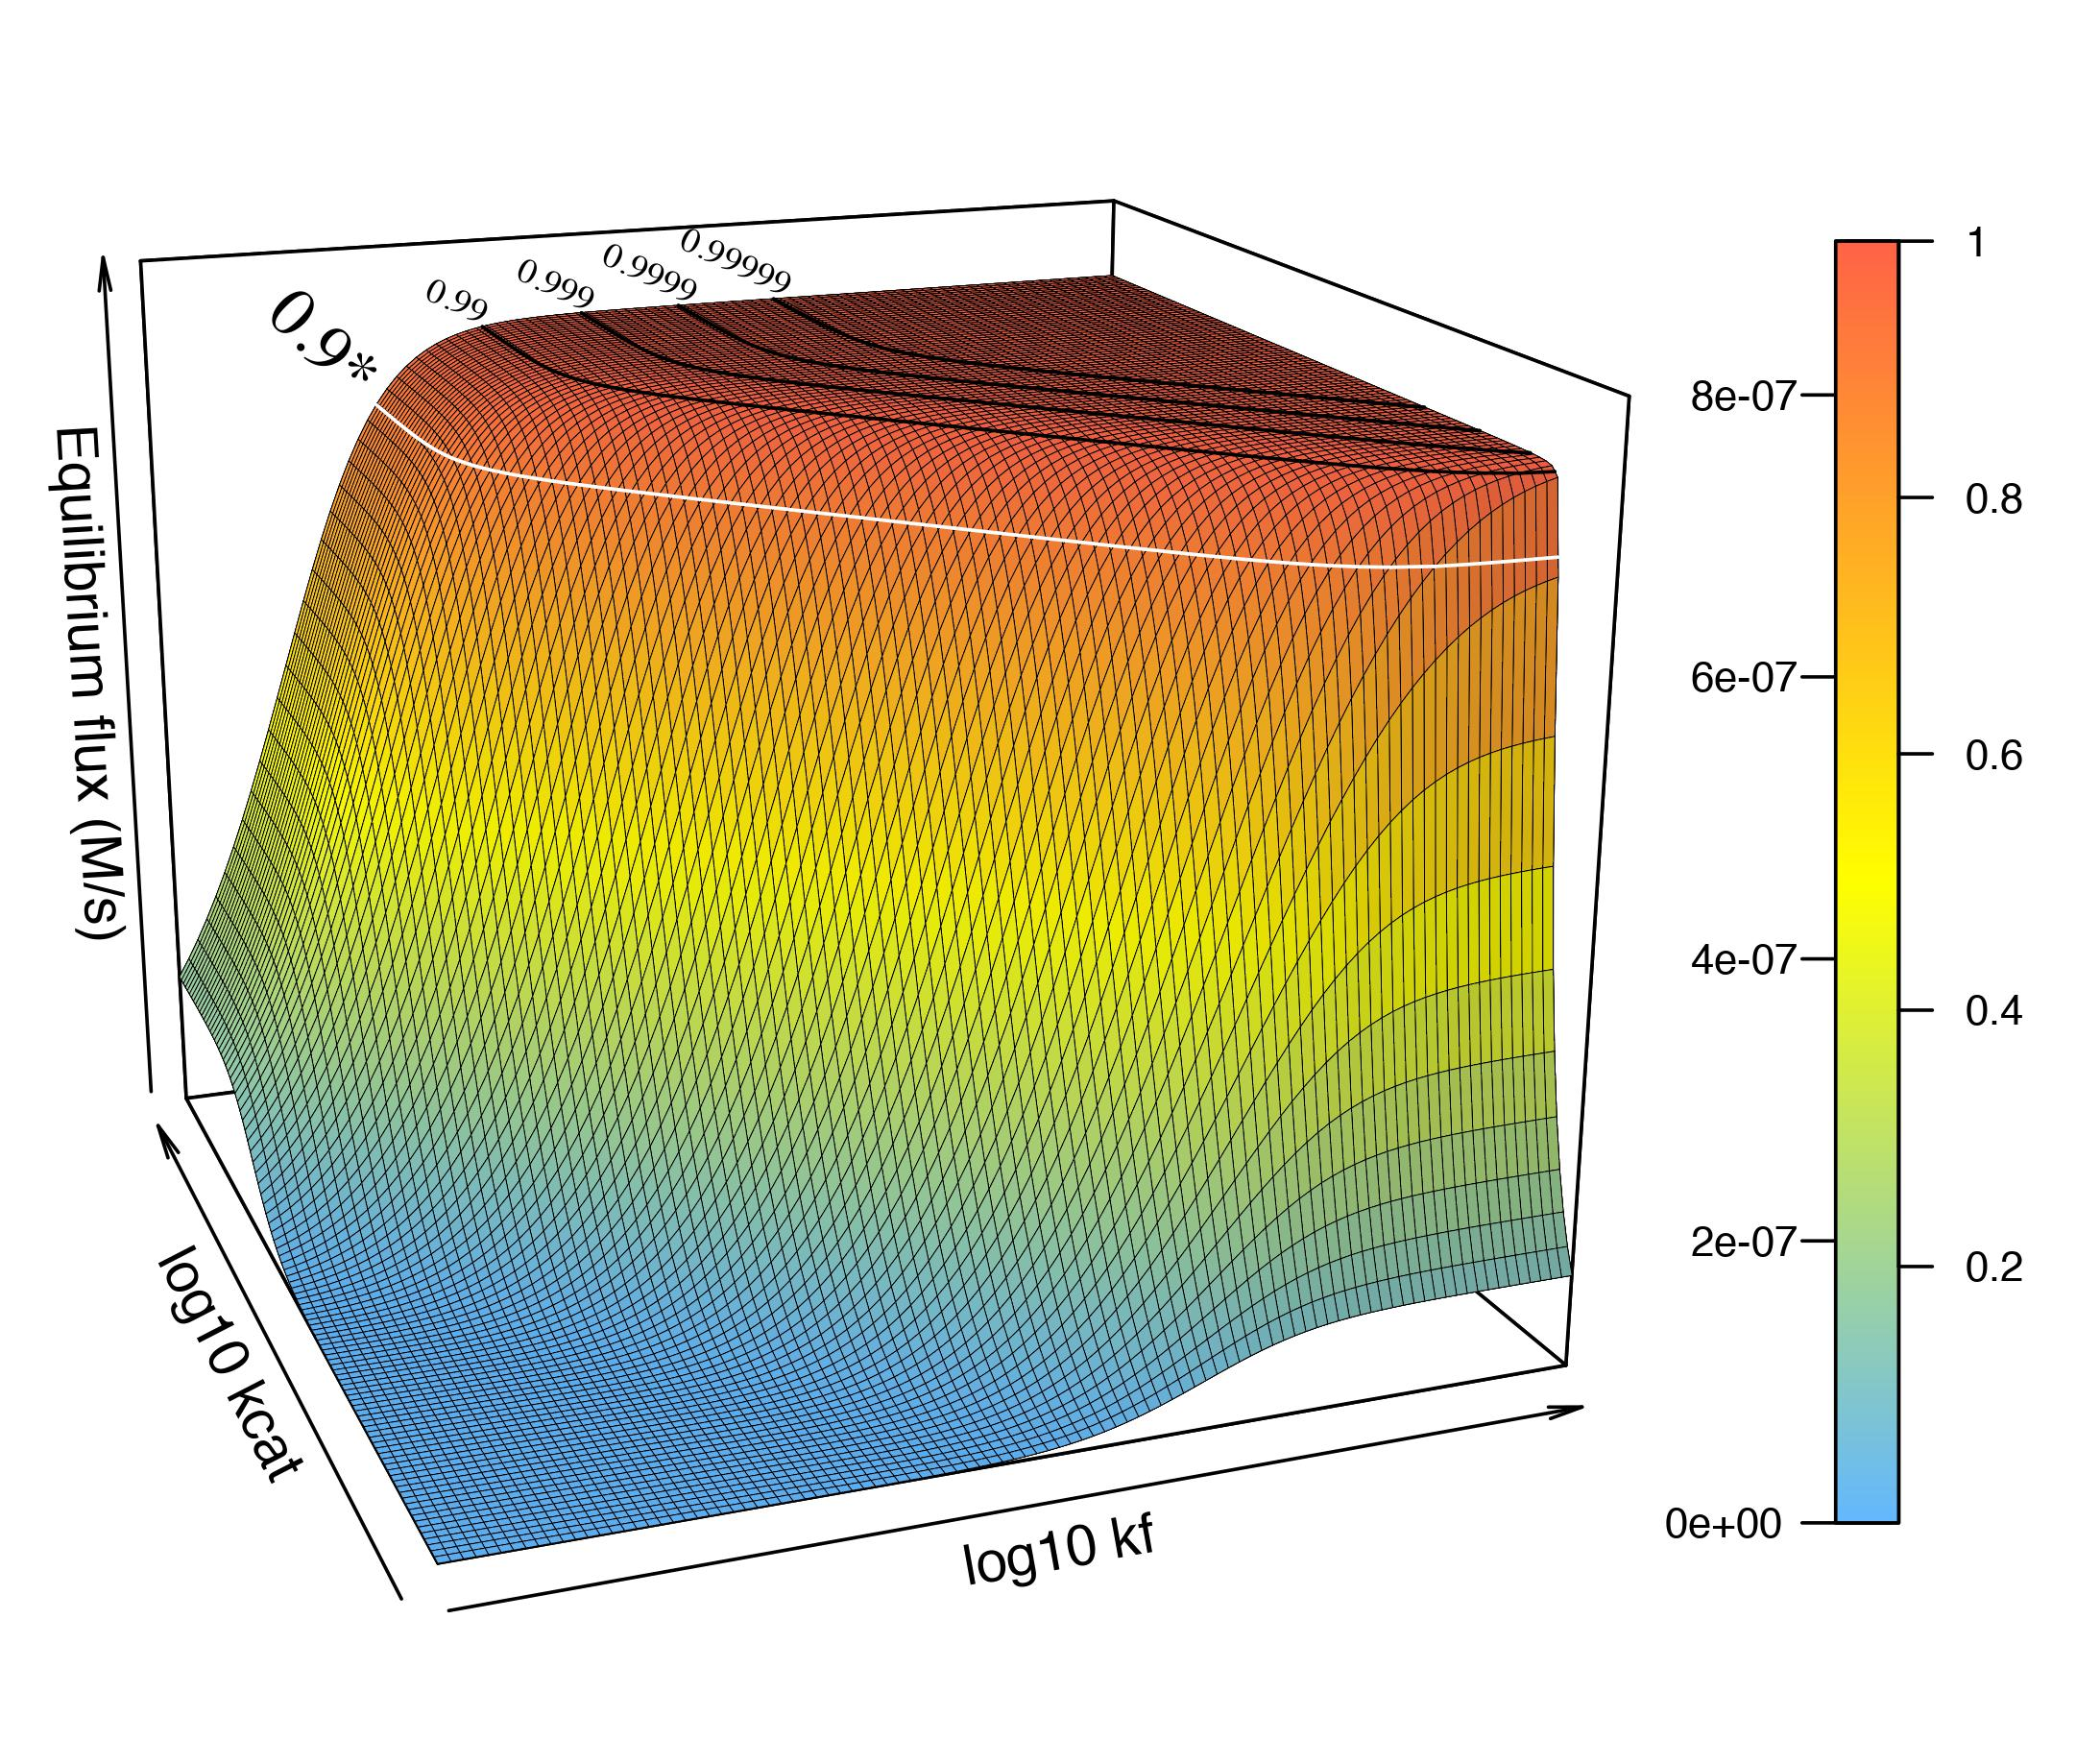
\includegraphics[scale=0.47,trim=0cm 0.75cm 0 1cm,clip]{Figures/3DFitLandscape.jpeg} 
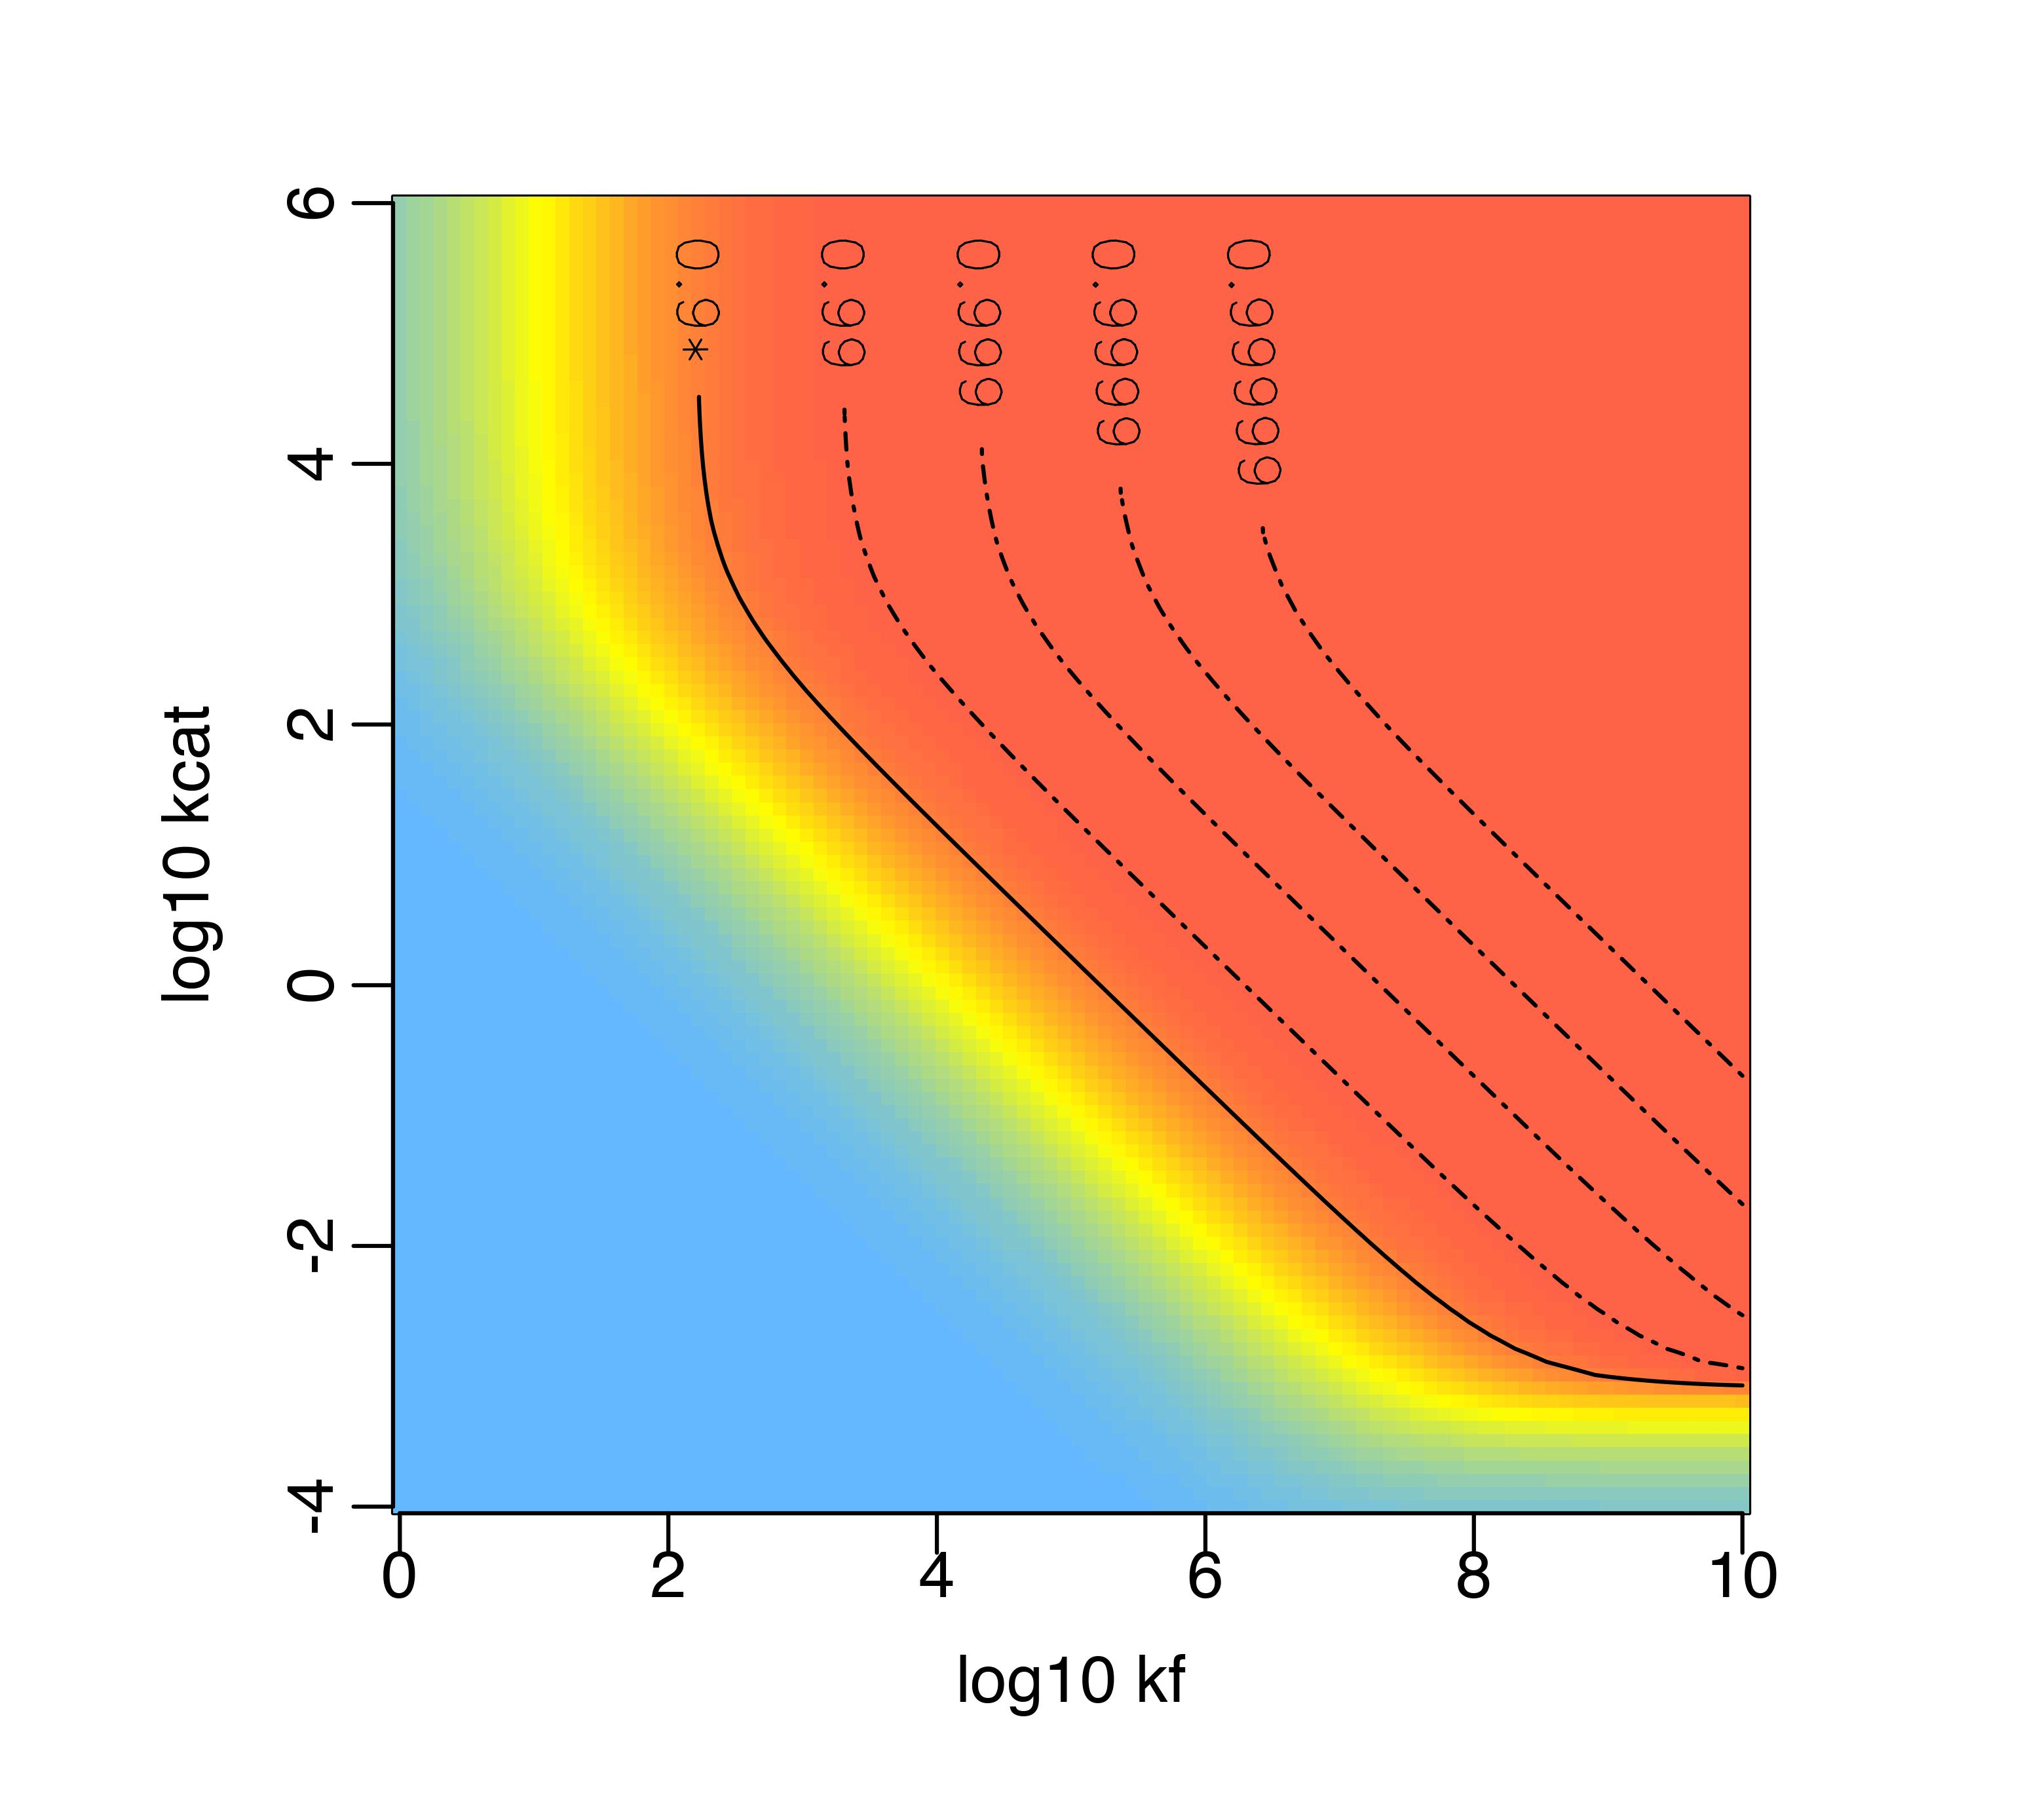
\includegraphics[scale=0.42,trim=0 0cm 0cm 1cm,clip]{Figures/2DFitLandscape.jpeg}  
\caption{The flux of product following substrate uptake by transporters and conversion by a dedicated enzyme depends on \DIFdelbeginFL \DIFdelFL{the }\DIFdelendFL kinetic parameters $k_f$ and $k_\text{cat}$\DIFdelbeginFL \DIFdelFL{of the enzyme}\DIFdelendFL . This landscape is \DIFdelbeginFL \DIFdelFL{generic in the sense that we avoid focusing }\DIFdelendFL \DIFaddbeginFL \DIFaddFL{based }\DIFaddendFL on \DIFdelbeginFL \DIFdelFL{sugars -- arguably extreme cases in terms of flux intensity -- for }\DIFdelendFL a \DIFdelbeginFL \DIFdelFL{general description, considering a moderate }\DIFdelendFL \DIFaddbeginFL \DIFaddFL{moderately low }\DIFaddendFL flux at saturation $V_{Tm}=1 \mu M.s^{-1}$ close to those measured for amino acids and nucleosides in E.\textit{coli} \citep{Zampieri2019}. We also set the transport saturation ratio $[S_\text{out}]/K_\text{T}$ to 10 such that the FD process approaches saturation, and \DIFaddbeginFL \DIFaddFL{relatively }\DIFaddendFL high transporter affinity $K_\text{T}=50\mu M$, also in line with estimates for nucleosides \citep{Griffith96,Xie04}\DIFdelbeginFL \DIFdelFL{(see Material and Methods)}\DIFdelendFL . Other parameter values include $k_r=10^3s^{-1}$ and $[E_{tot}]=1mM$. The color gradient \DIFdelbeginFL \DIFdelFL{shows }\DIFdelendFL \DIFaddbeginFL \DIFaddFL{indicates }\DIFaddendFL the absolute and normalized (\DIFdelbeginFL \DIFdelFL{such that the }\DIFdelendFL \DIFaddbeginFL \DIFaddFL{with a }\DIFaddendFL maximum flux \DIFdelbeginFL \DIFdelFL{equals }\DIFdelendFL \DIFaddbeginFL \DIFaddFL{of }\DIFaddendFL $1$) values of equilibrium flux.
}
\label{figure3D2DFit}
\end{figure*}

In order to depict a fitness landscape representative of an average enzyme, we first consider a situation where transporters \DIFdelbegin \DIFdel{saturate at an intermediate external concentration of the substrate with an intermediate affinity }\DIFdelend \DIFaddbegin \DIFadd{induce a moderately low rate $V_{Tm}$ and saturate with a relatively high affinity $K_T$ }\DIFaddend (FIG.~\ref{figure3D2DFit}\DIFaddbegin \DIFadd{, notice that affinity increases when $K_T$ decreases}\DIFaddend ). In this situation, the inward \DIFdelbegin \DIFdel{equilibrium flux }\DIFdelend \DIFaddbegin \DIFadd{flux at steady-state }\DIFaddend (which, as argued in the introduction, can be considered representative of fitness) forms a plateau when the upstream enzyme in the metabolic pathway has high $k_\text{cat}$ and $k_f$. This low equilibrium flux elasticity coincides with the saturation theory \DIFdelbegin \DIFdel{\citep{Wright34, Kacser73}}\DIFdelend \DIFaddbegin \DIFadd{\citep{Wright34, Kacser73,Hartl85,Dykhuizen87,Dean95,Yi19}}\DIFaddend , especially with its version incorporating facilitated diffusion \DIFdelbegin \DIFdel{\citep{Kuile94}}\DIFdelend \DIFaddbegin \DIFadd{\citep{Kuile94,Dean95}}\DIFaddend . The flux plateau is delineated by parallel isoclines (solid and interrupted lines in FIG.~\ref{figure3D2DFit}) oriented in the bottom-right direction of the landscape for intermediate values of $k_\text{cat}$ and $k_f$, such that decreasing $k_f$ by one order of magnitude can be compensated by a similar increase in $k_\text{cat}$. While this mutual dependency holds even for high $k_f$ values as long as $k_\text{cat}$ is not critically low (\textit{i.e.} when $k_\text{cat}>10^{-3}$), it stops when $k_\text{cat}\geq 10^3$, where increasing $k_\text{cat}$ no longer improves fitness. 
%DIF > %% On ne peut pas faire le commentaire suivant en s'appuyant sur la fig 1
%DIF > This negative relationship in a part of the isocline depends on the dissociation rate of enzyme-substrate complexes, $k_r$. As $k_r$ decreases away from $k_{cat}$, the isocline progressively loses this oblique part (Fig.~\ref{figure3D2DFit}), a trend that will be fully appreciated below. 
Besides, the influence of $k_\text{cat}$ and $k_f$ is not strictly equivalent, since the increase in flux is more gradual in response to $k_f$. 

Furthermore, and contrary to the textbook picture whereby most biological reactions are not limited by diffusion at all \citep{Bar-Even11,Sweetlove18}, increasing an enzyme's association rate $k_f$ – be it through its diffusivity or its binding rate – may still enhance the equilibrium flux when diffusion is substantially faster than catalysis.

\subsection{Properties of facilitated diffusion modulate the landscape}

To explore the effect of FD kinetics on the evolution of enzymes in the metabolic pathway, we studied the influence of  $K_T$ -- the affinity of the transporter for the substrate -- and $V_{Tm}$ -- the maximum transport rate -- still assuming that the substrate is close to saturation ($[S_\text{out}]/K_T=10$). We \DIFdelbegin \DIFdel{considered ranges of empirical estimates for sugars (high flux with low to moderate affinity in FIG.~\ref{figure2DSEns}, \citep{Stein86d,Maier02}), nucleosides \citep{Griffith96} and amino acids \citep{Stein86d,Zampieri2019} (weak to moderate flux with moderate to high affinity in FIG.~\ref{figure2DSEns}).   
}%DIFDELCMD < 

%DIFDELCMD < \begin{figure*}[h!]
%DIFDELCMD < \centering
%DIFDELCMD < \includegraphics[scale=0.35,trim=0cm 0 0 0,clip]{Figures/Fit_Landscape2D_Sensitivity.jpeg} 
%DIFDELCMD < %%%
%DIFDELCMD < \caption{%
{%DIFAUXCMD
\DIFdelFL{Both the affinity and rate of a transporter have an impact on the (normalized) flux landscape for upstream enzymes, the black isocline (corresponding to $0.9$) delineates the fitness plateau. Each plot represents the landscape obtained with a pair of values for transporters affinity $K_T$ and saturation $V_{Tm}$. Moving one step to the right means that $V_{Tm}$ increases by 1.5 orders of magnitude -- from $10^{-6}$ (low flux) to $10^{-3} M.s^{-1}$ (high) -- and one step up means that $K_T$ decreases by 2 orders of magnitude, starting at $10^{-1}M$ (low affinity). Increasing $K_T$ extends the plateau only towards the left part of the landscape, allowing enzymes with lower $k_f$ on the plateau, whereas decreasing $V_{Tm}$ extends the plateau in both directions. Other parameter values: $k_r=1000/s$, $[E_{tot}]=1mM$ and $[S_{env}]=10 \times K_T$.}}
%DIFAUXCMD
%DIFDELCMD < \label{figure2DSEns}
%DIFDELCMD < \end{figure*}
%DIFDELCMD < 

%DIFDELCMD < %%%
\DIFdel{We }\DIFdelend find that increasing the transport flux $V_{Tm}$ exerts a positive selection pressure on kinetic parameters for the upstream enzyme (\textit{i.e.} for increasing $k_\text{cat}$ and $k_f$). The plateau is shifted accordingly \DIFaddbegin \DIFadd{(see FIG.~\ref{figure2DSSatStud}-A)}\DIFaddend , towards the top-right corner of the landscape, at a distance that corresponds to the magnitude of the change in $V_{Tm}$. Increasing the affinity of the transporter (\textit{i.e.} decreasing $K_T$), however, selects for higher $k_{f}$ (the isoclines are displaced to the right and the fold change is similar to that of $K_T$) but has no \DIFaddbegin \DIFadd{other }\DIFaddend visible influence on $k_\text{cat}$ \DIFaddbegin \DIFadd{than increasing its codependency with $k_f$}\DIFaddend , a result that holds regardless of the flux at saturation $V_{Tm}$ \DIFdelbegin \DIFdel{. 
}\DIFdelend \DIFaddbegin \DIFadd{(notice that we only considered high $V_{Tm}$s, larger than in the average case, because these cases are more likely to be under directional selection). 
}

\DIFaddend This specific effect on the affinity of the upstream enzyme is likely due to a competition between the transporter -- which can transport the substrate in both directions -- and the enzyme, which harvests the substrate at a rate that depends on the dissociation constant $K_D=k_r/k_f$. It should be noted that nutrients under lower demands -- \textit{e.g.} amino acids -- are generally less concentrated in the environment, often coinciding with a higher affinity of their transporter. Therefore, the possible combinations of flux and affinity likely occupy a restricted space of possibilities where flux and affinity are negatively linked \DIFaddbegin \DIFadd{\citep{Gudelj10,Bosdriesz18}}\DIFaddend , which as can be seen in \DIFdelbegin \DIFdel{FIG.~\ref{figure2DSEns}-A}\DIFdelend \DIFaddbegin \DIFadd{SM Figs.~S3-A}\DIFaddend ,E,I results in landscapes that mainly differ by the minimum value of $k_\text{cat}$ on the plateau. \DIFaddbegin \DIFadd{In FIG.~\ref{figure2DSSatStud}-A, we have considered ranges of empirical estimates for sugars (high flux with low to moderate affinity) \citep{Stein86d,Maier02}, nucleosides \citep{Griffith96} and amino acids \citep{Stein86d,Zampieri2019} (weak to moderate flux with moderate to high affinity), which indeed mainly correspond to these combinations.   
}\DIFaddend 


\DIFdelbegin %DIFDELCMD < \begin{figure}[h!]
%DIFDELCMD < %%%
\DIFdelendFL \DIFaddbeginFL \begin{figure*}[h!]
\DIFaddendFL \centering
\DIFdelbeginFL %DIFDELCMD < 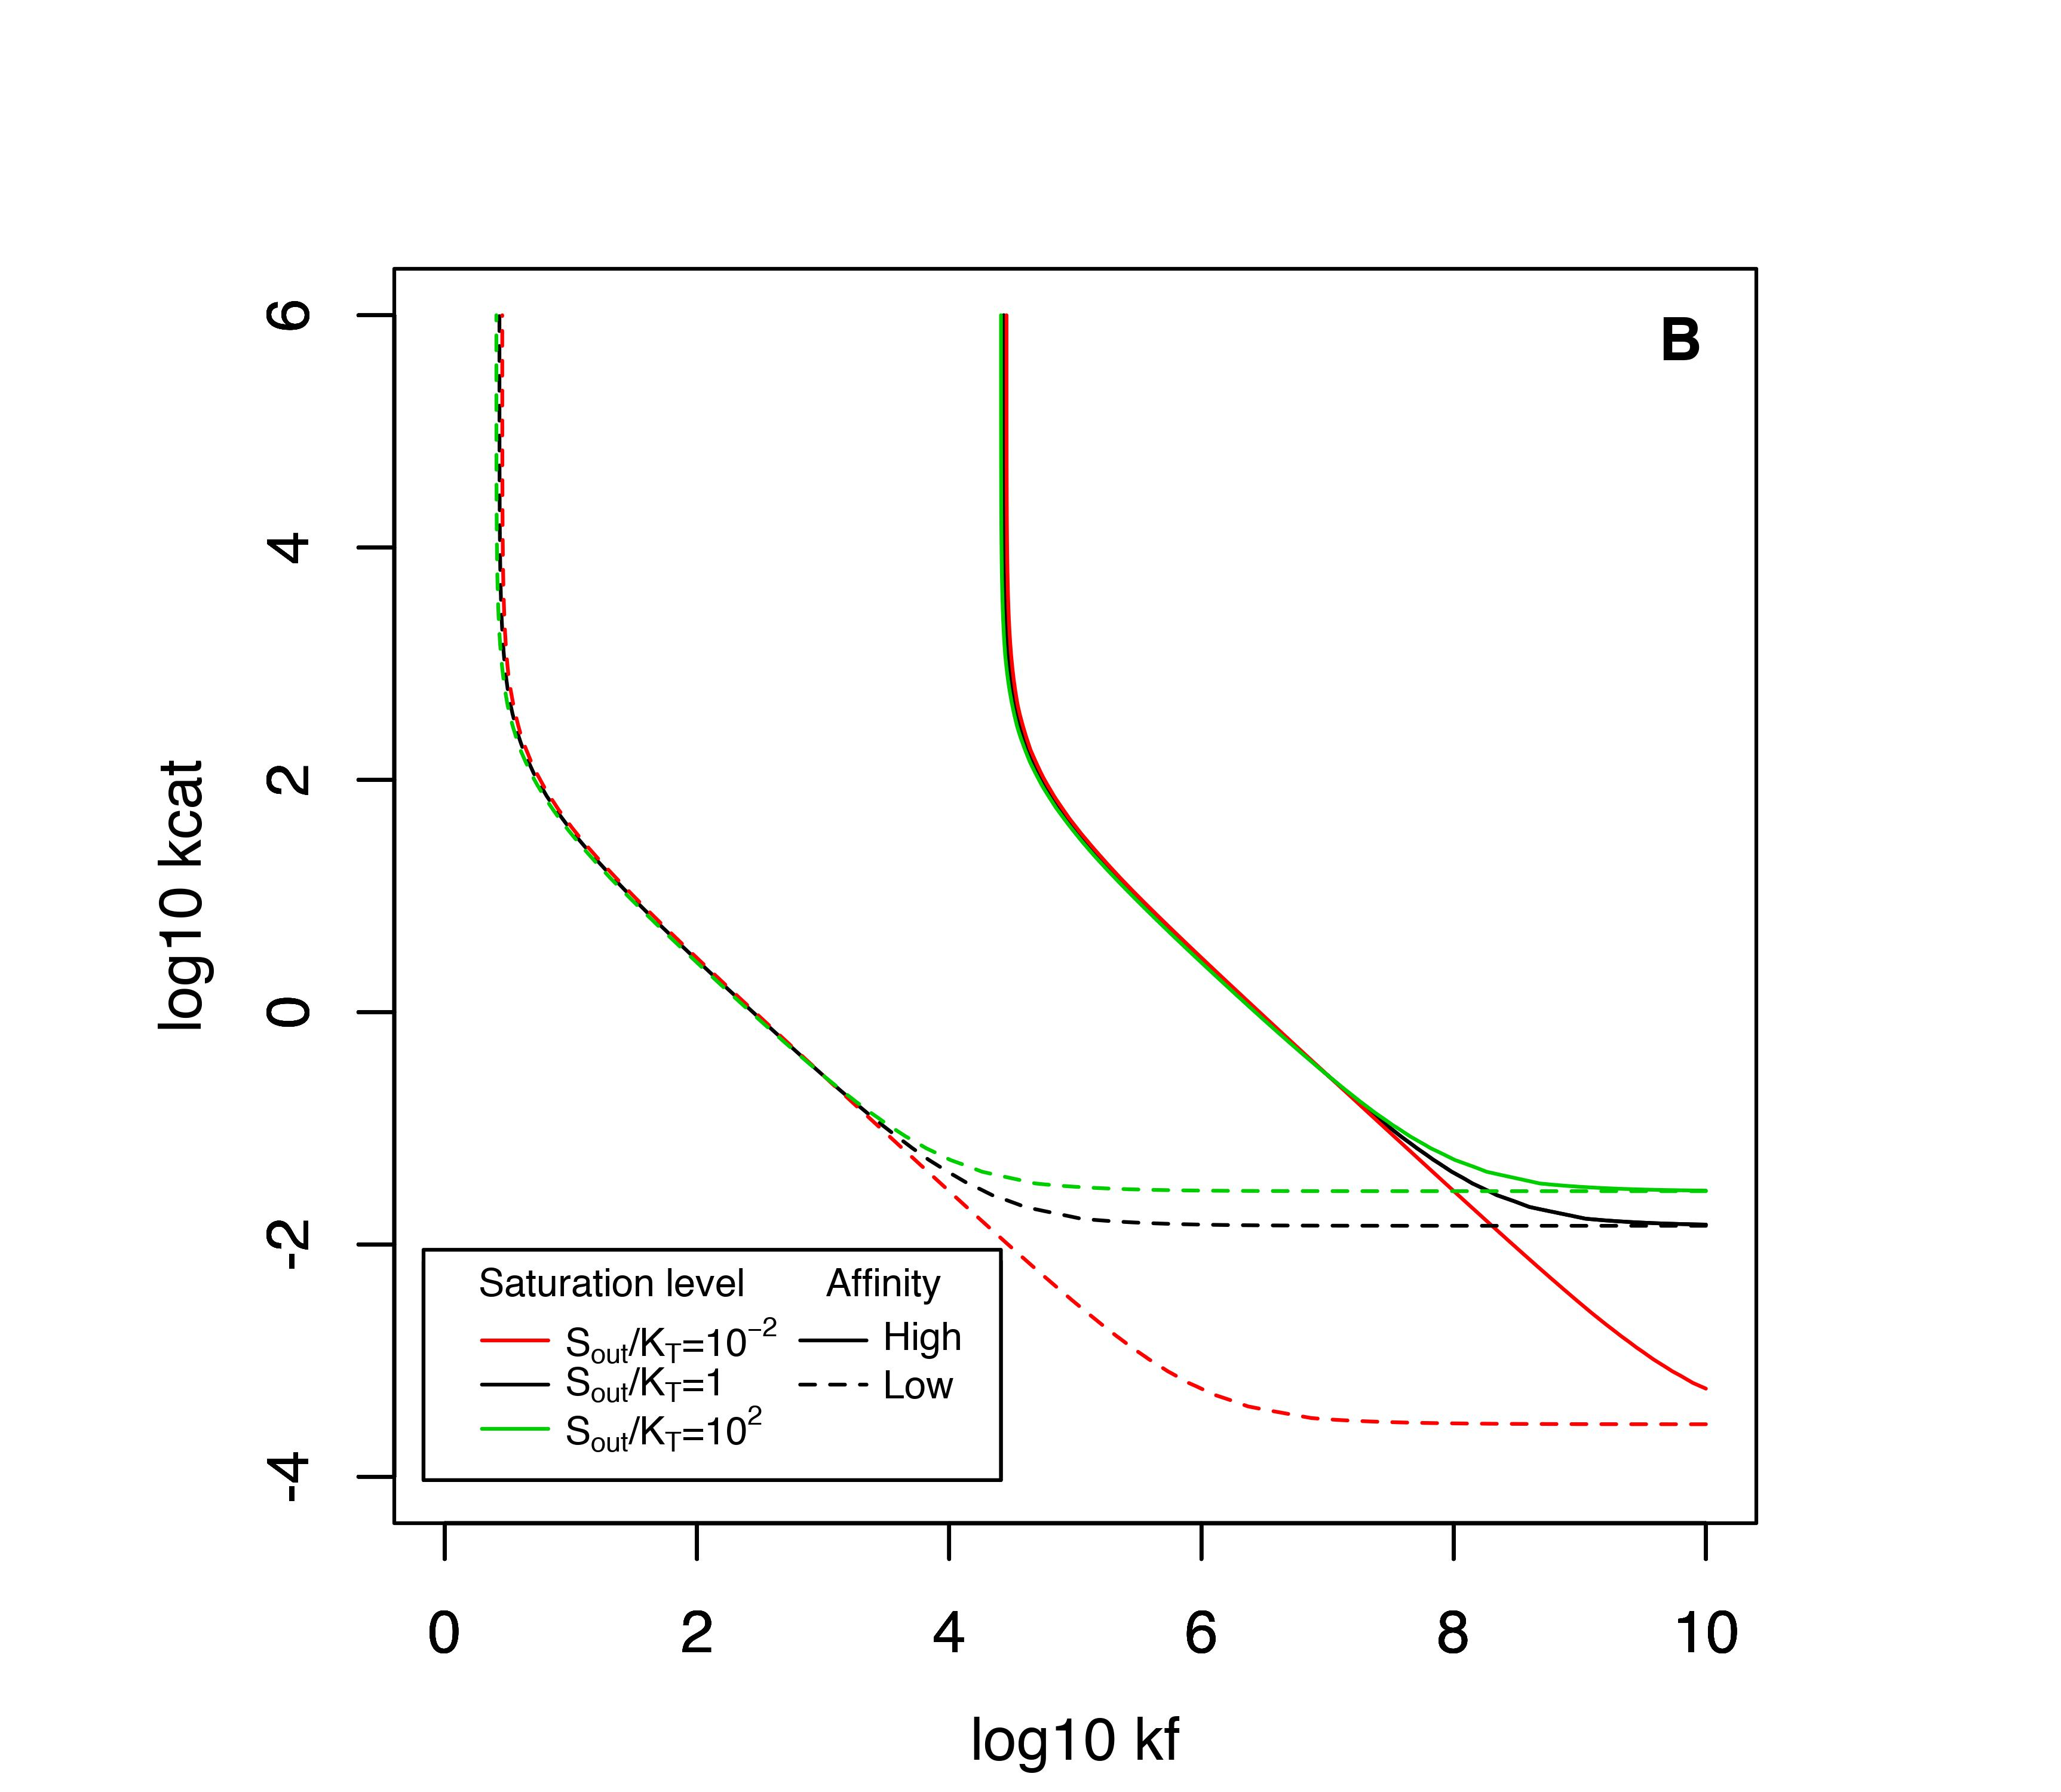
\includegraphics[scale=0.6,trim=0.5cm -0.3cm 0cm 1.5cm,clip]{Figures/2DFit_NonSatToSat.jpeg} 
%DIFDELCMD < %%%
\DIFdelendFL \DIFaddbeginFL 

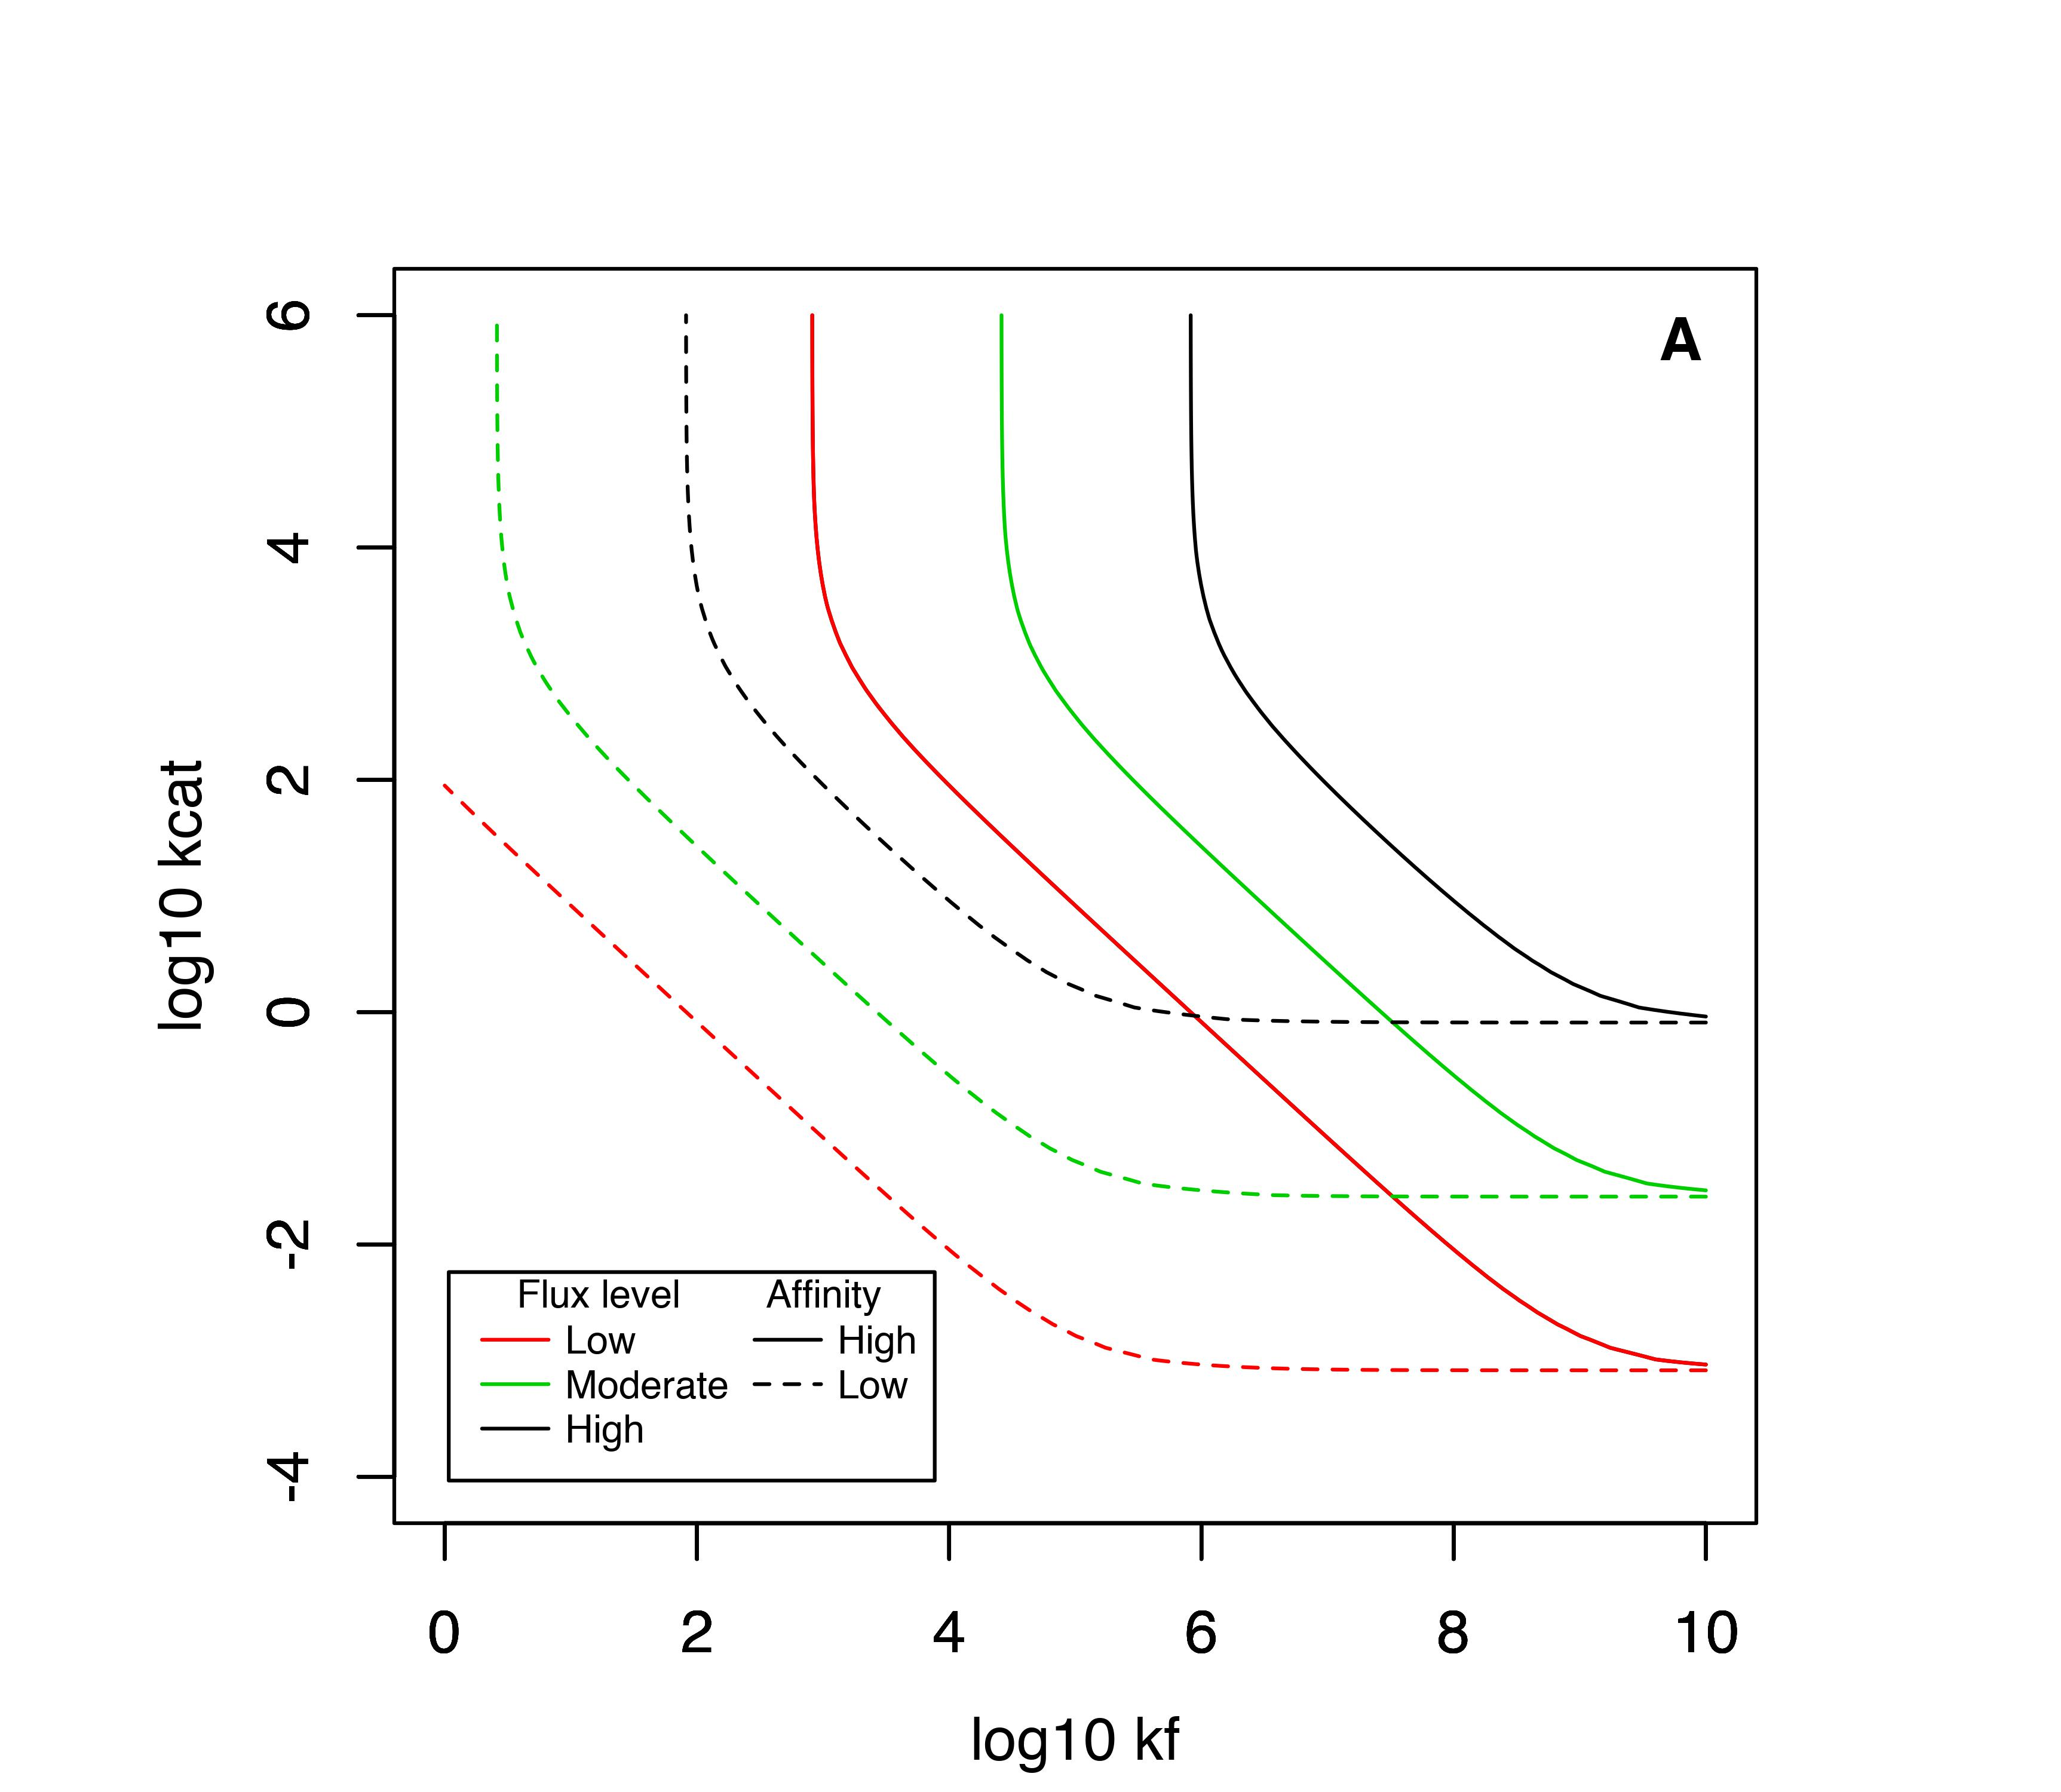
\includegraphics[scale=0.575,trim=0.5cm -0.3cm 0cm 1.5cm,clip]{Figures/2DFit_Flux_Sat.jpeg}
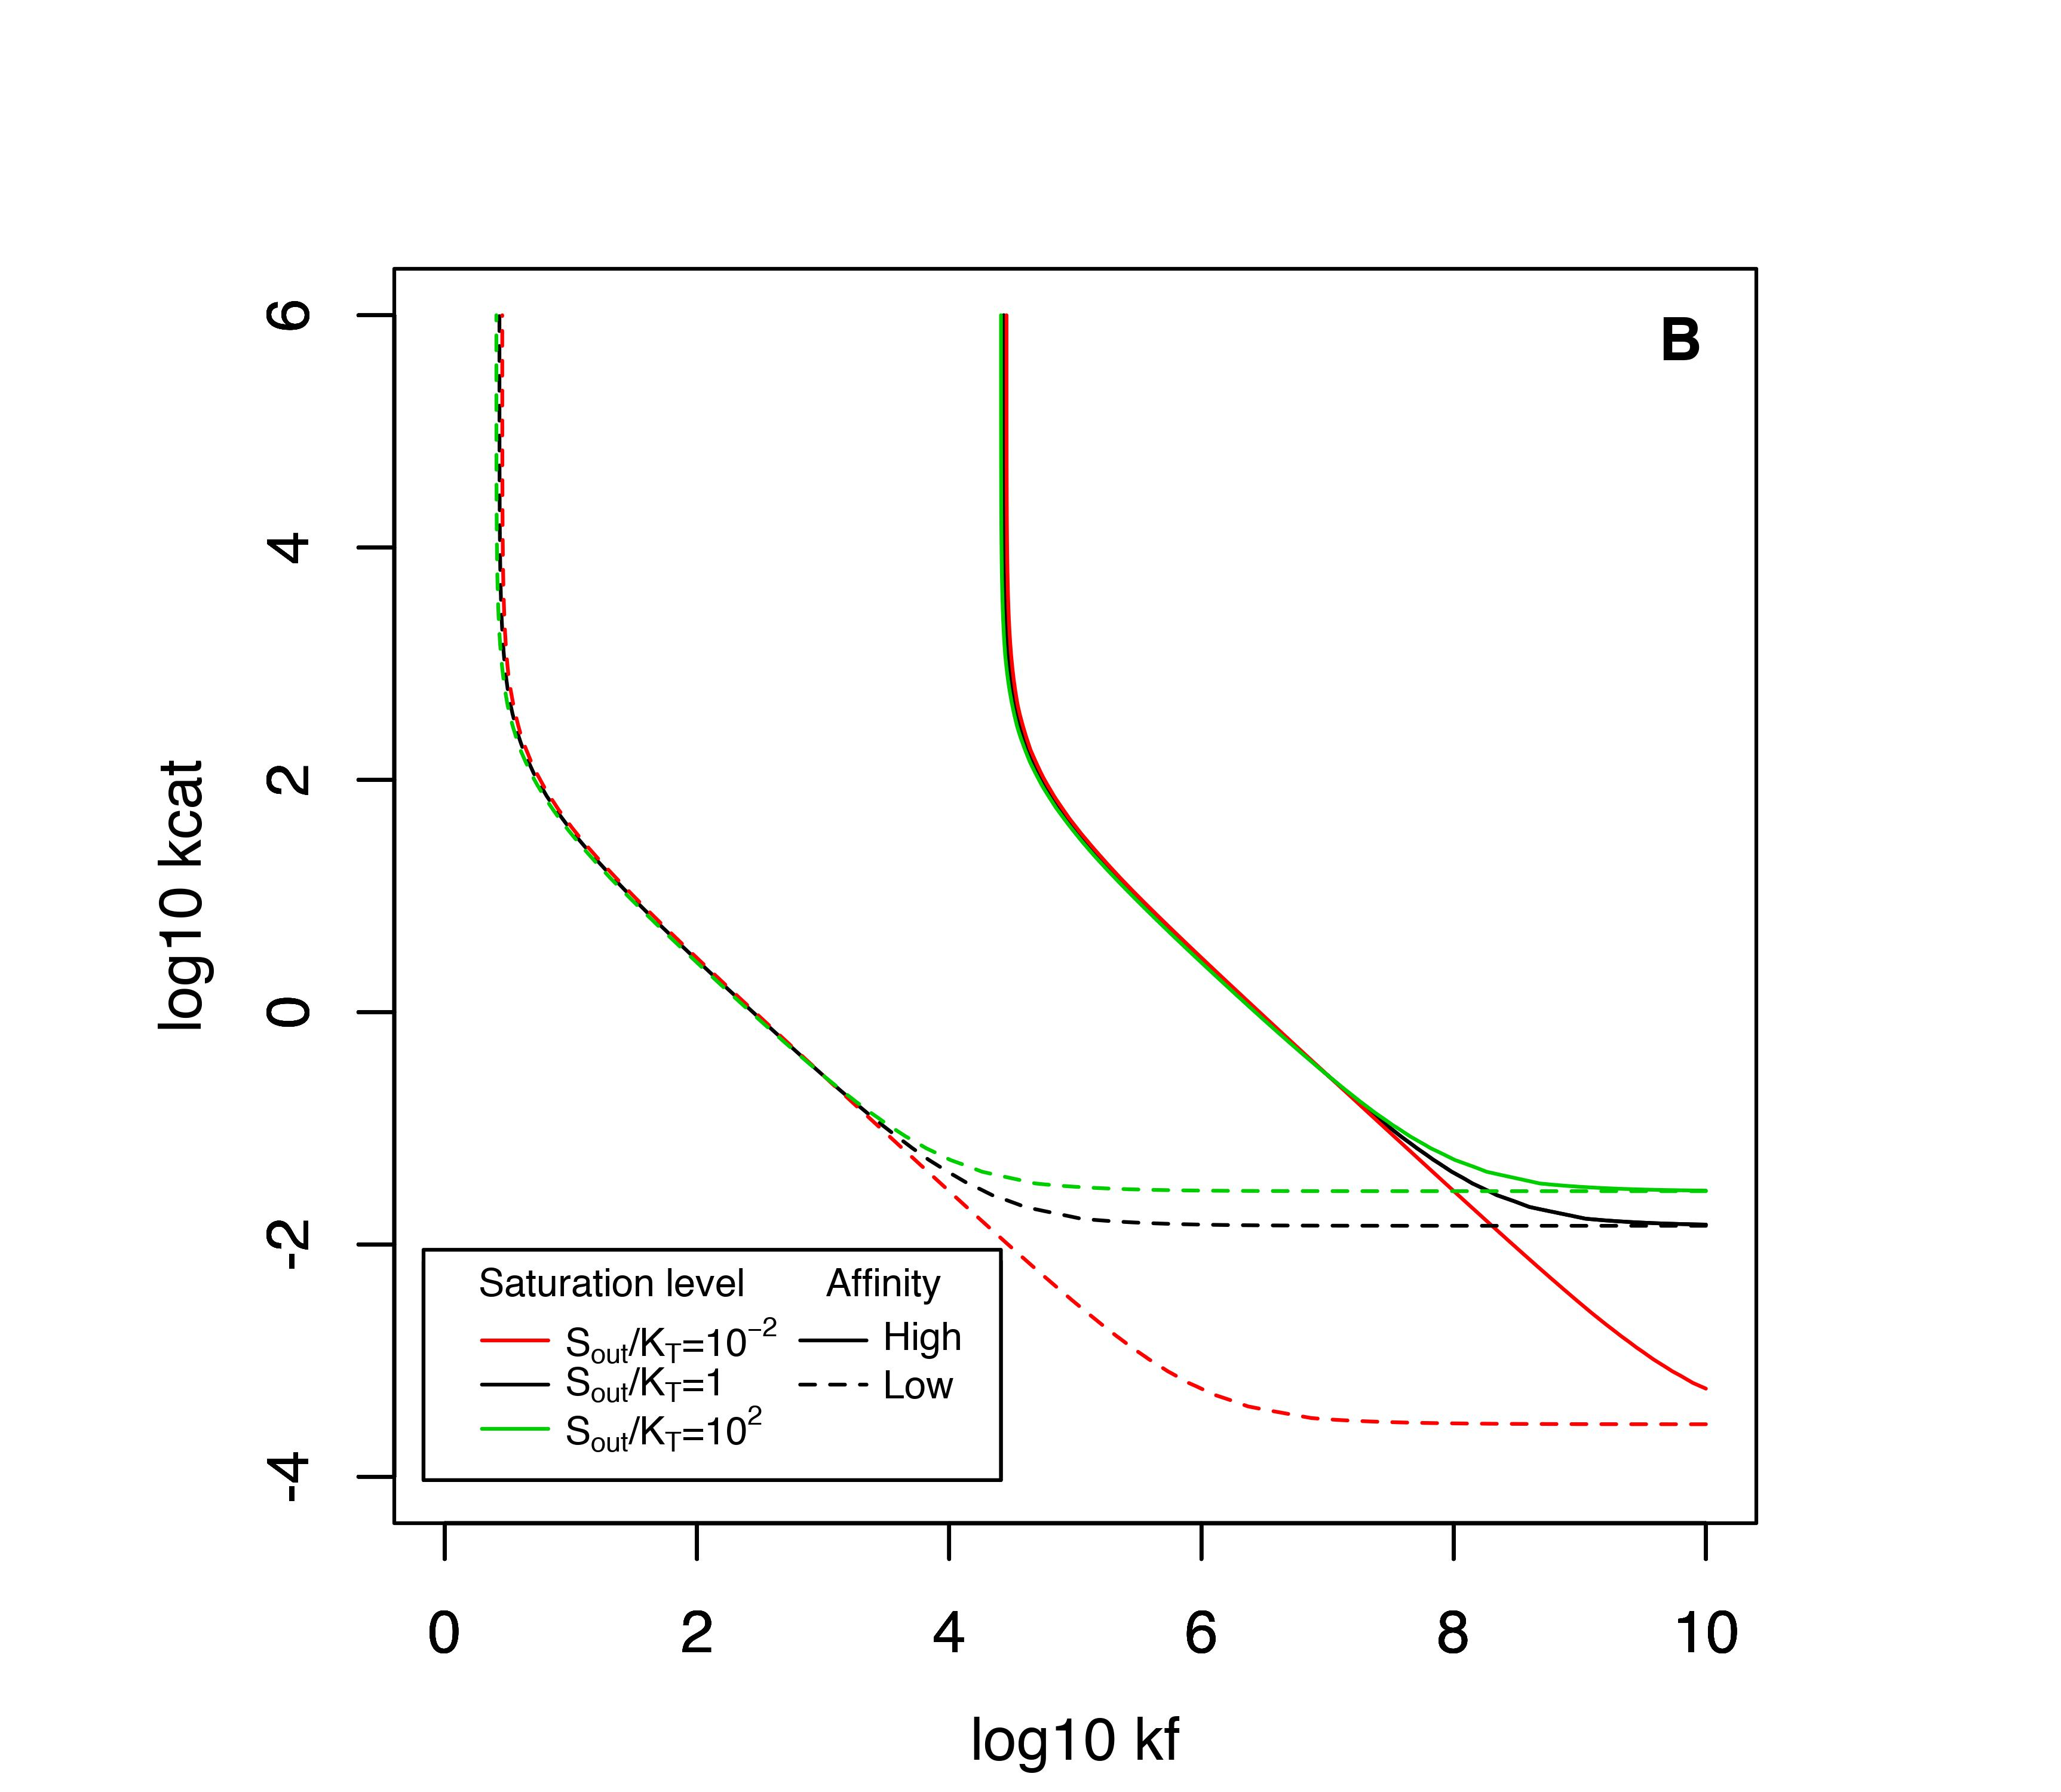
\includegraphics[scale=0.575,trim=0.5cm -0.3cm 0cm 1.5cm,clip]{Figures/2DFit_NonSatToSat.jpeg}
\DIFaddendFL \caption{\DIFdelbeginFL \DIFdelFL{The shape }\DIFdelendFL \DIFaddbeginFL \DIFaddFL{Features }\DIFaddendFL of \DIFaddbeginFL \DIFaddFL{a transporter have an impact on }\DIFaddendFL the \DIFdelbeginFL \DIFdelFL{fitness plateau -- represented }\DIFdelendFL \DIFaddbeginFL \DIFaddFL{flux landscape }\DIFaddendFL for \DIFdelbeginFL \DIFdelFL{each condition through }\DIFdelendFL \DIFaddbeginFL \DIFaddFL{upstream enzymes, as shown by }\DIFaddendFL the $0.9$ \DIFdelbeginFL \DIFdelFL{isocline (see FIG.~\ref{figure3D2DFit} for details) }\DIFdelendFL \DIFaddbeginFL \DIFaddFL{isoclines }\DIFaddendFL -- \DIFaddbeginFL \DIFaddFL{above which the relative flux }\DIFaddendFL is \DIFdelbeginFL \DIFdelFL{little dependent on }\DIFdelendFL \DIFaddbeginFL \DIFaddFL{$>90\%$ -- that delineate }\DIFaddendFL the \DIFdelbeginFL \DIFdelFL{saturation }\DIFdelendFL \DIFaddbeginFL \DIFaddFL{fitness plateau for each set }\DIFaddendFL of \DIFdelbeginFL \DIFdelFL{the }\DIFdelendFL \DIFaddbeginFL \DIFaddFL{parameter. A: low ($K_T=0.1M$) and high ($10\mu M$) }\DIFaddendFL transporter \DIFaddbeginFL \DIFaddFL{affinities are considered, in combination with low ($V_{Tm}=10^{-6} M$), moderate ($10^{-4.5} M$) or high maximum flux ($10^{-3} M$)}\DIFaddendFL . \DIFdelbeginFL \DIFdelFL{Only }\DIFdelendFL \DIFaddbeginFL \DIFaddFL{Increasing $K_T$ extends the plateau only towards the left part of the landscape, allowing }\DIFaddendFL enzymes \DIFdelbeginFL \DIFdelFL{downstream low affinity transporters show slightly relaxed selection }\DIFdelendFL \DIFaddbeginFL \DIFaddFL{with lower $k_f$ }\DIFaddendFL on \DIFdelbeginFL \DIFdelFL{$k_\text{cat}$ when }\DIFdelendFL the \DIFdelbeginFL \DIFdelFL{external concentration }\DIFdelendFL \DIFaddbeginFL \DIFaddFL{plateau, whereas decreasing $V_{Tm}$ extends the plateau in both directions. B: the shape }\DIFaddendFL of the \DIFdelbeginFL \DIFdelFL{substrate }\DIFdelendFL \DIFaddbeginFL \DIFaddFL{fitness plateau }\DIFaddendFL is \DIFdelbeginFL \DIFdelFL{lower than }\DIFdelendFL \DIFaddbeginFL \DIFaddFL{however little dependent on }\DIFaddendFL the \DIFdelbeginFL \DIFdelFL{affinity constant }\DIFdelendFL \DIFaddbeginFL \DIFaddFL{saturation }\DIFaddendFL of the transporter, \DIFdelbeginFL \DIFdelFL{$K_T$. The example shown is }\DIFdelendFL for a transporter with moderate flux ($V_{Tm}=10^{-4.5}M.s^{-1}$\DIFdelbeginFL \DIFdelFL{)}\DIFdelendFL ; the effect is identical for \DIFdelbeginFL \DIFdelFL{other }\DIFdelendFL \DIFaddbeginFL \DIFaddFL{higher }\DIFaddendFL $V_{Tm}$\DIFdelbeginFL \DIFdelFL{(}\DIFdelendFL \DIFaddbeginFL \DIFaddFL{, }\DIFaddendFL see \DIFdelbeginFL \DIFdelFL{Figure S2 of }\DIFdelendFL SM \DIFaddbeginFL \DIFaddFL{Fig. S2}\DIFaddendFL ). \DIFaddbeginFL \DIFaddFL{Other parameter values: $k_r=1000/s$, $[E_{tot}]=1mM$ and $[S_{env}]=10 \times K_T$.}\DIFaddendFL }
\label{figure2DSSatStud}
\DIFdelbeginFL %DIFDELCMD < \end{figure}
%DIFDELCMD < %%%
\DIFdelend \DIFaddbegin \end{figure*}
\DIFaddend 

So far we have considered transporters saturated by high external substrate concentrations. Relaxing this assumption has little impact on the fitness landscape, except that very low values of $k_\text{cat}$ (\DIFdelbegin \DIFdel{\textit{i.e.} }\DIFdelend lower than $10^{-2}$ \DIFaddbegin \DIFadd{in FIG. \ref{figure2DSSatStud}-B}\DIFaddend ) can only sustain \DIFdelbegin \DIFdel{high fluxes at saturation(see }\DIFdelend \DIFaddbegin \DIFadd{the low influx of transporters far from saturation, but fail to keep up with higher influxes in richer environments. 
}

\subsection{\DIFadd{Enzymes differ among metabolic pathways}}

\begin{figure}[h!]
\centering
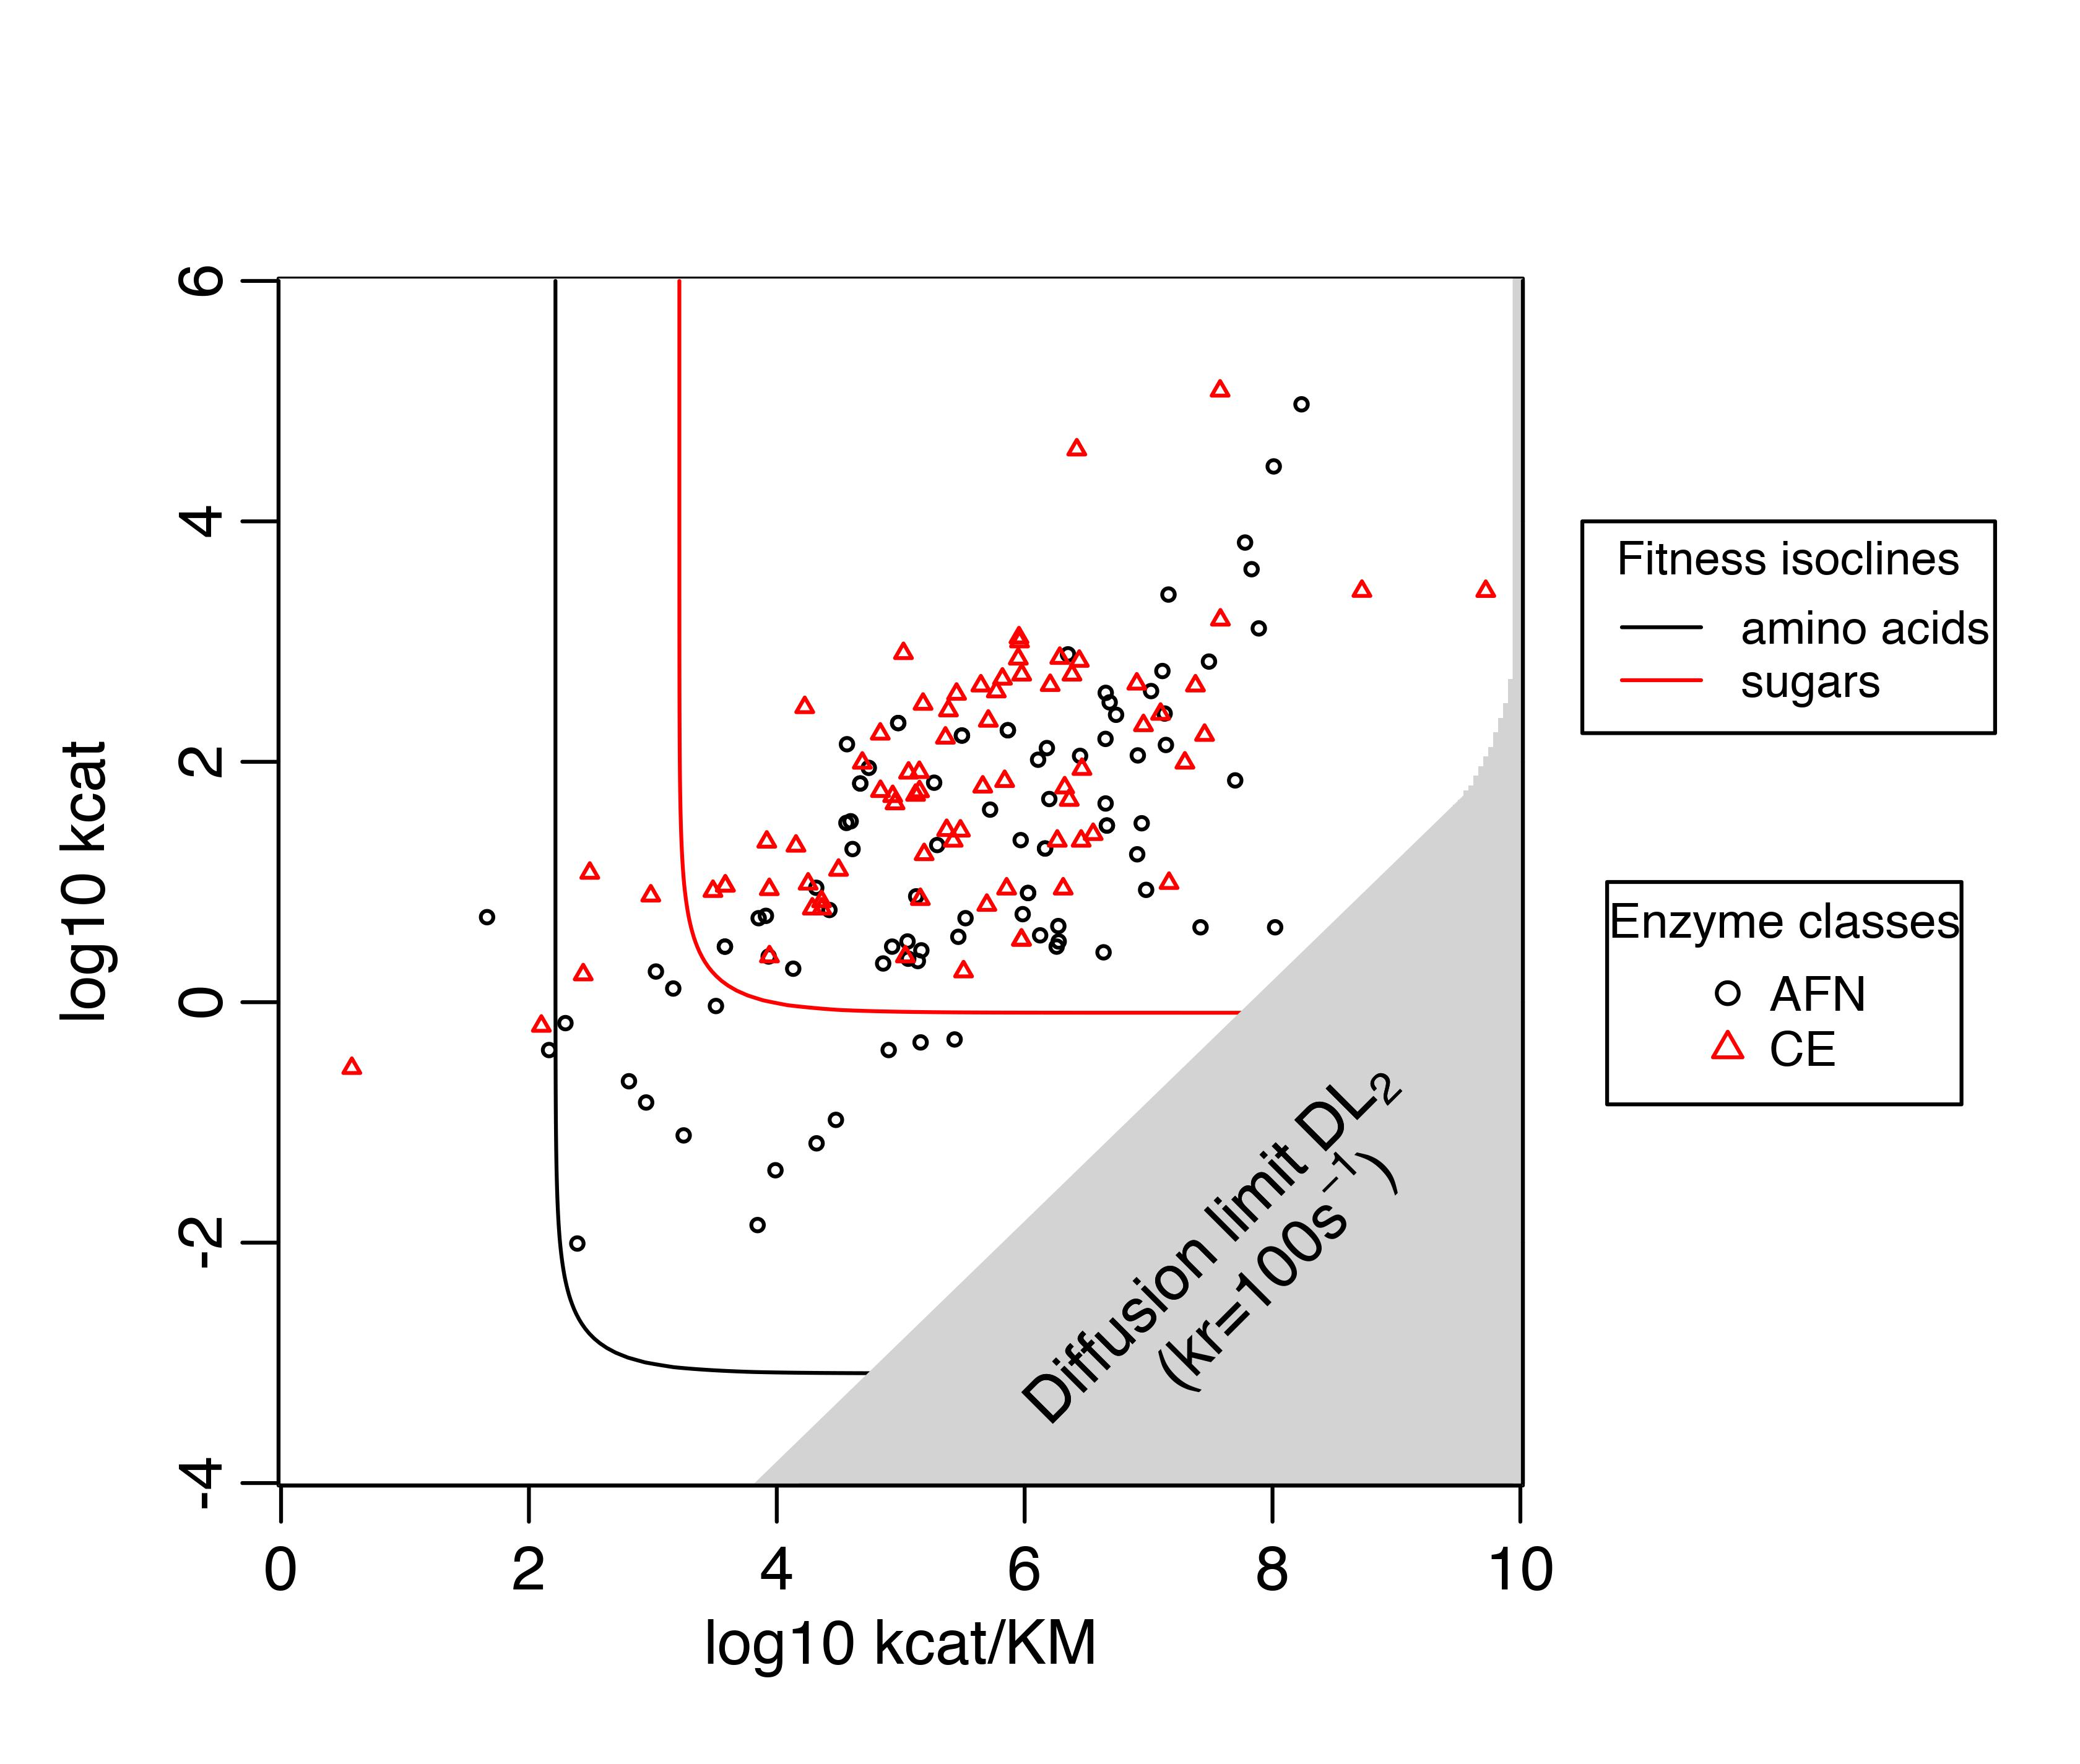
\includegraphics[scale=0.55,trim=0cm 0cm 0cm 1.5cm,clip]{Figures/2DFitContour_DataClasses.jpeg}  
\othercaption{\textit{in vitro} experimental estimates of kinetic parameters $k_\text{cat}$ and $k_\text{cat}/K_\text{M}$ exhibit different distributions for enzymes involved in different categories of pathways -- as identified by \citet{Bar-Even11} -- namely (AFN): amino acids, fatty acids, and nucleotides and (CE): carbohydrates and energy. Corresponding fitness landscapes -- differing by transporter features -- are superimposed, with the parameter space narrowed down due to the diffusion limit (grey area, set for $k_r=10^2 s^{-1}$). The isoclines shown correspond to parameter values typical of sugar transporters ($K_T=5mM$,$V_{Tm}=1mM.s^{-1}$, in red) \citep{Maier02} or amino acids transporters (same as in FIG.~\ref{figure3D2DFit}, in black).}
\label{figure2D_BarEven_Dataset}
\end{figure}

\DIFadd{We then superimposed empirical estimates of kinetic parameters over our theoretical fitness landscapes, after substituting parameter $k_f$ for its usual empirical counterpart, $k_\text{cat} / K_\text{M}$. Because $k_{cat}/K_\text{M} = k_fk_{cat}/(k_r+k_{cat})$, this approximation only holds when $k_\text{cat} \gg k_r$. Representing the fitness landscape in this parameter space
sets an inaccessible area in the bottomright part of the landscapes where $k_f$ would exceed the diffusion limit (grey area on }\DIFaddend FIG.~\DIFdelbegin \DIFdel{\ref{figure2DSSatStud}). Diminishing returns shall thus be the rule for the first enzyme whatever the extracellular environment, }\DIFdelend \DIFaddbegin \DIFadd{\ref{figure2D_BarEven_Dataset}). For purposes of inclusiveness, we used $k_r=10^{2}s^{-1}$ by default -- noting that this limit would be displaced upwards for larger $k_r$ (and downwards otherwise).
}

\DIFadd{We otherwise used sets of parameters that correspond to typical features of sugar and amino acid/nucleoside transporters to obtain FIG.~\ref{figure2D_BarEven_Dataset}. Because we have previously shown that changing the affinity or maximum flux of transporters may move the fitness plateau, our model predicts that enzymes involved in the corresponding pathways (\textit{e.g.} of sugars and amino acids) should have their own specific distributions. We see that enzymes involved in the central carbohydrate metabolism as categorized by \citet{Bar-Even11} have on average higher $k_\text{cat}$ }\DIFaddend and \DIFdelbegin \DIFdel{this phenomenon typically occurs within the known behavioral range for both catalysts and transporters}\DIFdelend \DIFaddbegin \DIFadd{$K_\text{M}$ than those metabolising amino-acids and nucleotides. Our superimposition with the predicted fitness plateaus in FIG.~\ref{figure2D_BarEven_Dataset} suggests that there may indeed be an explainable difference between enzymes contributing to carbohydrate processing (in red) and to that of other primary metabolites (in black, \textit{e.g.} amino acids).
We acknowledge that this result implicitly suggests that enzymes within a pathway have evolved on a common fitness landscape, spreading neutrally onto the fitness plateau. This is by no means our interpretation, as this subset of the full dataset includes enzymes that differ in many other ways that, as we will see, make each enzyme evolve on its own fitness landscape and thereby potentially explain a large part of this observed variance}\DIFaddend . 

\subsection{Downstream enzymes also evolve on cliff-like fitness landscapes}

\begin{figure*}[t!]
\centering
\begin{minipage}[c]{0.48\linewidth}
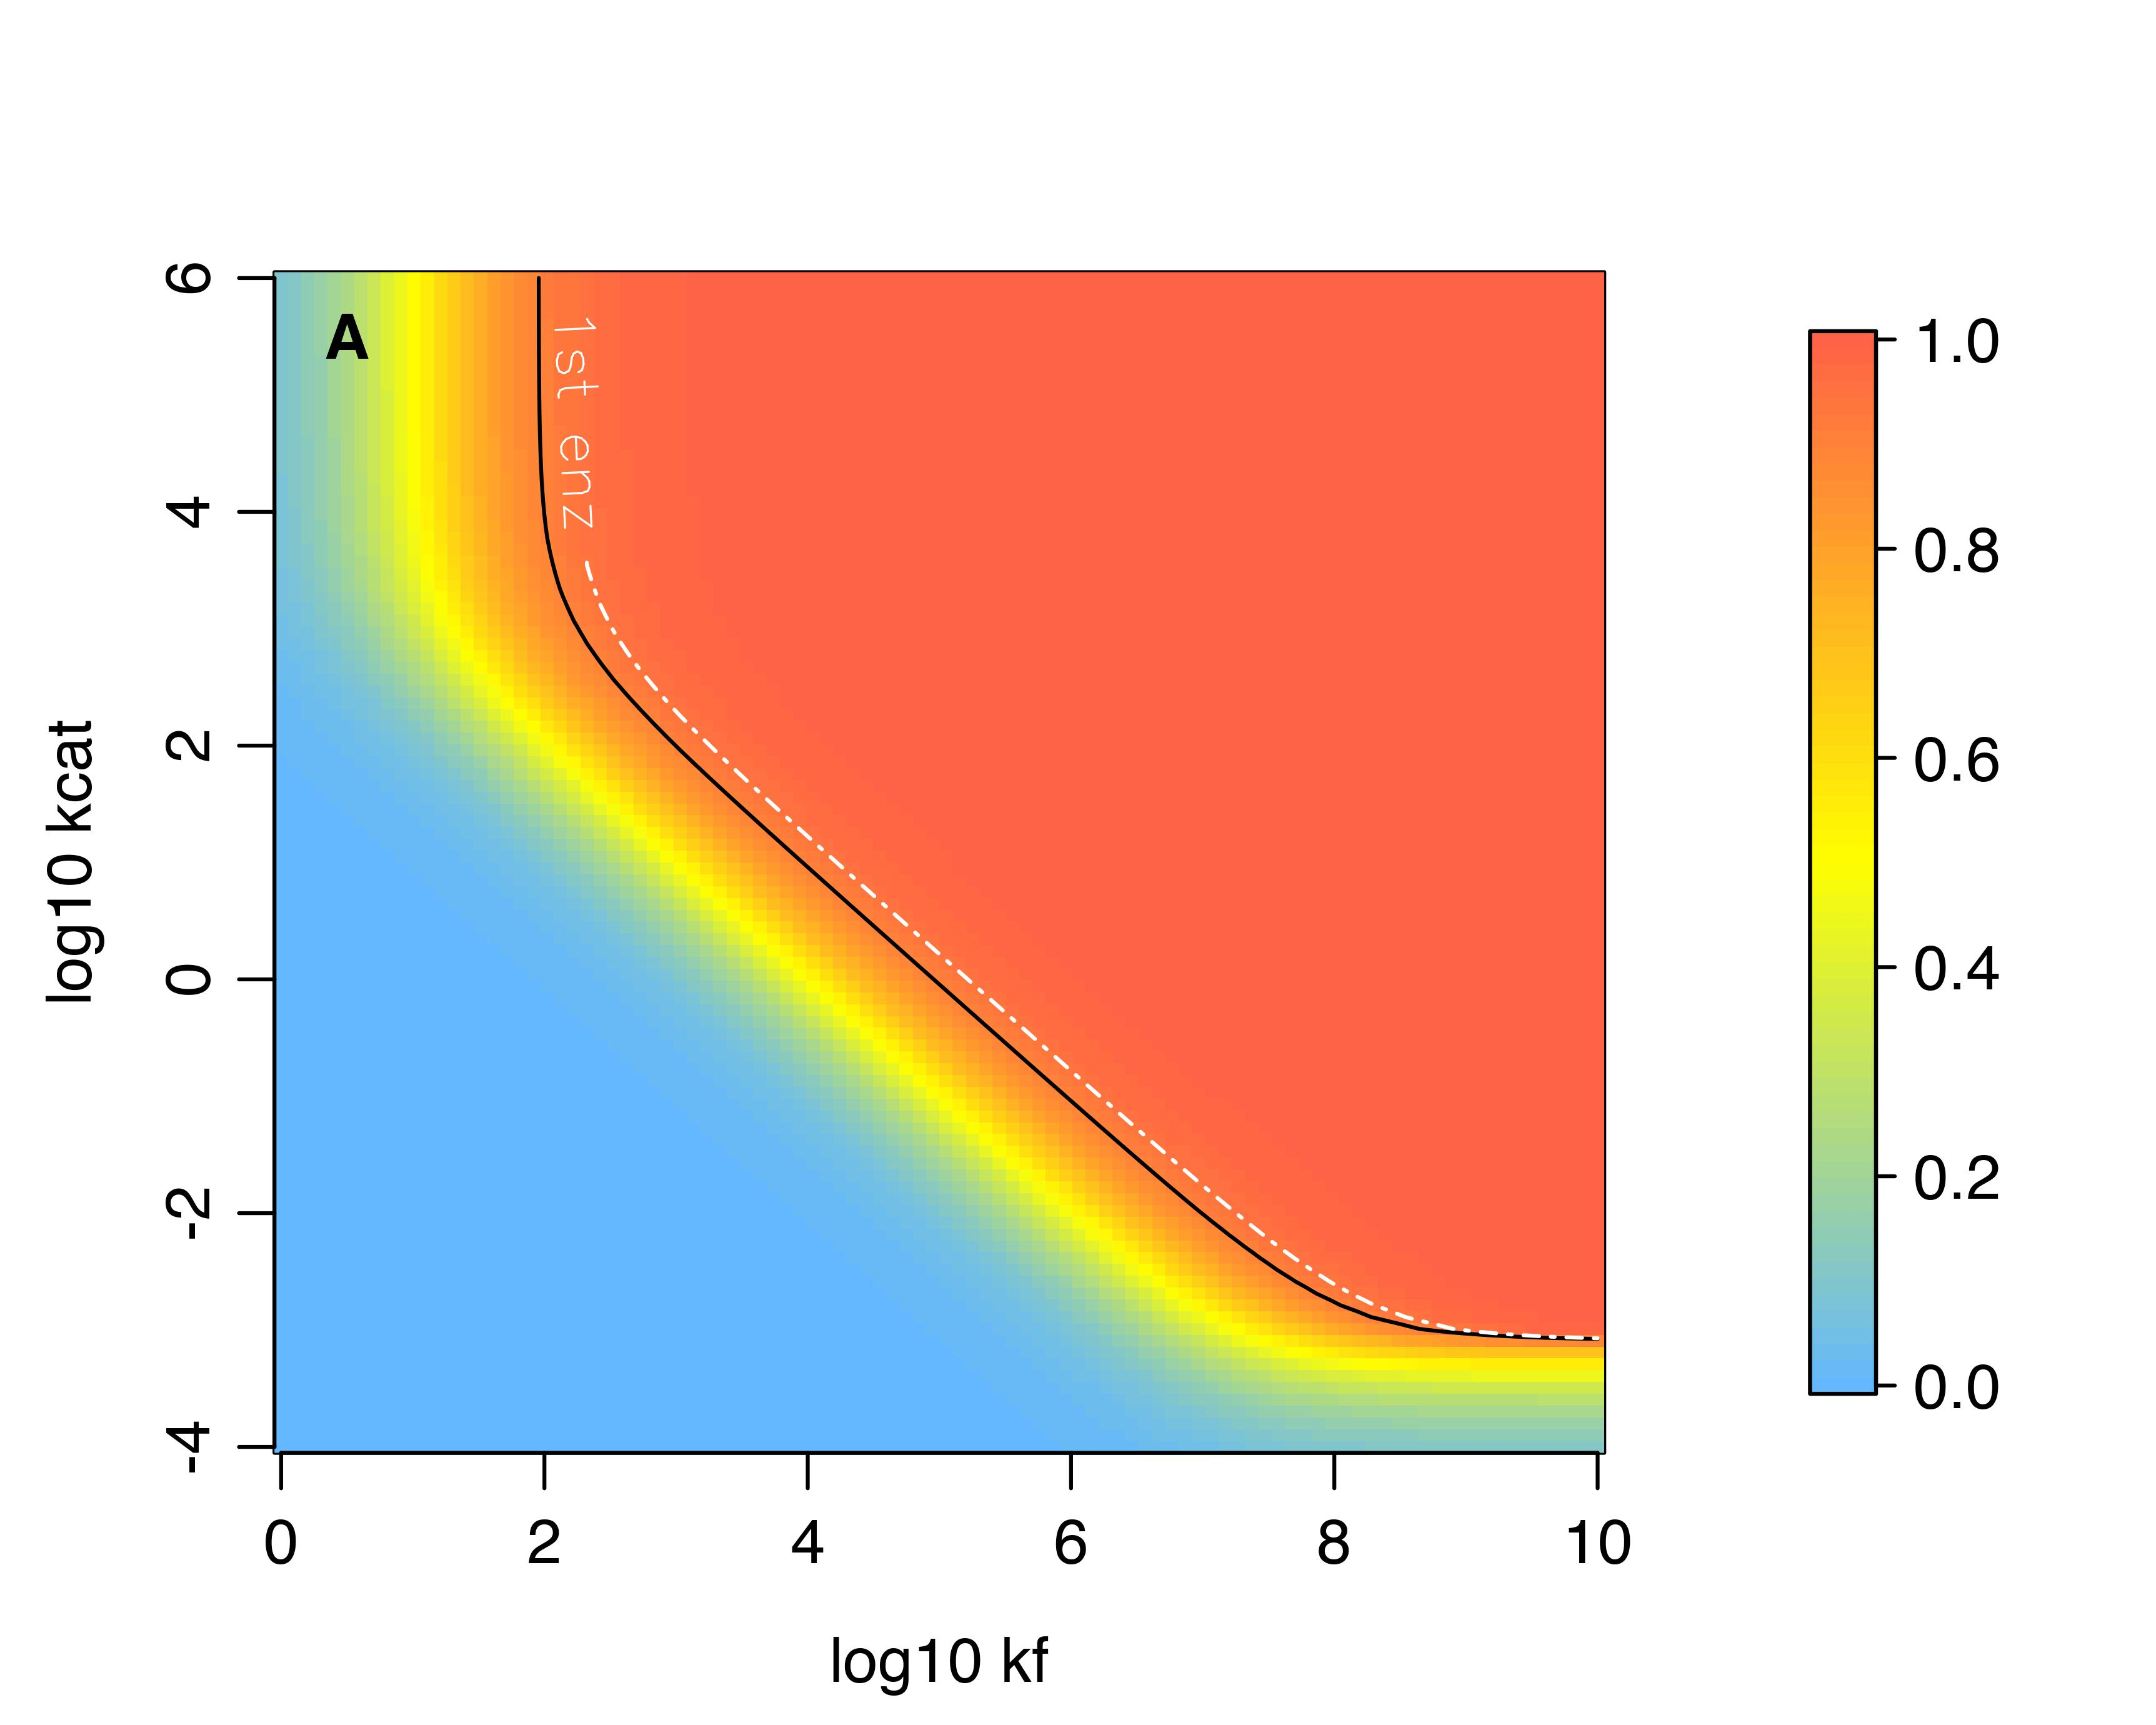
\includegraphics[scale=0.65,trim=0cm 0cm 0cm 1.5cm,clip]{Figures/2DFitLandscape_etahigh_noreverse.jpeg} 
%DIF > 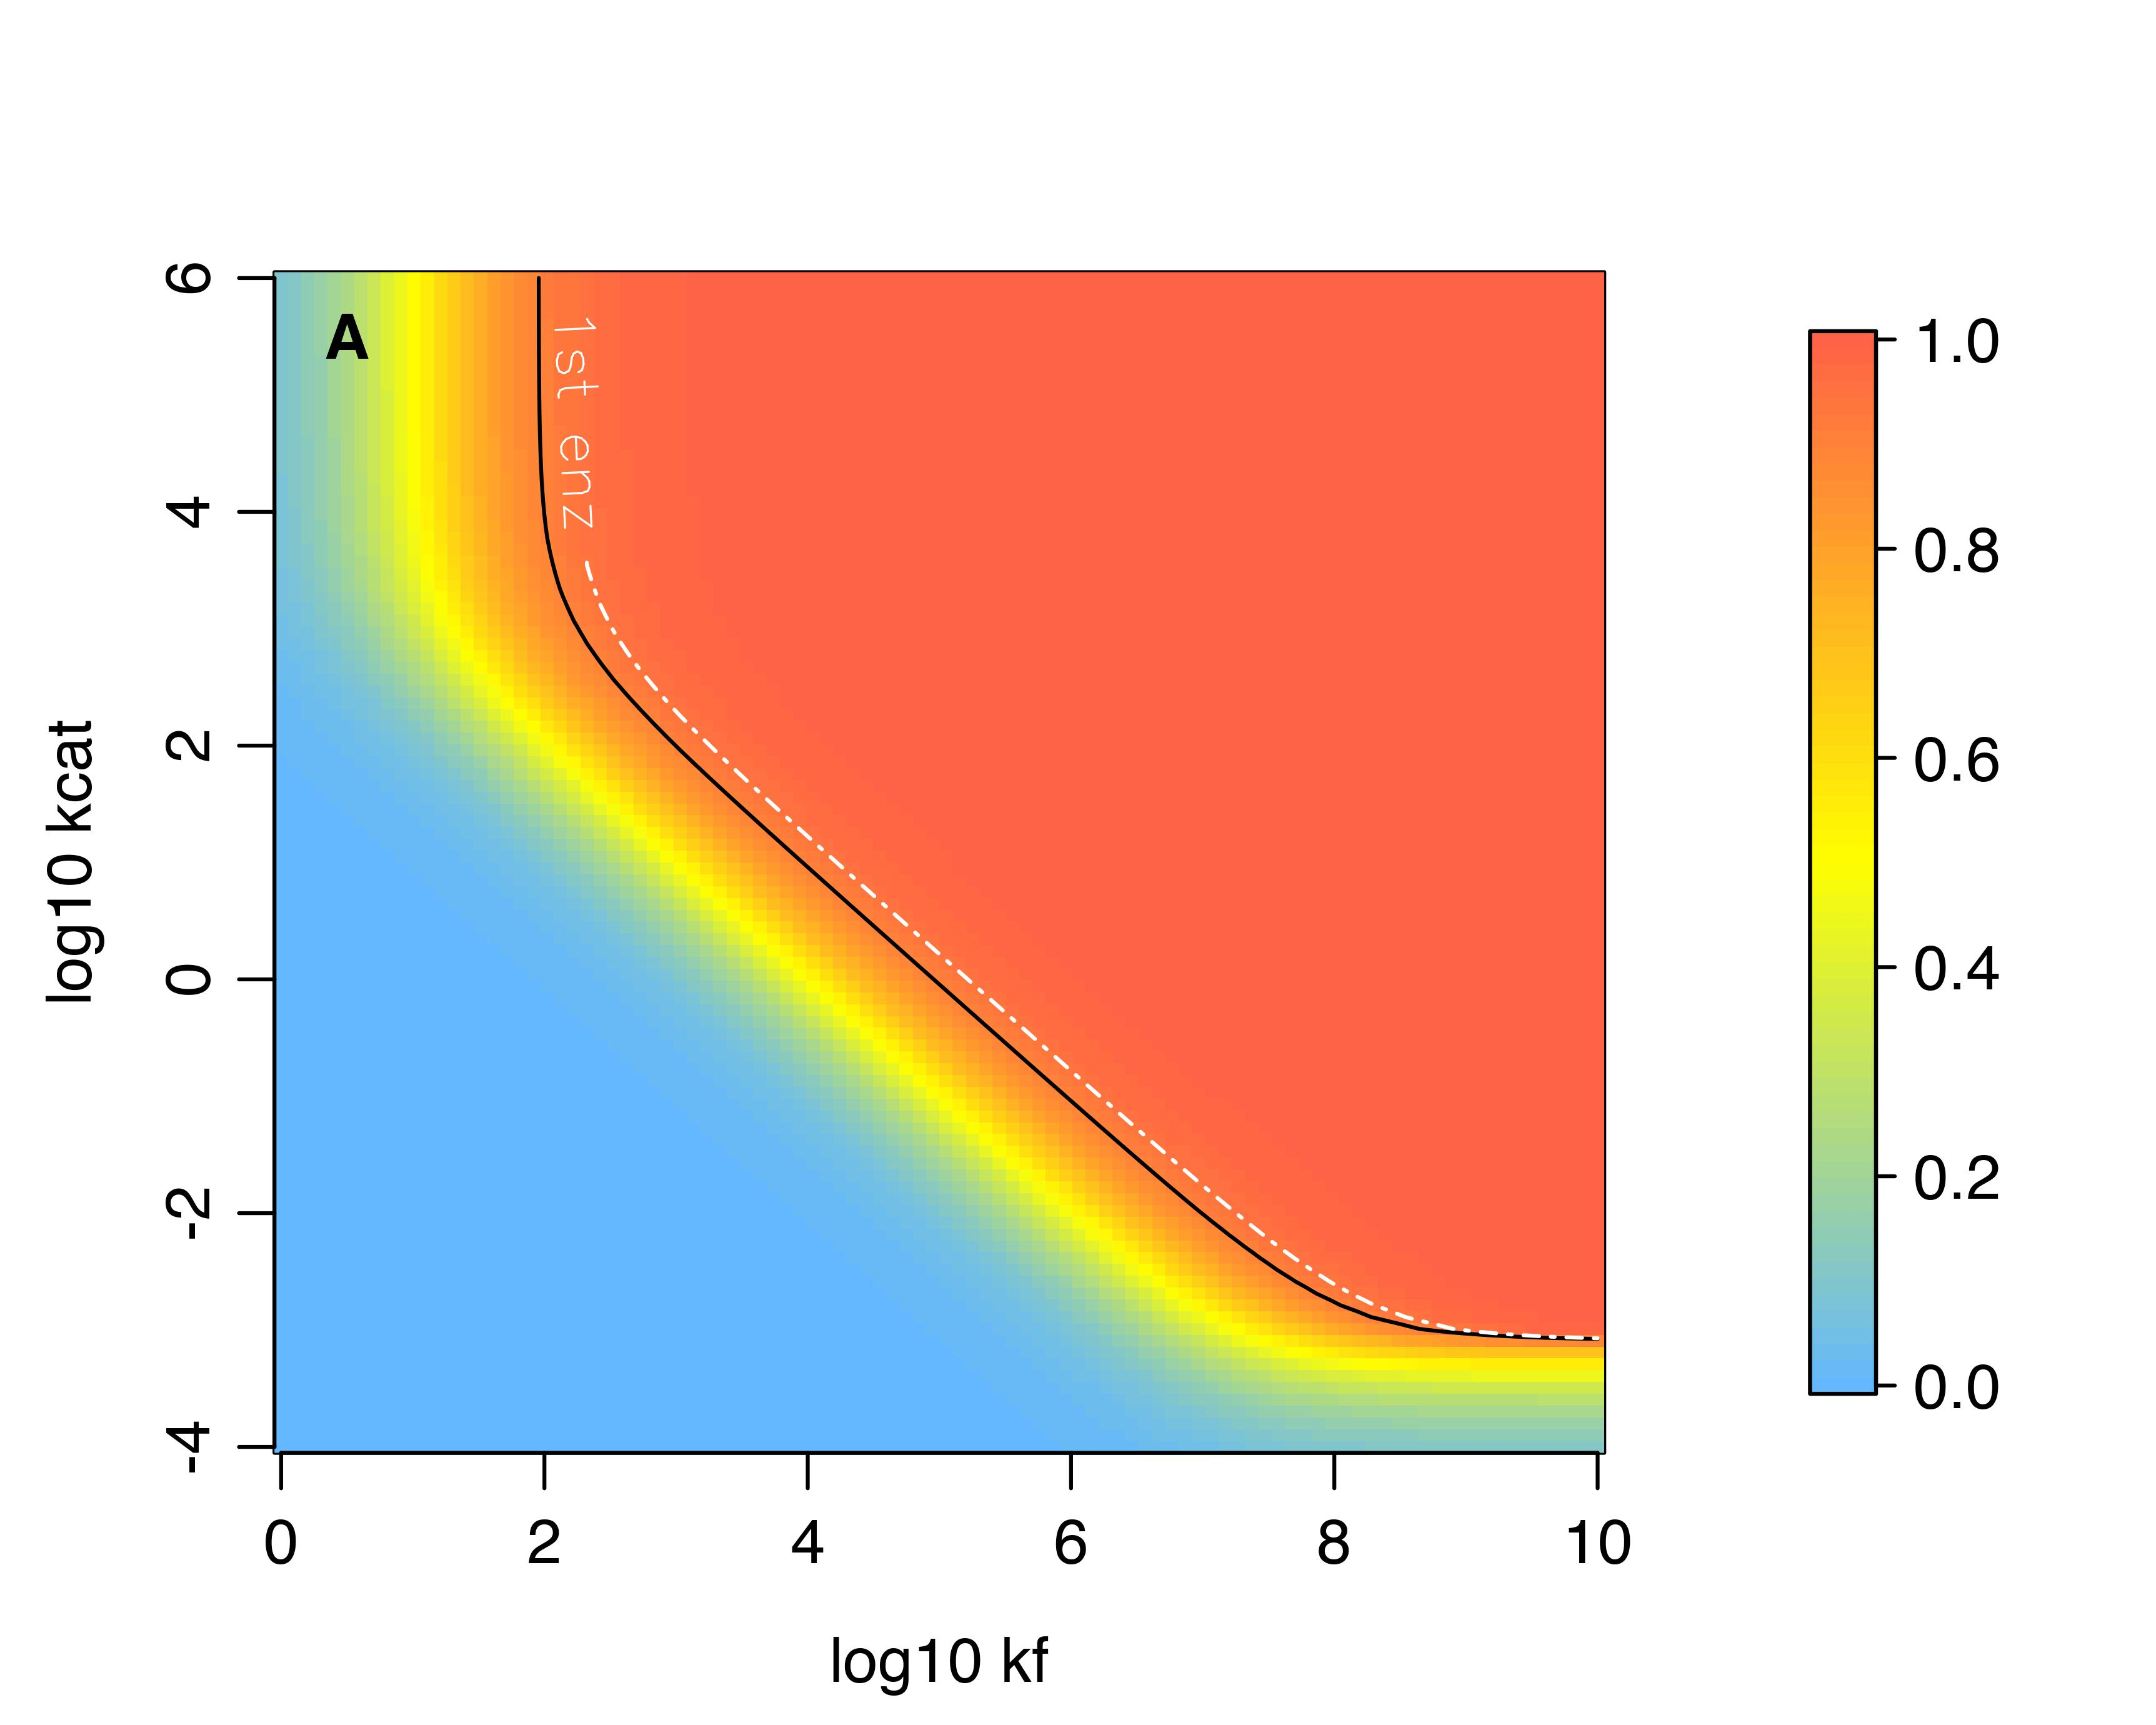
\includegraphics[scale=0.5]{Figures/2DFitLandscape_etahigh_noreverse.png} 
\end{minipage} \hfill
\begin{minipage}[c]{0.48\linewidth}
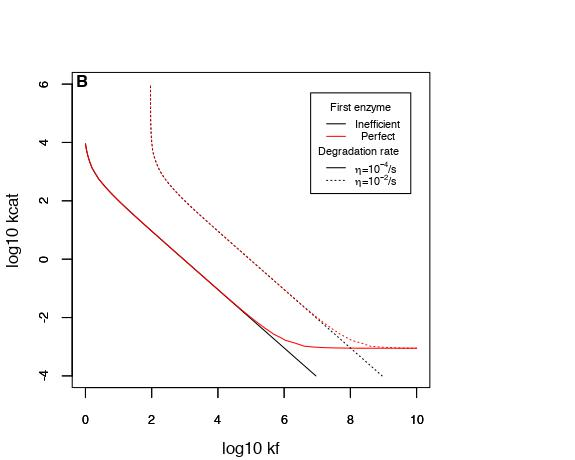
\includegraphics[scale=0.65,trim=0cm 0cm 0cm 1.5cm,clip]{Figures/2DFit_Landscape_2Enz_First_Enz_Influence.jpeg} 
\end{minipage}
\caption{Downstream enzymes exhibit similar fitness landscapes as \DIFaddbeginFL \DIFaddFL{those }\DIFaddendFL upstream, with a dependency to degradation parameter $\eta_d$. \DIFdelbeginFL \DIFdelFL{These enzymes are involved in a moderate flux pathway whose pace is driven by the same uptake kinetics as in FIG.~\ref{figure3D2DFit} where $\displaystyle V_{Tm}=1 \mu M/s$, $\displaystyle K_T=50\mu M$ and $\displaystyle [S_\text{out}]=10K_T$. Settings for the second enzyme also correspond to a model case with $k_r=1000s^{-1}$ and $ [E_{tot}]=1mM$. (}\DIFdelendFL A\DIFdelbeginFL \DIFdelFL{) corresponds to }\DIFdelendFL \DIFaddbeginFL \DIFaddFL{: }\DIFaddendFL a high degradation rate \DIFdelbeginFL \DIFdelFL{$\eta_{d}=10^{-1}s^{-1}$ that limits metabolite intracellular concentration to $[S]_{in}=10\mu M$ }\DIFdelendFL (\DIFdelbeginFL \DIFdelFL{for the selected $V_{Tm}$ value}\DIFdelendFL \DIFaddbeginFL \DIFaddFL{$\eta_d=10^{-2} /s$}\DIFaddendFL ) \DIFdelbeginFL \DIFdelFL{, with the upstream enzyme being perfect and concentrated ($k_f=10^{10}M^{-1}.s^{-1}$, $k_{cat}=10^6s^{-1}$, $k_r=10^3s^{-1}$, $[E_{tot}]=1mM$) and }\DIFdelendFL results in a fitness \DIFdelbeginFL \DIFdelFL{landscape }\DIFdelendFL \DIFaddbeginFL \DIFaddFL{plateau for the second enzyme }\DIFaddendFL very similar to that of the first enzyme \DIFdelbeginFL \DIFdelFL{when it faces similar conditions (findings are relatively similar for sugar like transporters, as reported }\DIFdelendFL \DIFaddbeginFL \DIFaddFL{; }\DIFaddendFL in \DIFdelbeginFL \DIFdelFL{SM - Figure S4), while plateau isoclines drawn }\DIFdelendFL \DIFaddbeginFL \DIFaddFL{the case presented the first enzyme is considered ``perfect'' }\DIFaddendFL in \DIFdelbeginFL \DIFdelFL{(B) also show results for a second degradation rate limiting this concentration }\DIFdelendFL \DIFaddbeginFL \DIFaddFL{order }\DIFaddendFL to \DIFdelbeginFL \DIFdelFL{$[S]_{in}=10mM$, in }\DIFdelendFL \DIFaddbeginFL \DIFaddFL{draw }\DIFaddendFL the \DIFdelbeginFL \DIFdelFL{context }\DIFdelendFL \DIFaddbeginFL \DIFaddFL{fitness landscape }\DIFaddendFL of \DIFdelbeginFL \DIFdelFL{an upstream concentrated }\DIFdelendFL \DIFaddbeginFL \DIFaddFL{the second }\DIFaddendFL enzyme \DIFdelbeginFL \DIFdelFL{being either perfect }\DIFdelendFL (\DIFdelbeginFL \DIFdelFL{see above}\DIFdelendFL \DIFaddbeginFL \DIFaddFL{$k_f=10^{10}M^{-1}.s^{-1}$, $k_{cat}=10^6s^{-1}$, $k_r=10^3s^{-1}$, $[E_{tot}]=1mM$}\DIFaddendFL )\DIFaddbeginFL \DIFaddFL{. B: decreasing the degradation rate allows less efficient enzymes (with lower $k_\text{cat}$ }\DIFaddendFL or \DIFaddbeginFL \DIFaddFL{$k_f$) to reach the fitness plateau. Considering the first enzyme to be }\DIFaddendFL inefficient ($k_f=10^{2}M^{-1}.s^{-1}$, $k_{cat}=10^{-2}s^{-1}$, $k_r=10^3s^{-1}$) \DIFdelbeginFL \DIFdelFL{. Decreasing $\eta_d$ makes }\DIFdelendFL \DIFaddbeginFL \DIFaddFL{instead of perfect marginally changes }\DIFaddendFL the \DIFdelbeginFL \DIFdelFL{cell }\DIFdelendFL \DIFaddbeginFL \DIFaddFL{fitness landscape by making organisms }\DIFaddendFL tolerant to \DIFdelbeginFL \DIFdelFL{higher concentrations of intermediate metabolites }\DIFdelendFL \DIFaddbeginFL \DIFaddFL{extremely low $k_\text{cat}$. Other parameter values are identical to FIG.~\ref{figure3D2DFit} }\DIFaddendFL (\DIFdelbeginFL \DIFdelFL{the product of the first reaction)}\DIFdelendFL \DIFaddbeginFL \DIFaddFL{findings are relatively similar for sugar-like transporters}\DIFaddendFL , \DIFdelbeginFL \DIFdelFL{hence relieving the selection pressure on the second enzyme and moving the plateau towards the bottomleft corner}\DIFdelendFL \DIFaddbeginFL \DIFaddFL{as reported in SM - Fig}\DIFaddendFL . \DIFaddbeginFL \DIFaddFL{S6).}\DIFaddendFL }
\label{figure2D_2Enz_Deg}
\end{figure*}

\DIFdelbegin \DIFdel{In this section, we intend to draw fitness landscapes for enzymes catalysing reactions downstream in }\DIFdelend \DIFaddbegin \DIFadd{One of the factors that makes enzymes different along a pathway is their position, such that the fitness landscape in FIG.\ref{figure3D2DFit} may only hold for the most upstream enzyme in a pathway. Indeed, because }\DIFaddend the \DIFdelbegin \DIFdel{metabolic pathway. Because the }\DIFdelend flux of the first product in a pathway increases with the substrate gradient across the cell membrane, the upstream enzyme of a given metabolic pathway is selected for efficiency \DIFdelbegin \DIFdel{within the limits mentioned in the previous two sections}\DIFdelend \DIFaddbegin \DIFadd{as described above}\DIFaddend . In contrast, this \DIFdelbegin \DIFdel{selective }\DIFdelend \DIFaddbegin \DIFadd{selection }\DIFaddend pressure does not apply directly downstream; at steady-state, even inefficient enzymes can in principle process newly formed substrate molecules at an elevated rate, assuming that the concentration of the substrate is allowed to reach any \DIFdelbegin \DIFdel{equilibrium }\DIFdelend \DIFaddbegin \DIFadd{steady-state }\DIFaddend value. This is an obviously unreasonable assumption, since a part of this standing substrate should be lost by outward diffusion or degradation \DIFdelbegin \DIFdel{, or may interfere with other cellular processes due to the surging involvement in non-specific or promiscuous interactions \citep{Khersonsky10,Schauble13}. We included a degradation term in the model, proportional to the constant }\DIFdelend \DIFaddbegin \DIFadd{\citep{Jones15,Bosdriesz18}. The loss of fitness may therefore result from the loss of metabolites in a way that can be modelled by a constant degradation rate }\DIFaddend $\eta_{d}$ \DIFaddbegin \DIFadd{\citep{Chou14} }\DIFaddend (assuming that the external environment is infinite, the degradation term can as well represent an efflux). \DIFdelbegin \DIFdel{Modelling the cost of accumulation this way is likely also consistent with }\DIFdelend \DIFaddbegin \DIFadd{Highly concentrated metabolites may also be involved in widespread }\DIFaddend non-specific \DIFaddbegin \DIFadd{\citep{Keller15} or promiscuous interactions \citep{Khersonsky10,Schauble13,Peracchi18} that may interfere with other cellular processes; this is well captured by the linear cost as non-specific }\DIFaddend interactions \DIFdelbegin \DIFdel{that }\DIFdelend should follow Michaelis-Menten kinetics albeit with much lower affinities\DIFdelbegin \DIFdel{and rates than the focal reaction, which means their rates should follow a }\DIFdelend \DIFaddbegin \DIFadd{, hence following an approximately }\DIFaddend linear relationship up to very high cellular concentrations \DIFdelbegin \DIFdel{.
}\DIFdelend \DIFaddbegin \DIFadd{(see Materials and Methods for more details). However for some reactions the accumulation of metabolites may result in the production of toxic compounds \citep{Lilja17, Niehaus20}, hence triggering toxicity best modelled as a non-linear fitness cost \citep{Clark91,Wright10}.
}\DIFaddend 

We first consider a ``perfect", highly concentrated upstream enzyme ($k_f=10^{10}M^{-1}s^{-1}$, $k_{cat}=10^6s^{-1}$, $k_r=10^3s^{-1}$, $[E_{tot}]=10^{-3}M$) and \DIFdelbegin \DIFdel{study }\DIFdelend \DIFaddbegin \DIFadd{focus on }\DIFaddend the second enzyme in the pathway, showing that it evolves on a fitness landscape that has a similar shape than described above, still hitting a plateau (FIG.~\ref{figure2D_2Enz_Deg}, with the same parameterization as FIG.~\ref{figure3D2DFit}). The degradation rate creates a ceiling for the concentration of the product of the first reaction, such that reducing $\eta_{d}$ allows for higher concentrations (see SM \DIFdelbegin \DIFdel{- Figure S3}\DIFdelend \DIFaddbegin \DIFadd{Fig. S4}\DIFaddend ) and makes the flux tolerant to second enzymes with lower $k_f$s, whereas selection on $k_\text{cat}$ is barely impacted by this parameter. The plateau is therefore extended to the left when high product concentrations are enabled at low $\eta_{d}$ (see FIG.~\ref{figure2D_2Enz_Deg}-B). The shape of the plateau is little impacted by changes in the efficiency of the first enzyme, especially when it stands on the plateau. These \DIFdelbegin \DIFdel{conclusions are independent of characteristics of }\DIFdelend \DIFaddbegin \DIFadd{results are almost independent of }\DIFaddend the transporter initiating the pathway 
\DIFdelbegin \DIFdel{, although degradation rates limiting metabolite concentrations to similar levels pushes the plateau to the right slightly more when compared to the landscape of the first enzyme }\DIFdelend (see SM \DIFdelbegin \DIFdel{- Figure S4 }\DIFdelend \DIFaddbegin \DIFadd{Fig. S6 }\DIFaddend for the case of \DIFdelbegin \DIFdel{low affinity- }\DIFdelend \DIFaddbegin \DIFadd{moderate affinity, }\DIFaddend high flux transporters). 
\DIFdelbegin \DIFdel{We can notice that the second enzyme 's kinetic parameters evolve in response to the net rate $v$ of the upstream reaction and to the presence of any process in competition for its product (like efflux or degradation) , such that these results are expected to hold for any enzyme downstream. 
}\DIFdelend 

\DIFdelbegin \subsection{\DIFdel{Most enzymes lie on the fitness plateau}}
%DIFAUXCMD
\addtocounter{subsection}{-1}%DIFAUXCMD
%DIFDELCMD < 

%DIFDELCMD < \begin{figure*}[h!]
%DIFDELCMD < \centering
%DIFDELCMD < \includegraphics[scale=0.43,trim=0cm -0.75cm 0cm 1.5cm,clip]{Figures/2DFitLandscape_Full_Dataset.jpeg}
%DIFDELCMD < %%%
\DIFdelFL{\hspace{-0.3cm}
}%DIFDELCMD < 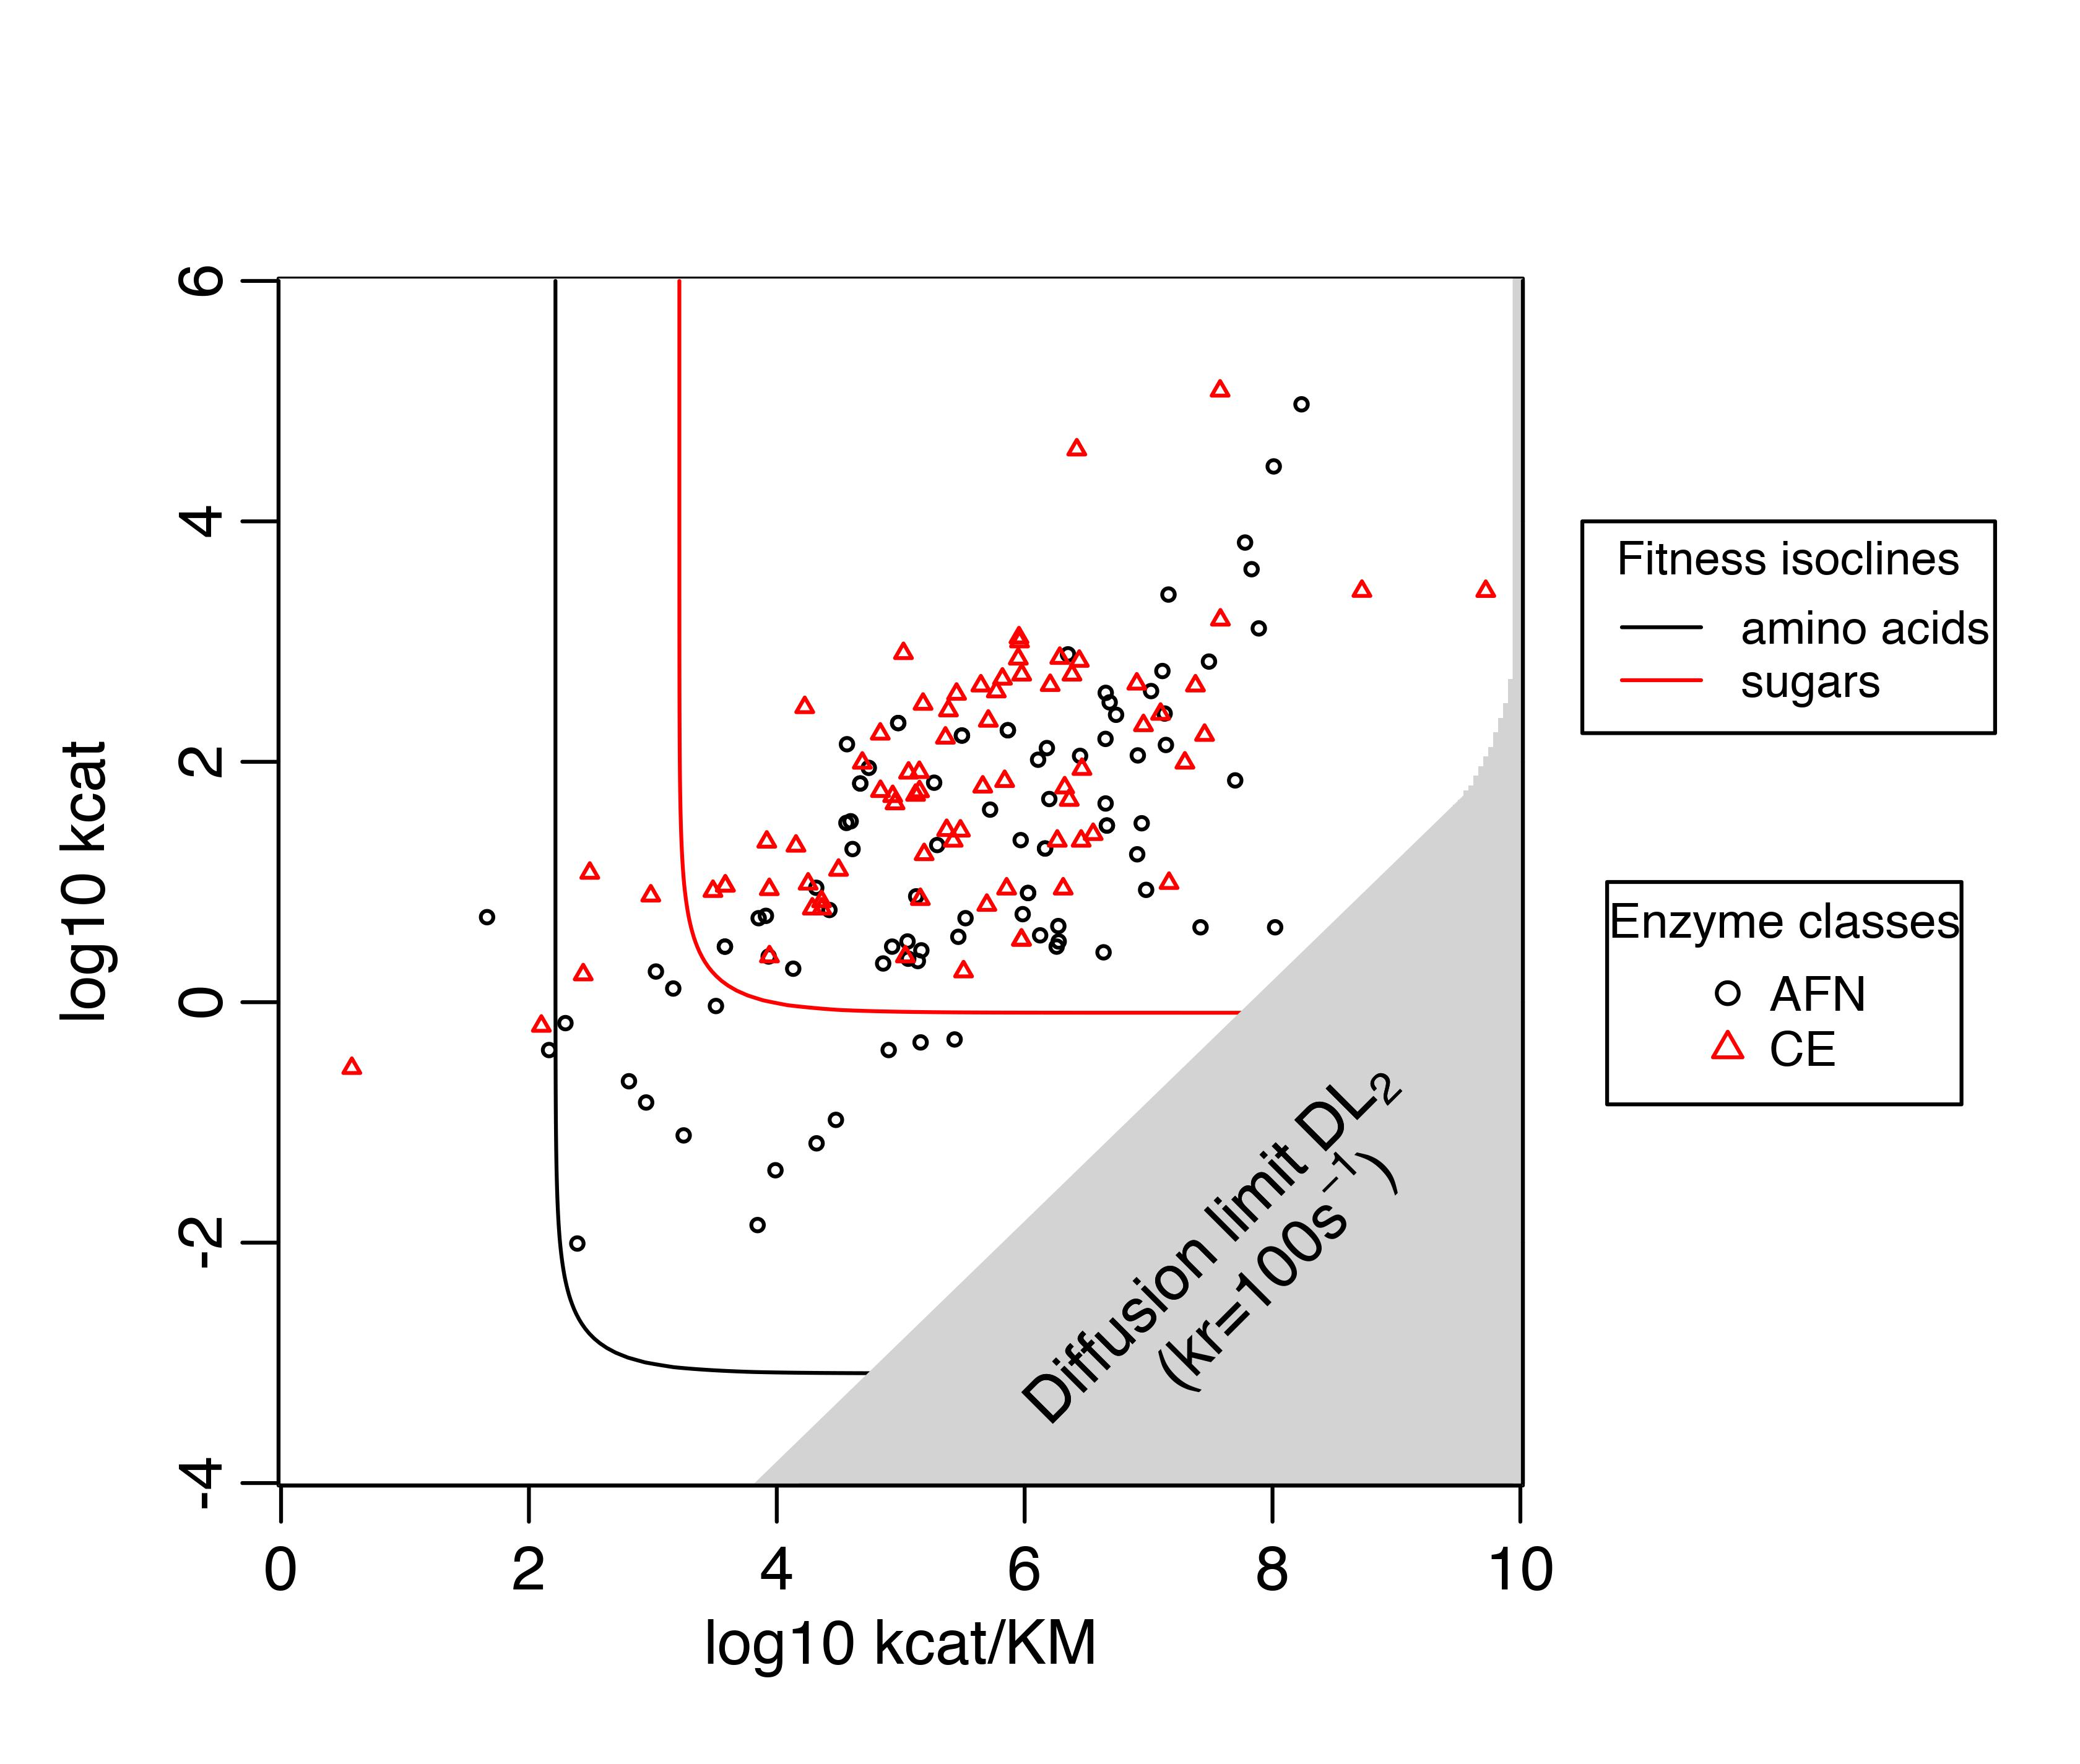
\includegraphics[scale=0.43,trim=0cm -0.75cm 0cm 1.5cm,clip]{Figures/2DFitContour_DataClasses.jpeg}  
%DIFDELCMD < %%%
%DIFDELCMD < \caption{%
{%DIFAUXCMD
\DIFdelFL{\textit{in vitro} experimental estimates for enzyme kinetic parameters spread on the plateau of a generic theoretical fitness landscape. The parameter space considered corresponds to the usual empirical estimates for enzyme kinetic parameters $k_\text{cat}$ and $k{cat}/K_M$. The space is narrowed down here due to the diffusion limit, outlined by the grey area when $k_r$ is low ($10^2s^{-1}$), that impedes high values for $k_{cat}/K_M$ under low values for the ratio between $k_{cat}$ and $k_r$. In (A), the full dataset from \citep{Bar-Even11} is plotted in the parameter space and contrasted with the fitness landscape of the most upstream enzyme involved in amino acid or nucleoside metabolism (same parameters for transport than in Fig.~\ref{figure3D2DFit}, $[E_{tot}]=10^{-3}M$ and $k_r=10^{2}s^{-1}$). Most enzymes fall on the plateau of the fitness landscape. A few outliers overcome the diffusion limit, suggesting that $k_r$ might be lower than $10^2s^{-1}$ for these enzymes. In (B), the dataset is divided into classes identified by \citet{Bar-Even11}, with the acronym denoting enzymes involved in the central metabolism including (AFN): amino acids, fatty acids, and nucleotides  - and (CE): carbohydrates and energy. The isoclines shown correspond to parameter values typical of sugar transporters ($K_T=5mM$,$V_{Tm}=1mM.s^{-1}$) \citep{Maier02} or amino acids transporters (same as in (A)). With a few exceptions, enzymes seem to spread on the corresponding fitness plateau.}}
%DIFAUXCMD
%DIFDELCMD < \label{figure2D_BarEven_Dataset}
%DIFDELCMD < \end{figure*}
%DIFDELCMD < 

%DIFDELCMD < %%%
\DIFdel{We then superimposed empirical estimates of kinetic parameters over our theoretical fitness landscapes, after substituting parameter }\DIFdelend \DIFaddbegin \DIFadd{The shape of the negative relationship between metabolite concentration and fitness can be important (Figs~S7-S9 in SM), as it can make the fitness landscape of an enzyme dependent of the overall flux of the metabolic pathway, and therefore on other enzymes in the pathway. Indeed, low general fluxes (as modelled by an inefficient first enzyme in Figs. S7-S8) make the metabolite concentration below its toxicity threshold, therefore making organisms tolerant to enzymes with lower }\DIFaddend $k_f$ \DIFdelbegin \DIFdel{for its usual empirical counterpart, $k_\text{cat} / K_M$. Because $k_{cat}/K_M \approx k_fk_{cat}/k_r$, this approximation only holds when $k_\text{cat} \gg k_r$. No less significantly, representing the fitness landscape in this parameter space
sets an area in the bottomright part of the landscapes where $k_f$ exceeds the diffusion limit (grey area on FIG. ~\ref{figure2D_BarEven_Dataset}) . For purposes of inclusiveness, we used $k_r=10^{2}s^{-1}$ by default -- noting that this limit would be displaced upwards for larger $k_r$ -- and otherwise used the same set of parameters as in FIG. ~\ref{figure3D2DFit} to obtain FIG.~\ref{figure2D_BarEven_Dataset}. We see that a vast majority of the enzymes in the \citet{Bar-Even11} dataset belong to the fitness plateau. 
The implicit suggestion that this could be a result of Evolution on a common fitness landscape is surprising, as the dataset includes enzymes from many Eukaryote and Prokaryote species that contribute to various pathways. We instead anticipate that differences in evolutionary context should explain a part of the observed variance. We also note a strong linear positive relationship between $k_{cat}$ }\DIFdelend and \DIFdelbegin \DIFdel{$k_{cat}/K_M$ (\textbf{$R^2=0.4$}). This illustrates how focusing on $k_{cat}/K_M$ can be misleading if one's interest lies in mechanistic processes and their implications. Indeed, as obvious as it may sound, $k_{cat}$ and $k_{cat}/K_M$ are not independent from each other, especially when $k_\text{cat}<k_r$ (which is the case for a majority of the data points in FIG. \ref{figure2D_BarEven_Dataset}). Concluding on whether a positive relationship between }\DIFdelend \DIFaddbegin \DIFadd{$k_\text{cat}$. Taken together, these results show that the precise epistatic relationship between enzymes in a pathway will depend on the exact cost function applied, with a linear cost generating epistasis for $k_\text{cat}$ only and a non-linear cost possibly impacting both }\DIFaddend $k_f$ and \DIFdelbegin \DIFdel{$k_\text{cat}$ does exist would require to estimate $k_r$ for each enzyme.
}\DIFdelend \DIFaddbegin \DIFadd{$k_\text{cat}$. 
}\subsection{\DIFadd{The reversibility of reactions also matters}}
\DIFaddend 

\DIFdelbegin \DIFdel{Because we have previously shown that different transporters may yield plateaus with different shapes (\textit{e.g.} for sugars and amino acids) , our model predicts that enzymesinvolved in }\DIFdelend \DIFaddbegin \DIFadd{Reversibility is an intrinsic feature of chemical reactions that cannot be directly overcome by Evolution \citep{Haldane30,Cornish-Bowden79a}. A highly reversible reaction corresponds to a large intrinsic equilibrium constant $K_{eq}=[S]_{eq}/[P]_{eq}$ \citep{Klipp94}, and results in higher backward than forward rates in the following chemical equation: }\begin{equation}
\ce{ E + S <=>[k_{f}][k_{r}] ES <=>[k_{cat}][k_{inh}] E + P_1 }\DIFadd{,
\label{chemMM_fullrev}
}\end{equation}
\DIFadd{where $k_{inh}$ represents the rate at which enzyme and product combine back. Such a (reversible) reaction could in principle influence the selective pressure acting on the following enzyme in the pathway, for both enzymes compete to process the same metabolite $P_1$. We thus quantified how reversibility affects the evolution of an enzyme downstream (SM Figs S10 and S11). 
}

\DIFadd{The equilibrium constant $K_{eq}$ has a similar (non-linear) impact on the fitness landscape of the second enzyme to that of }\DIFaddend the \DIFdelbegin \DIFdel{corresponding pathways should have their own specific distributions. Representing findings by  \citep{Bar-Even11} suggests that there may indeed be an explainable difference between enzymes contributing to carbohydrate processing (in red in FIG.~\ref{figure2D_BarEven_Dataset}-B) and to that of amino acids (a part of the black dots in FIG.~\ref{figure2D_BarEven_Dataset}-B). %DIF < But, as we shall nevertheless emphasise, a proper analysis should include many other variables that may also contribute to the variance between enzymes.
This apparent discrepancy in fitness landscapes across pathways starting with different transporters can only explain a small part of the wide distribution of kinetic parameters reported by \citet{Bar-Even11}, thus requiring a careful study of other evolutionary, ecological and chemical parameters}\DIFdelend \DIFaddbegin \DIFadd{degradation rate, with a highly reversible upstream enzyme exerting a selection pressure downstream towards an increase of kinetic parameters (SM Fig. S10-A). Indeed, increasing $K_{eq}$ moves the fitness plateau toward the upper-right corner in the ($k_f$, $k_\text{cat}$) parameter space, hence selecting for more efficient downstream enzymes. The effect appears linear, except for very low values of $K_{eq}$ where metabolite accumulation exerts a dominant role in shaping the fitness landscape (through the degradation rate $\eta_d$, set to a low residual value). Therefore, the reversibility of the upstream reaction appears like a critical parameter for the evolution of an enzyme}\DIFaddend . 


\subsection{Evolutionary dynamics of enzyme kinetic parameters}

\begin{figure*}[h!]
\centering
\DIFdelbeginFL %DIFDELCMD < \begin{minipage}[c]{0.48\linewidth}
%DIFDELCMD < \includegraphics[scale=0.64,trim=0cm 0cm 3cm 1.5cm,clip]{Figures/2DFitLandscape_Evo_Results_lowF_nobias.jpeg}
%DIFDELCMD < %%%
\DIFdelendFL \DIFaddbeginFL \begin{minipage}[c]{0.5\linewidth}
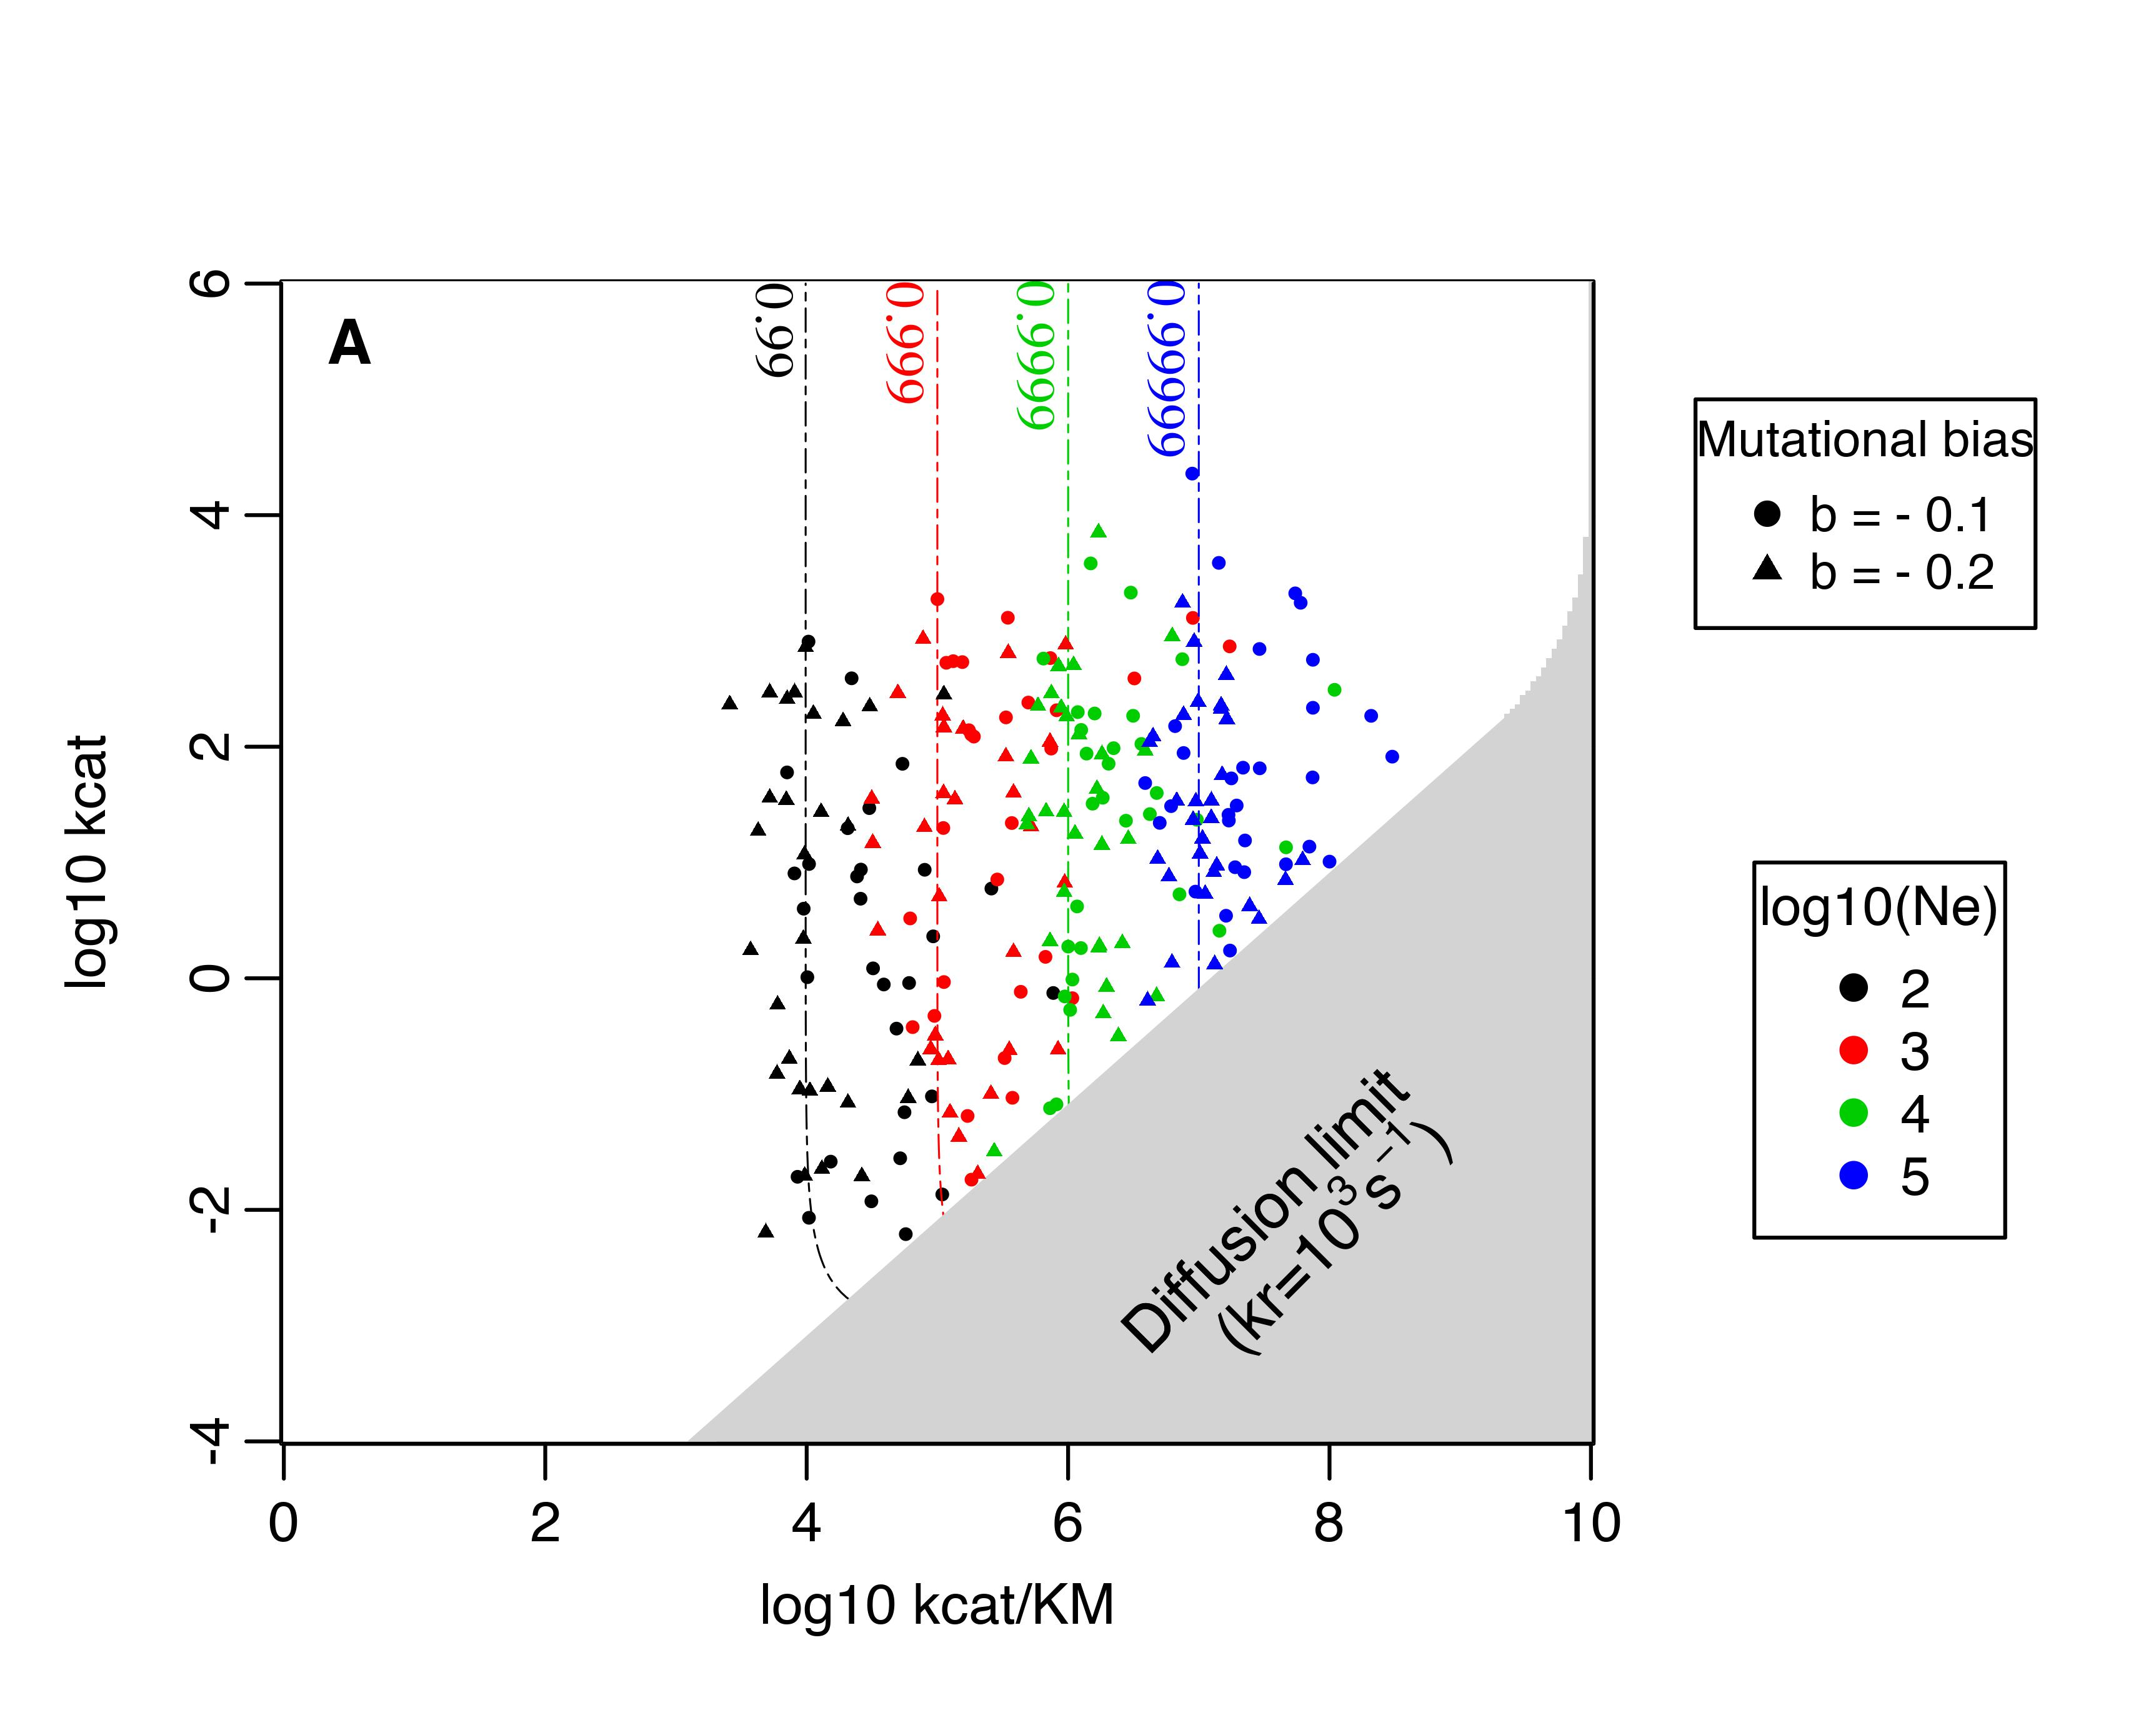
\includegraphics[scale=0.65,trim=0.25cm 0cm 0.5cm 1.5cm,clip]{Figures/2DFitLandscape_Evo_Results_lowF_withbias_Def.jpeg} 
\DIFaddendFL \end{minipage} \DIFdelbeginFL \DIFdelFL{\hspace{-0.5cm}%DIF < \hfill
}%DIFDELCMD < \begin{minipage}[c]{0.48\linewidth}
%DIFDELCMD < \includegraphics[scale=0.64,trim=1cm 0cm 0.5cm 1.5cm,clip]{Figures/2DFitLandscape_Evo_Results_lowF_withbias.jpeg} 
%DIFDELCMD < %%%
\DIFdelendFL \DIFaddbeginFL \DIFaddFL{\hspace{0.5cm}}\hfill
\begin{minipage}[c]{0.46\linewidth}
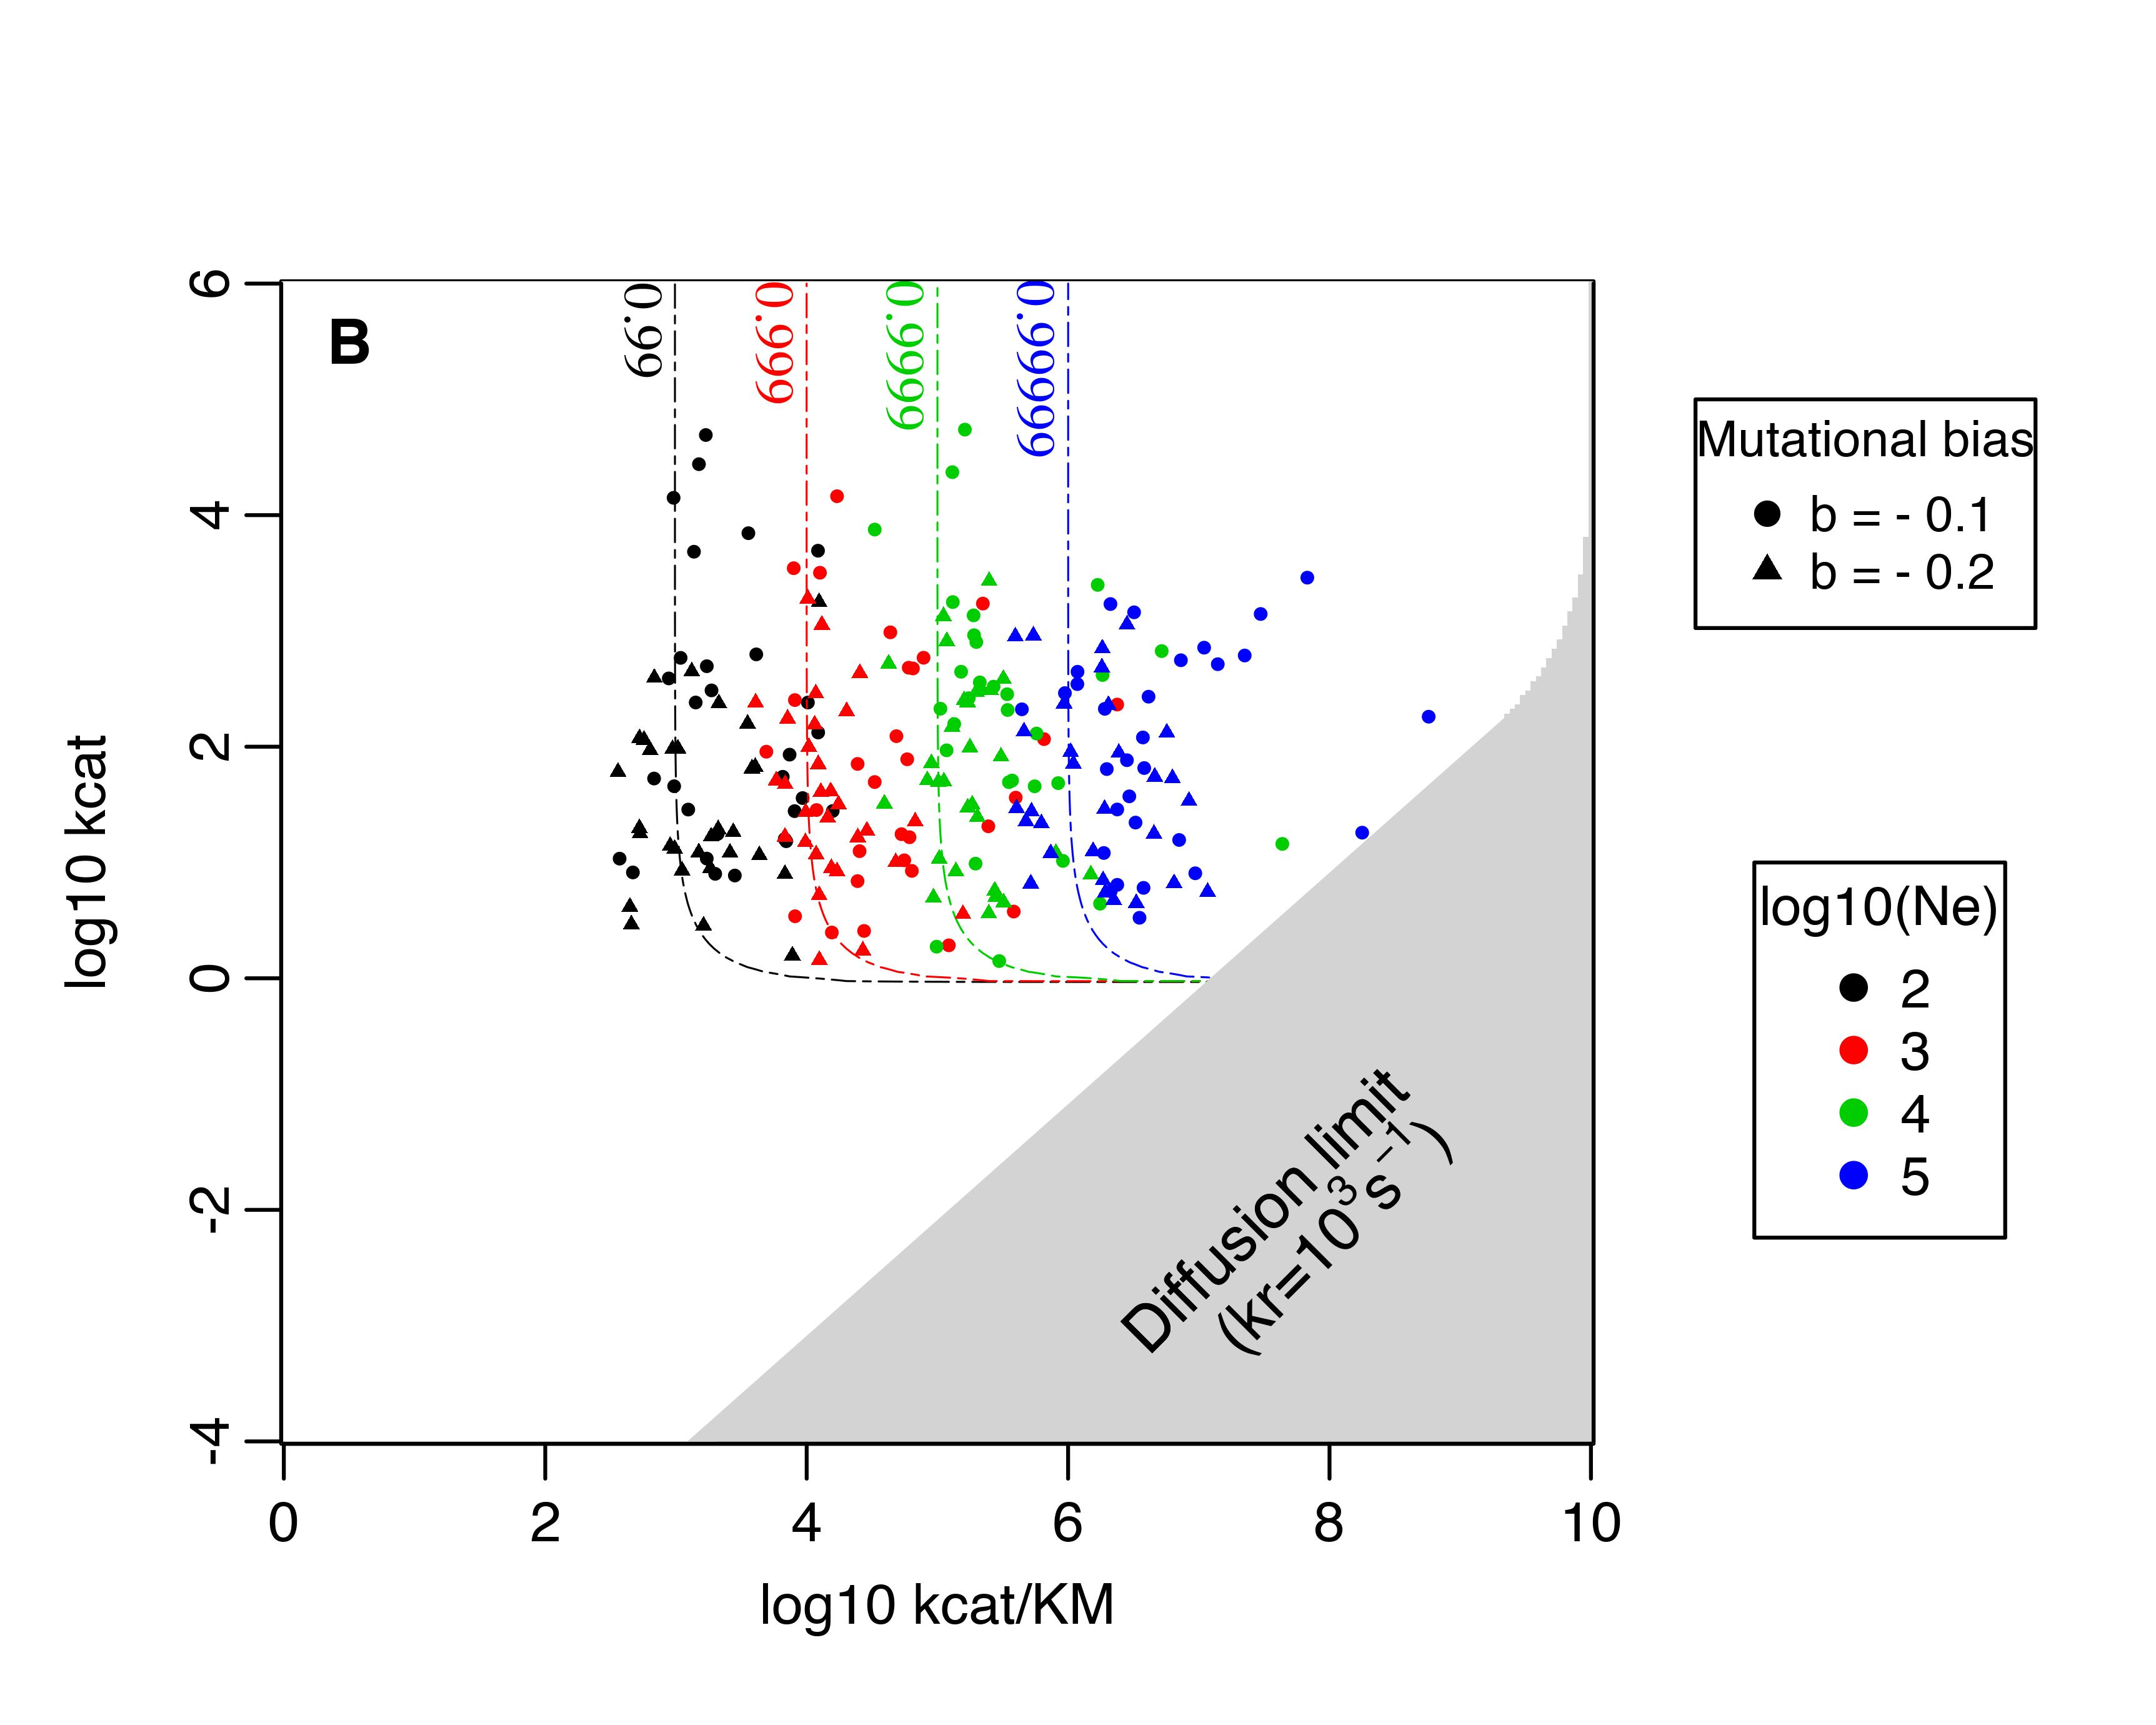
\includegraphics[scale=0.65,trim=0cm 0cm 3.5cm 1.5cm,clip]{Figures/2DFitLandscape_Evo_Results_highF_withbias_Def.jpeg} 
\DIFaddendFL \end{minipage}
\caption{\DIFdelbeginFL \DIFdelFL{Simulations of a population genetics model indicate }\DIFdelendFL \DIFaddbeginFL \DIFaddFL{Population genetic simulations predict }\DIFaddendFL that enzymes should \DIFdelbeginFL \DIFdelFL{spread on }\DIFdelendFL \DIFaddbeginFL \DIFaddFL{reach }\DIFaddendFL a \DIFdelbeginFL \DIFdelFL{plateau corresponding to their effective population size $N_e$ only }\DIFdelendFL \DIFaddbeginFL \DIFaddFL{predictable set of features }\DIFaddendFL when \DIFdelbeginFL \DIFdelFL{mutations are unbiased; mutations }\DIFdelendFL \DIFaddbeginFL \DIFaddFL{mutation }\DIFaddendFL biases towards lower efficiencies \DIFdelbeginFL \DIFdelFL{make enzymes stick to isoclines}\DIFdelendFL \DIFaddbeginFL \DIFaddFL{are considered (see SM  fig. S17 for the case of an absence of bias). Indeed}\DIFaddendFL , \DIFdelbeginFL \DIFdelFL{such }\DIFdelendFL \DIFaddbeginFL \DIFaddFL{the mutation selection drift equilibrium establishes close to an isocline indicative of effective selection }\DIFaddendFL that \DIFdelbeginFL \DIFdelFL{their evolution is predictable}\DIFdelendFL \DIFaddbeginFL \DIFaddFL{depends on the effective population size $N_e$}\DIFaddendFL . The \DIFdelbeginFL \DIFdelFL{case }\DIFdelendFL \DIFaddbeginFL \DIFaddFL{cases }\DIFaddendFL considered here \DIFdelbeginFL \DIFdelFL{is }\DIFdelendFL \DIFaddbeginFL \DIFaddFL{are }\DIFaddendFL that of a transporter with a low flux at saturation and high affinity (\DIFaddbeginFL \DIFaddFL{A; }\DIFaddendFL $V_{Tm}=1\mu Ms^{-1}$ and $K_T=10\mu M$) \DIFdelbeginFL \DIFdelFL{-- under various scenarios: four }\DIFdelendFL \DIFaddbeginFL \DIFaddFL{and one with a high flux at saturation but low affinity (B; $V_{Tm}=1mMs^{-1}$ and $K_T=100mM$) with }\DIFaddendFL effective population sizes \DIFaddbeginFL \DIFaddFL{ranging }\DIFaddendFL from $10^2$ to $10^5$ (different colors) and \DIFdelbeginFL \DIFdelFL{three cases }\DIFdelendFL \DIFaddbeginFL \DIFaddFL{two strengths }\DIFaddendFL of \DIFaddbeginFL \DIFaddFL{the }\DIFaddendFL mutational \DIFdelbeginFL \DIFdelFL{biases}\DIFdelendFL \DIFaddbeginFL \DIFaddFL{bias }\DIFaddendFL (\DIFdelbeginFL \DIFdelFL{($b=0$ corresponds to }\DIFdelendFL the absence of mutational bias \DIFaddbeginFL \DIFaddFL{was also considered, see SM}\DIFaddendFL ). \DIFdelbeginFL \DIFdelFL{We ran }\DIFdelendFL \DIFaddbeginFL \DIFaddFL{Each of }\DIFaddendFL 30 independent simulations for each scenario \DIFdelbeginFL \DIFdelFL{, each }\DIFdelendFL \DIFaddbeginFL \DIFaddFL{is }\DIFaddendFL represented a dot in the ``empirical" parameter space ($k_\text{cat}, \;k_\text{cat}/K_M$)\DIFdelbeginFL \DIFdelFL{. Only }\DIFdelendFL \DIFaddbeginFL \DIFaddFL{, but only }\DIFaddendFL $k_\text{cat}$ and $k_f$ were susceptible to evolve\DIFdelbeginFL \DIFdelFL{, while }\DIFdelendFL \DIFaddbeginFL \DIFaddFL{. }\DIFaddendFL $k_r$ \DIFdelbeginFL \DIFdelFL{was }\DIFdelendFL \DIFaddbeginFL \DIFaddFL{is }\DIFaddendFL set to $10^3s^{-1}$ such that the grey part of the parameter space is inaccessible to enzymes \DIFdelbeginFL \DIFdelFL{due to }\DIFdelendFL \DIFaddbeginFL \DIFaddFL{that would otherwise exceed }\DIFaddendFL the diffusion limit. 
\DIFdelbeginFL \DIFdelFL{At evolutionary equilibrium, enzyme efficiencies reach a plateau delineated by an isocline indicative of effective selection. In (A), no mutational bias results in enzymes spreading onto the plateau, some reaching very high $k_\text{cat}$ and/or $k_\text{cat}/K_M$ values, while in (B) enzyme efficiencies stick to their predicted isoclines -- under the Nearly Neutral Theory of Evolution \citep{Ohta92} -- owing to the over-representation of mutations reducing enzyme efficiencies.%DIF <  The stickiness is self-evidently correlated to the average mutational bias $b$.
}\DIFdelendFL }
\label{figure2D_Evolutionary_results}
\end{figure*}

\DIFaddbegin \DIFadd{How much variance in evolutionary outcomes these differences in fitness landscapes may explain is contingent on the interplay between selection, mutation and drift. Small differences in an isocline position should indeed be of little importance if populations perform random walks on the fitness plateau, for instance. }\DIFaddend To approach how populations evolve on \DIFdelbegin \DIFdel{the fitness landscapesdrawn through our mathematical model}\DIFdelend \DIFaddbegin \DIFadd{our mathematically derived fitness landscapes}\DIFaddend , we built a simple population genetics model \DIFdelbegin \DIFdel{that includes, besides selection, mutation and drift. In this individual based model, }\DIFdelend \DIFaddbegin \DIFadd{in which }\DIFaddend absolute fitness is directly proportional to the flux \DIFdelbegin \DIFdel{of product at equilibrium }\DIFdelend \DIFaddbegin \DIFadd{arising from the first enzyme at steady-state }\DIFaddend -- which itself equals the \DIFaddbegin \DIFadd{net }\DIFaddend inward flux of nutrients. \DIFdelbegin \DIFdel{We consider the flux of the first enzyme (see Methods and previous Results sections for details), as presumably the evolutionary dynamics should be similar for downstream enzymes with similar landscapes. }\DIFdelend Two different levels of metabolic demands were considered, corresponding to parameter values \DIFdelbegin \DIFdel{used to draw }\DIFdelend \DIFaddbegin \DIFadd{of amino acids/nucleosides and sugar transporters (}\DIFaddend panels (A) and (I) in \DIFdelbegin \DIFdel{FIG. ~\ref{figure2DSEns} in order to control that differences in the delineation of the plateau (in the parameter space)do not affect the evolutionary equilibrium. For the enzyme of a given individual}\DIFdelend \DIFaddbegin \DIFadd{SM Fig. S3). In this instance of the model}\DIFaddend , only $k_\text{cat}$ and $k_f$ were susceptible to evolve through mutations. Mutational effects on $\log_{10}k_{cat}$ and $\log_{10}k_f$ were drawn from independent normal distributions with mean $b \leq 0$, \DIFdelbegin \DIFdel{with }\DIFdelend \DIFaddbegin \DIFadd{and }\DIFaddend the absolute value of $b$ setting the intensity of \DIFdelbegin \DIFdel{mutational }\DIFdelend \DIFaddbegin \DIFadd{a mutational bias }\DIFaddend towards less efficient parameter values\DIFaddbegin \DIFadd{, as has been widely documented in many contexts \citep{EyreWalker07,Serohijos12,Heckmann18}}\DIFaddend . The standard deviation of the distribution of mutational effects \DIFdelbegin \DIFdel{was set to }\DIFdelend \DIFaddbegin \DIFadd{equals }\DIFaddend $0.3$ such that most mutations explore the neighbouring parameter space,  \DIFdelbegin \DIFdel{with rare mutations allowing changes }\DIFdelend \DIFaddbegin \DIFadd{seldom changing a parameter }\DIFaddend by more than one order of magnitude (one $\log_{10}$ unit) \DIFdelbegin \DIFdel{at a time, accordingly to values reported in \citep{Carlin16}. 
%DIF < Simulations were performed for Ne ranging from $10^2$ to $10^5$ individuals, and replicated 30 times for each set of parameter. (en matériel et méthodes, de toute façon on le voit avec les résultats)
}\DIFdelend \DIFaddbegin \DIFadd{in compliance with empirical estimates \citep{Carlin16}. Since the relation between kinetic parameters may be constrained -- \textit{e.g.} due to shared properties of the energy profile of a reaction -- we tested the influence of negative and positive relationships using bivariate normal distributions, with three different values of $\rho$ (see Materials and Methods for details). 
}\DIFaddend 

\DIFdelbegin %DIFDELCMD < \begin{figure*}[h!]
%DIFDELCMD < \centering
%DIFDELCMD < \begin{minipage}[c]{0.48\linewidth}
%DIFDELCMD < %%%
\DIFdelFL{\hspace{-1.3cm}
}%DIFDELCMD < 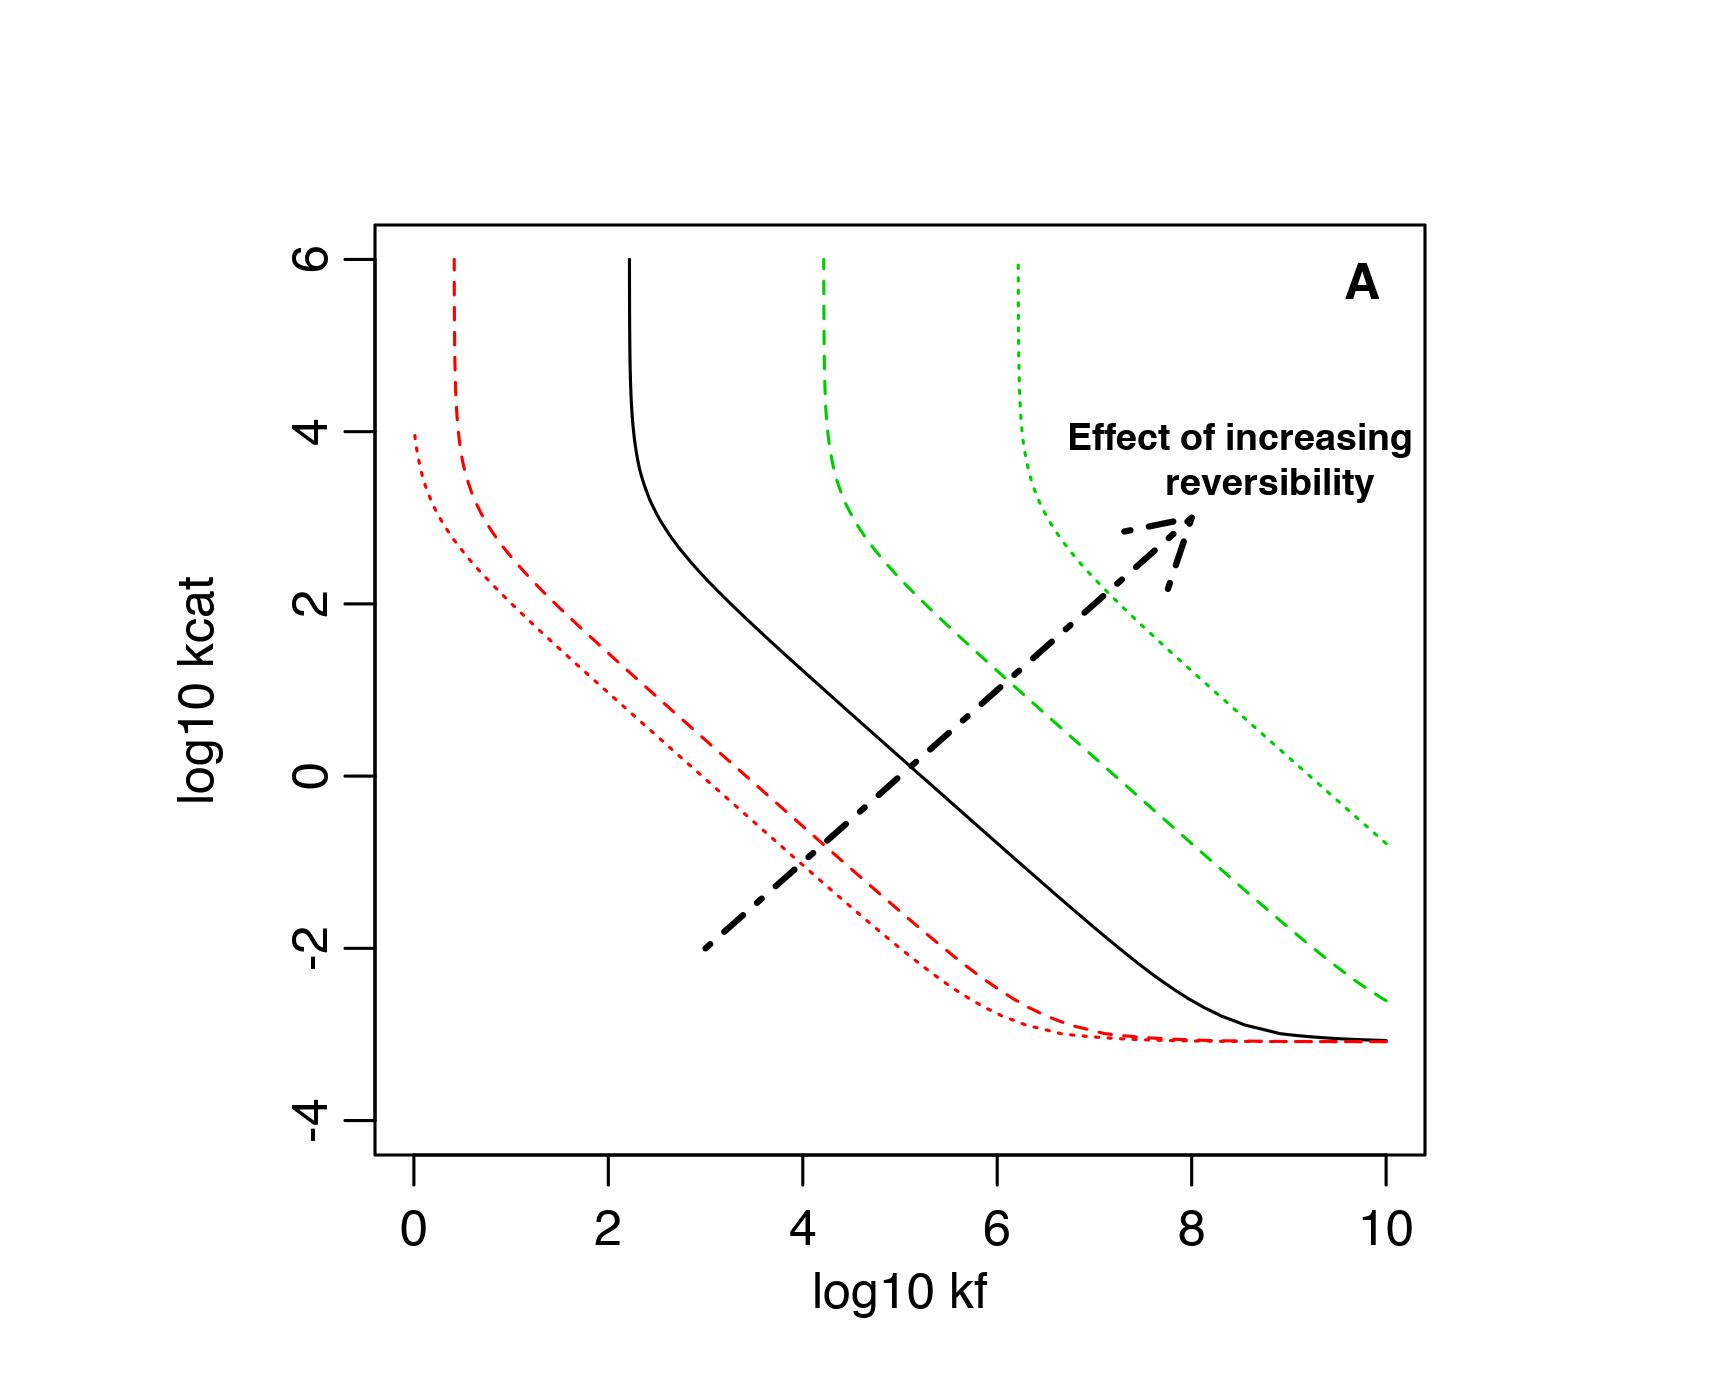
\includegraphics[scale=0.64,trim=0cm 0cm 0cm 1.5cm,clip]{Figures/2DFitLandscape_Multiple_Reverse.jpeg} 
%DIFDELCMD < \end{minipage} %%%
\DIFdelFL{\hspace{-1.3cm}
}%DIFDELCMD < \begin{minipage}[c]{0.48\linewidth}
%DIFDELCMD < 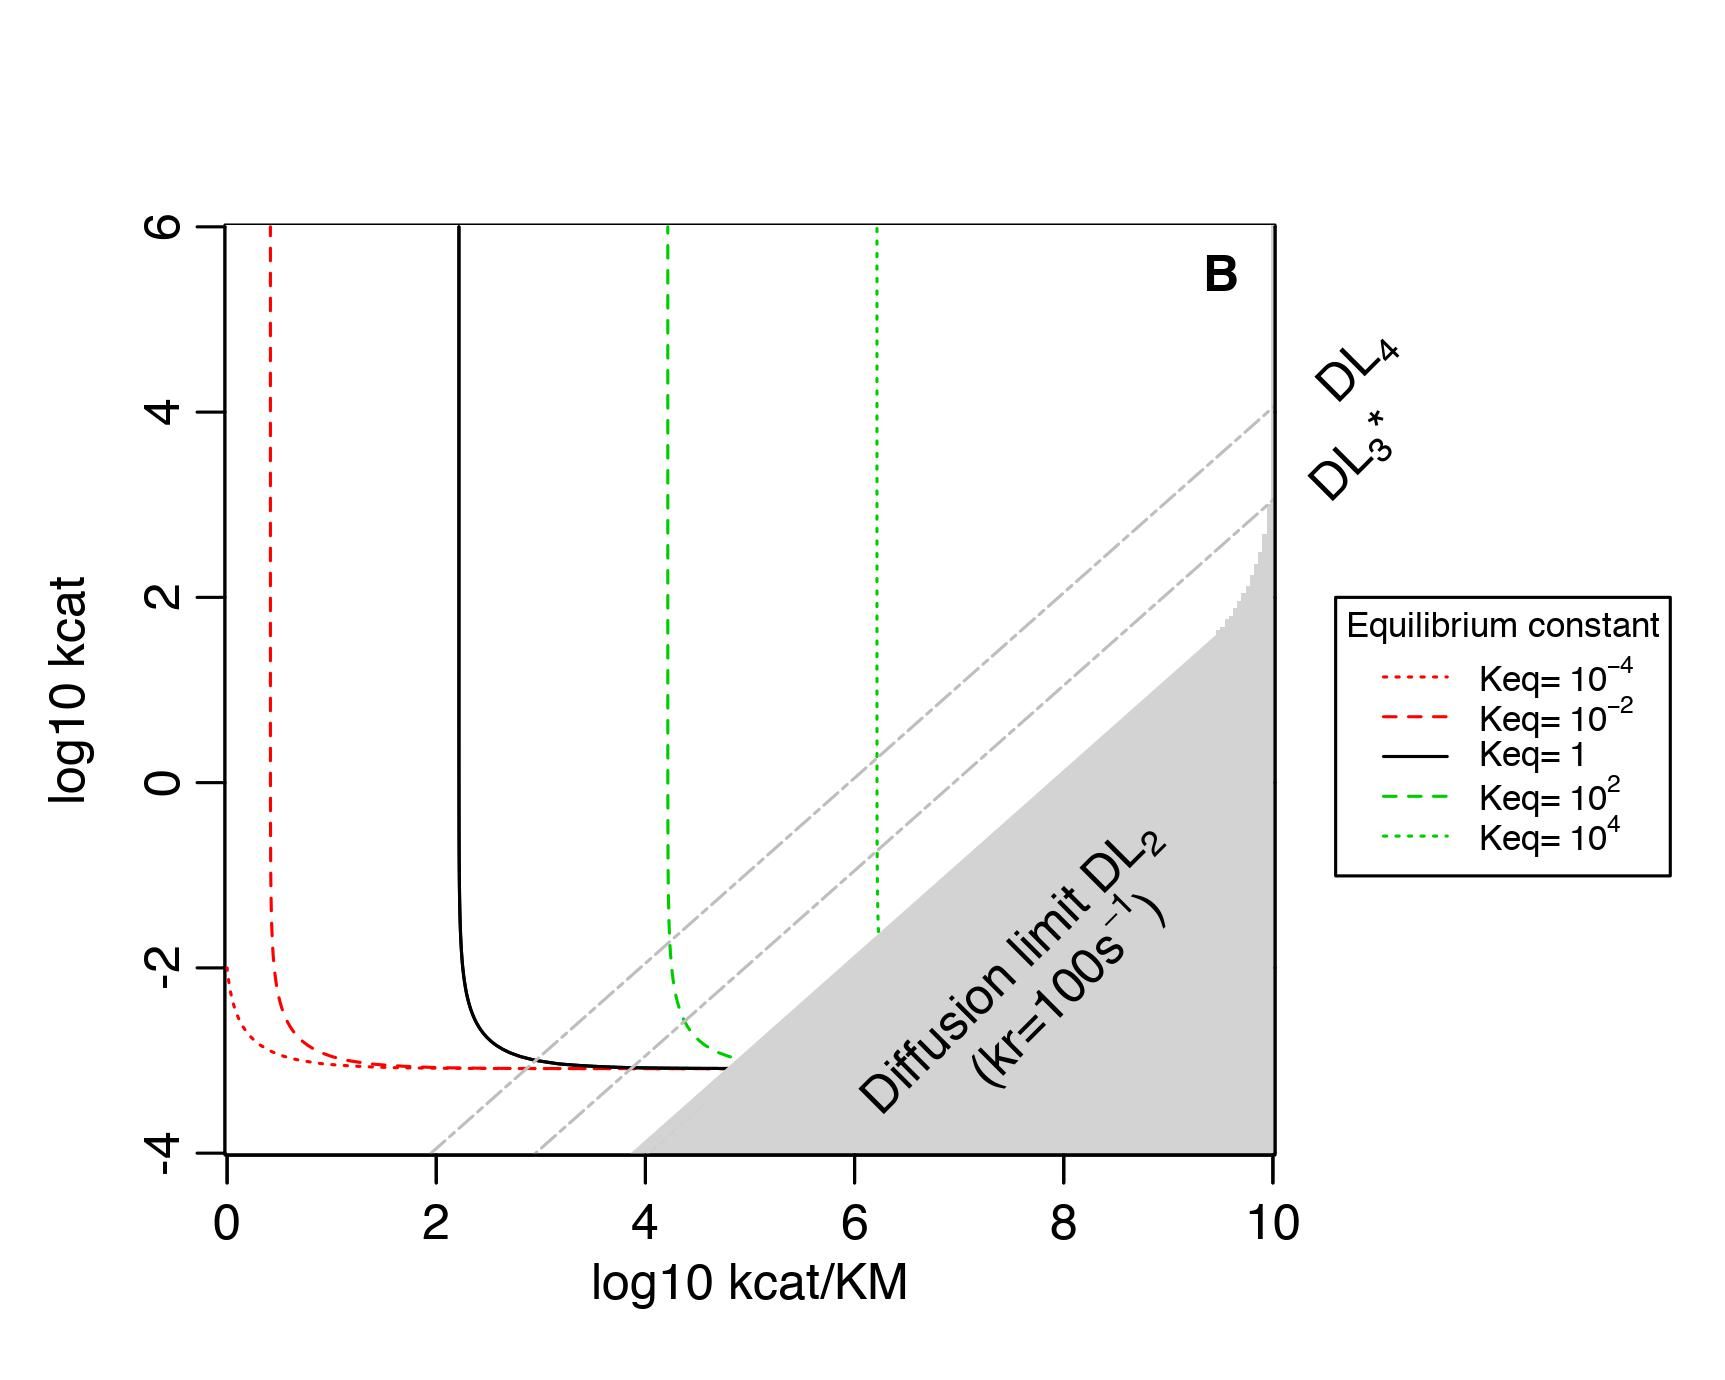
\includegraphics[scale=0.64,trim=0cm 0cm 0cm 1.5cm,clip]{Figures/2DFitLandscape_Multiple_Reverse_exp_par.jpeg}
%DIFDELCMD < \end{minipage}
%DIFDELCMD < %%%
%DIFDELCMD < \caption{%
{%DIFAUXCMD
\DIFdelFL{Backwards reaction rates of an enzyme directly upstream have a strong impact on the fitness landscape. Both plots show results of the influence of the reversibility of the first reaction on the fitness landscape of the next enzyme. Parameters are identical as in FIG.~\ref{figure3D2DFit}, corresponding to the model case for amino acids, with $k_r=10^3s^{-1}$. $K_{eq}$ equals $[S]_{eq}/[P]_{eq}=k_rk_{inh}/k_\text{cat}k_f$ \citep{Klipp94} and quantifies the degree of reversibility, a low $K_{eq}$ featuring low reversibility and vice versa. The first enzyme is a nearly perfect forward enzyme with $k_f=10^{8}M^{-1}$ and $k_{cat}=10^4s^{-1}$. 
Reversibility was equally spread between the two backwards parameters (\textit{e.g.} $K_{eq}=10^2$ yields $k_r=10^{1}k_{cat}$ and $k_{inh}=10^{1}k_f$), and a low degradation rate was considered ($\eta_d=10^{-4}s^{-1}$). In (A), results are plotted in the theoretical parameter space ($k_f, \; k_\text{cat}$), showing that any increase in reversibility increases the pressure on enzyme kinetics by the same magnitude -- except when reactions are highly non-reversible (in red)
. In (B), the same results are shown in the experimenter parameter space of the second enzyme, showing that there is an increased pressure on $k_\text{cat}/K_M$ under higher reversibility. 
While the plateau is not moved upwards, indicative of a selection on $k_\text{cat}$ independent on reversibility when $k_\text{cat}/K_M$ is fixed, positive selection for this parameter may still arise due to the diffusion limit that precludes the access to the lowest $k_\text{cat}$ at high $k_\text{cat}/K_M$. The diffusion limit should play an important role for enzymes with a high dissociation rate $k_r$, as illustrated by the delineation of the diffusion limit (grey area or grey dashed lines) corresponding to several $k_r$ values (eg. DL$_3$ stands for $k_r=10^3s^{-1}$; the star indicates that it is the case represented in (A)).}}
%DIFAUXCMD
%DIFDELCMD < \label{figure2D_Reverse}
%DIFDELCMD < \end{figure*}
%DIFDELCMD < 

%DIFDELCMD < %%%
\DIFdel{Without any }\DIFdelend \DIFaddbegin \DIFadd{In the absence of }\DIFaddend mutational bias ($b=0$), simulated enzymes spread \DIFdelbegin \DIFdel{all }\DIFdelend over the fitness plateau, as expected (\DIFdelbegin \DIFdel{FIG.~\ref{figure2D_Evolutionary_results}A }\DIFdelend \DIFaddbegin \DIFadd{Fig.~S16-A }\DIFaddend for low flux, \DIFdelbegin \DIFdel{Figure S7A of SM }\DIFdelend \DIFaddbegin \DIFadd{Fig.~S17A }\DIFaddend otherwise). The onset of the plateau depends on the strength of drift and hence derive from the effective population size $N_e$, following the classical expectation that selection becomes inefficient when $N_e \times s < 1$ \DIFdelbegin \DIFdel{\citep{Kimura68}}\DIFdelend \DIFaddbegin \DIFadd{\citep{Wright31,Kimura68}}\DIFaddend . Introducing a mutational bias that makes enzyme kinetics less efficient on average has a strong effect on both $k_\text{cat}$ and $k_f$, preventing simulated enzymes from improving far above the drift barrier (FIG.~\ref{figure2D_Evolutionary_results}\DIFdelbegin \DIFdel{B }\DIFdelend \DIFaddbegin \DIFadd{-A }\DIFaddend for low flux, \DIFdelbegin \DIFdel{Figure S7B of SM }\DIFdelend \DIFaddbegin \DIFadd{FIG.~\ref{figure2D_Evolutionary_results}-B }\DIFaddend otherwise). 
Even weak biases (\DIFdelbegin \DIFdel{$b=0.1$}\DIFdelend \DIFaddbegin \DIFadd{$b=-0.1$}\DIFaddend ) lead to enzymes evolving in the vicinity of the isocline where $N_e \times s \approx 1$. Increasing the strength of this bias to $0.2$ only slightly decreases the population variance around this expectation. \DIFaddbegin \DIFadd{Finally, mutational correlations do not impact much the distribution of evolutionary outcomes (SM Fig. S18).
}\DIFaddend 

\DIFdelbegin \DIFdel{In light of this }\DIFdelend \DIFaddbegin \DIFadd{Our results suggest a strong }\DIFaddend effect of the effective population size on enzyme evolution, \DIFdelbegin \DIFdel{the seeming adequation between the plateau and the data in FIG.~\ref{figure2D_BarEven_Dataset} appears puzzling, as the lowest }\DIFdelend \DIFaddbegin \DIFadd{such that species with }\DIFaddend $N_e$ \DIFdelbegin \DIFdel{considered here do not encompass those traditionally found for unicellular organisms that mostly exceed }\DIFdelend \DIFaddbegin \DIFadd{above }\DIFaddend $10^5$ \DIFdelbegin \DIFdel{\citep{Bobay18}. In the same vein, }\DIFdelend \DIFaddbegin \DIFadd{\citep[most unicellular organisms]{Bobay18} should express extremely efficient enzymes. This appears to not be the case, as for instance }\DIFaddend Eukaryotes and Prokaryotes \DIFdelbegin \DIFdel{datasets display similar ranges }\DIFdelend \DIFaddbegin \DIFadd{display similar enzymes }\DIFaddend despite large differences in effective population sizes \citep{Bar-Even11}. \DIFdelbegin \DIFdel{It is thus possible that the role of genetic drift is not well captured by a model that considers small parts of a large system in isolation, or more generally that the link between fitness and flux is not as straightforward as we have assumed}\DIFdelend \DIFaddbegin \DIFadd{As we will later discuss, this conundrum might resolve when considering the smaller size of organisms forming large populations, making them more sensitive to noise in gene expression and favouring higher concentrations}\DIFaddend . 
Notwithstanding this issue, the prediction of enzymes evolving a predictable set of \DIFdelbegin \DIFdel{kinetics parameters when mutational biases are considered contrasts with the broad variability reported \citep{Davidi18}, thereupon requiring further investigation.
}%DIFDELCMD < 

%DIFDELCMD < %%%
\subsection{\DIFdel{Explaining the variance within a pathway}}
%DIFAUXCMD
\addtocounter{subsection}{-1}%DIFAUXCMD
%DIFDELCMD < 

%DIFDELCMD < %%%
\DIFdel{So far, our model predicts that enzymes intervening in a given pathway should evolve on a common fitness landscape, provided that the accumulation of intermediate metabolites is highly detrimental. This should produce similar enzymes along a pathway, which is directly contradicted by empirical estimates, suggesting that each enzyme instead evolves on its own fitness landscape. In this section we show that (1) physical constraints, among which in first place is the reversibility of reactions and (2) the joint evolution of kinetic parameters and other evolving parameters, can explain large differences among enzyme kinetic parameters by influencing actual \textit{in vivo} efficiencies. %DIF < evolvable=susceptible to adapt by NS, peut-être qu'on veut être plus général, mutable?
}%DIFDELCMD < 

%DIFDELCMD < %%%
\DIFdel{Reversibility is an intrinsic feature of chemical reactions that cannot be directly overcome by Evolution \citep{Haldane30,Cornish-Bowden79a}. A highly reversible reaction corresponds to a large intrinsic equilibrium constant $K_{eq}=[S]_{eq}/[P]_{eq}$ \citep{Klipp94}, and results in higher backward than forward rates in the following chemical equation: }\begin{displaymath}
\ce{ E + S <=>[k_{f}][k_{r}] ES <=>[k_{cat}][k_{inh}] E + P_1 }\DIFdel{,
\label{chemMM_fullrev}
}\end{displaymath}%DIFAUXCMD
\DIFdel{where $k_{inh}$ represents the rate at which enzyme and product combine back. Such a (reversible) reaction could in principle influence the selective pressure acting on the following enzyme in the pathway, for both enzymes compete to process the same metabolite $P_1$. We thus quantified how reversibility affects the evolution of an enzyme downstream (FIG.~\ref{figure2D_Reverse} ; using the same model case parameters used throughout the paper (see FIG.~\ref{figure3D2DFit}
for details) and considering a nearly perfect first enzyme for consistency: $k_{cat}=10^4s^{-1}$,$k_f=10^8M^{-1}s^{-1}$).
}%DIFDELCMD < 

%DIFDELCMD < %%%
\DIFdel{The equilibrium constant $K_{eq}$ has a similar (non-linear) impact on the fitness landscape of the second enzyme than the degradation rate, with a highly reversible upstream enzyme exerting a selection pressure downstream towards an increase of kinetic parameters (FIG.~\ref{figure2D_Reverse}-A). Indeed, increasing $K_{eq}$ moves }\DIFdelend \DIFaddbegin \DIFadd{kinetic parameters strongly suggests that a large part of }\DIFaddend the \DIFaddbegin \DIFadd{broad variance in enzyme features is due to differences in the selective context experienced by each, thereupon requiring further investigation on the dependency of the position of the }\DIFaddend fitness plateau \DIFdelbegin \DIFdel{toward the upper-right corner in the ($k_f$,$k_\text{cat}$) parameter space, hence selecting for more efficient downstream enzymes. The effect appears linear, except for very low values of $K_{eq}$ where it fades -- such that a 100-fold change in $K_{eq}$ has little impact -- because the main issue when reactions are highly non-reversible becomes, again, metabolite accumulation. Therefore, the reversibility of the upstream reaction appears like a critical parameter for the evolution of an enzyme, able to generate large changes in evolutionarily expected kinetic parameters . When using the ``empirical" parameter space (FIG.~\ref{figure2D_Reverse}-B), we observe that increasing reversibility only selects for higher $k_\text{cat}/K_M$. Interestingly, the unbinding rate $k_r$ of an enzyme, which is correlated to its reversibility, may eventually favour a positive codependency between the forward rates $k_\text{cat}$ and $k_f$ as the latter is no longer sufficient to ensure a high $k_\text{cat}/K_M$ (see FIG.
~\ref{figure2D_Reverse}-B and Figure S9 of SM for this influence in the theoretical parameter space).
}\DIFdelend \DIFaddbegin \DIFadd{to parameters of our model.
}\DIFaddend 

\DIFdelbegin %DIFDELCMD < \begin{figure}[t!]
%DIFDELCMD < %%%
\DIFdelendFL \DIFaddbeginFL \subsection{\DIFaddFL{The joint evolution of enzyme concentrations and kinetic parameters}}

\begin{figure}[h!]
\DIFaddendFL \centering
\DIFdelbeginFL %DIFDELCMD < \includegraphics[scale=0.58,trim=0cm 0cm 0cm 1.5cm,clip]{Figures/Plot2DFitLandscape_Enz_conc.jpeg} 
%DIFDELCMD < \vspace{-0.3cm}
%DIFDELCMD < %%%
\DIFdelendFL \DIFaddbeginFL 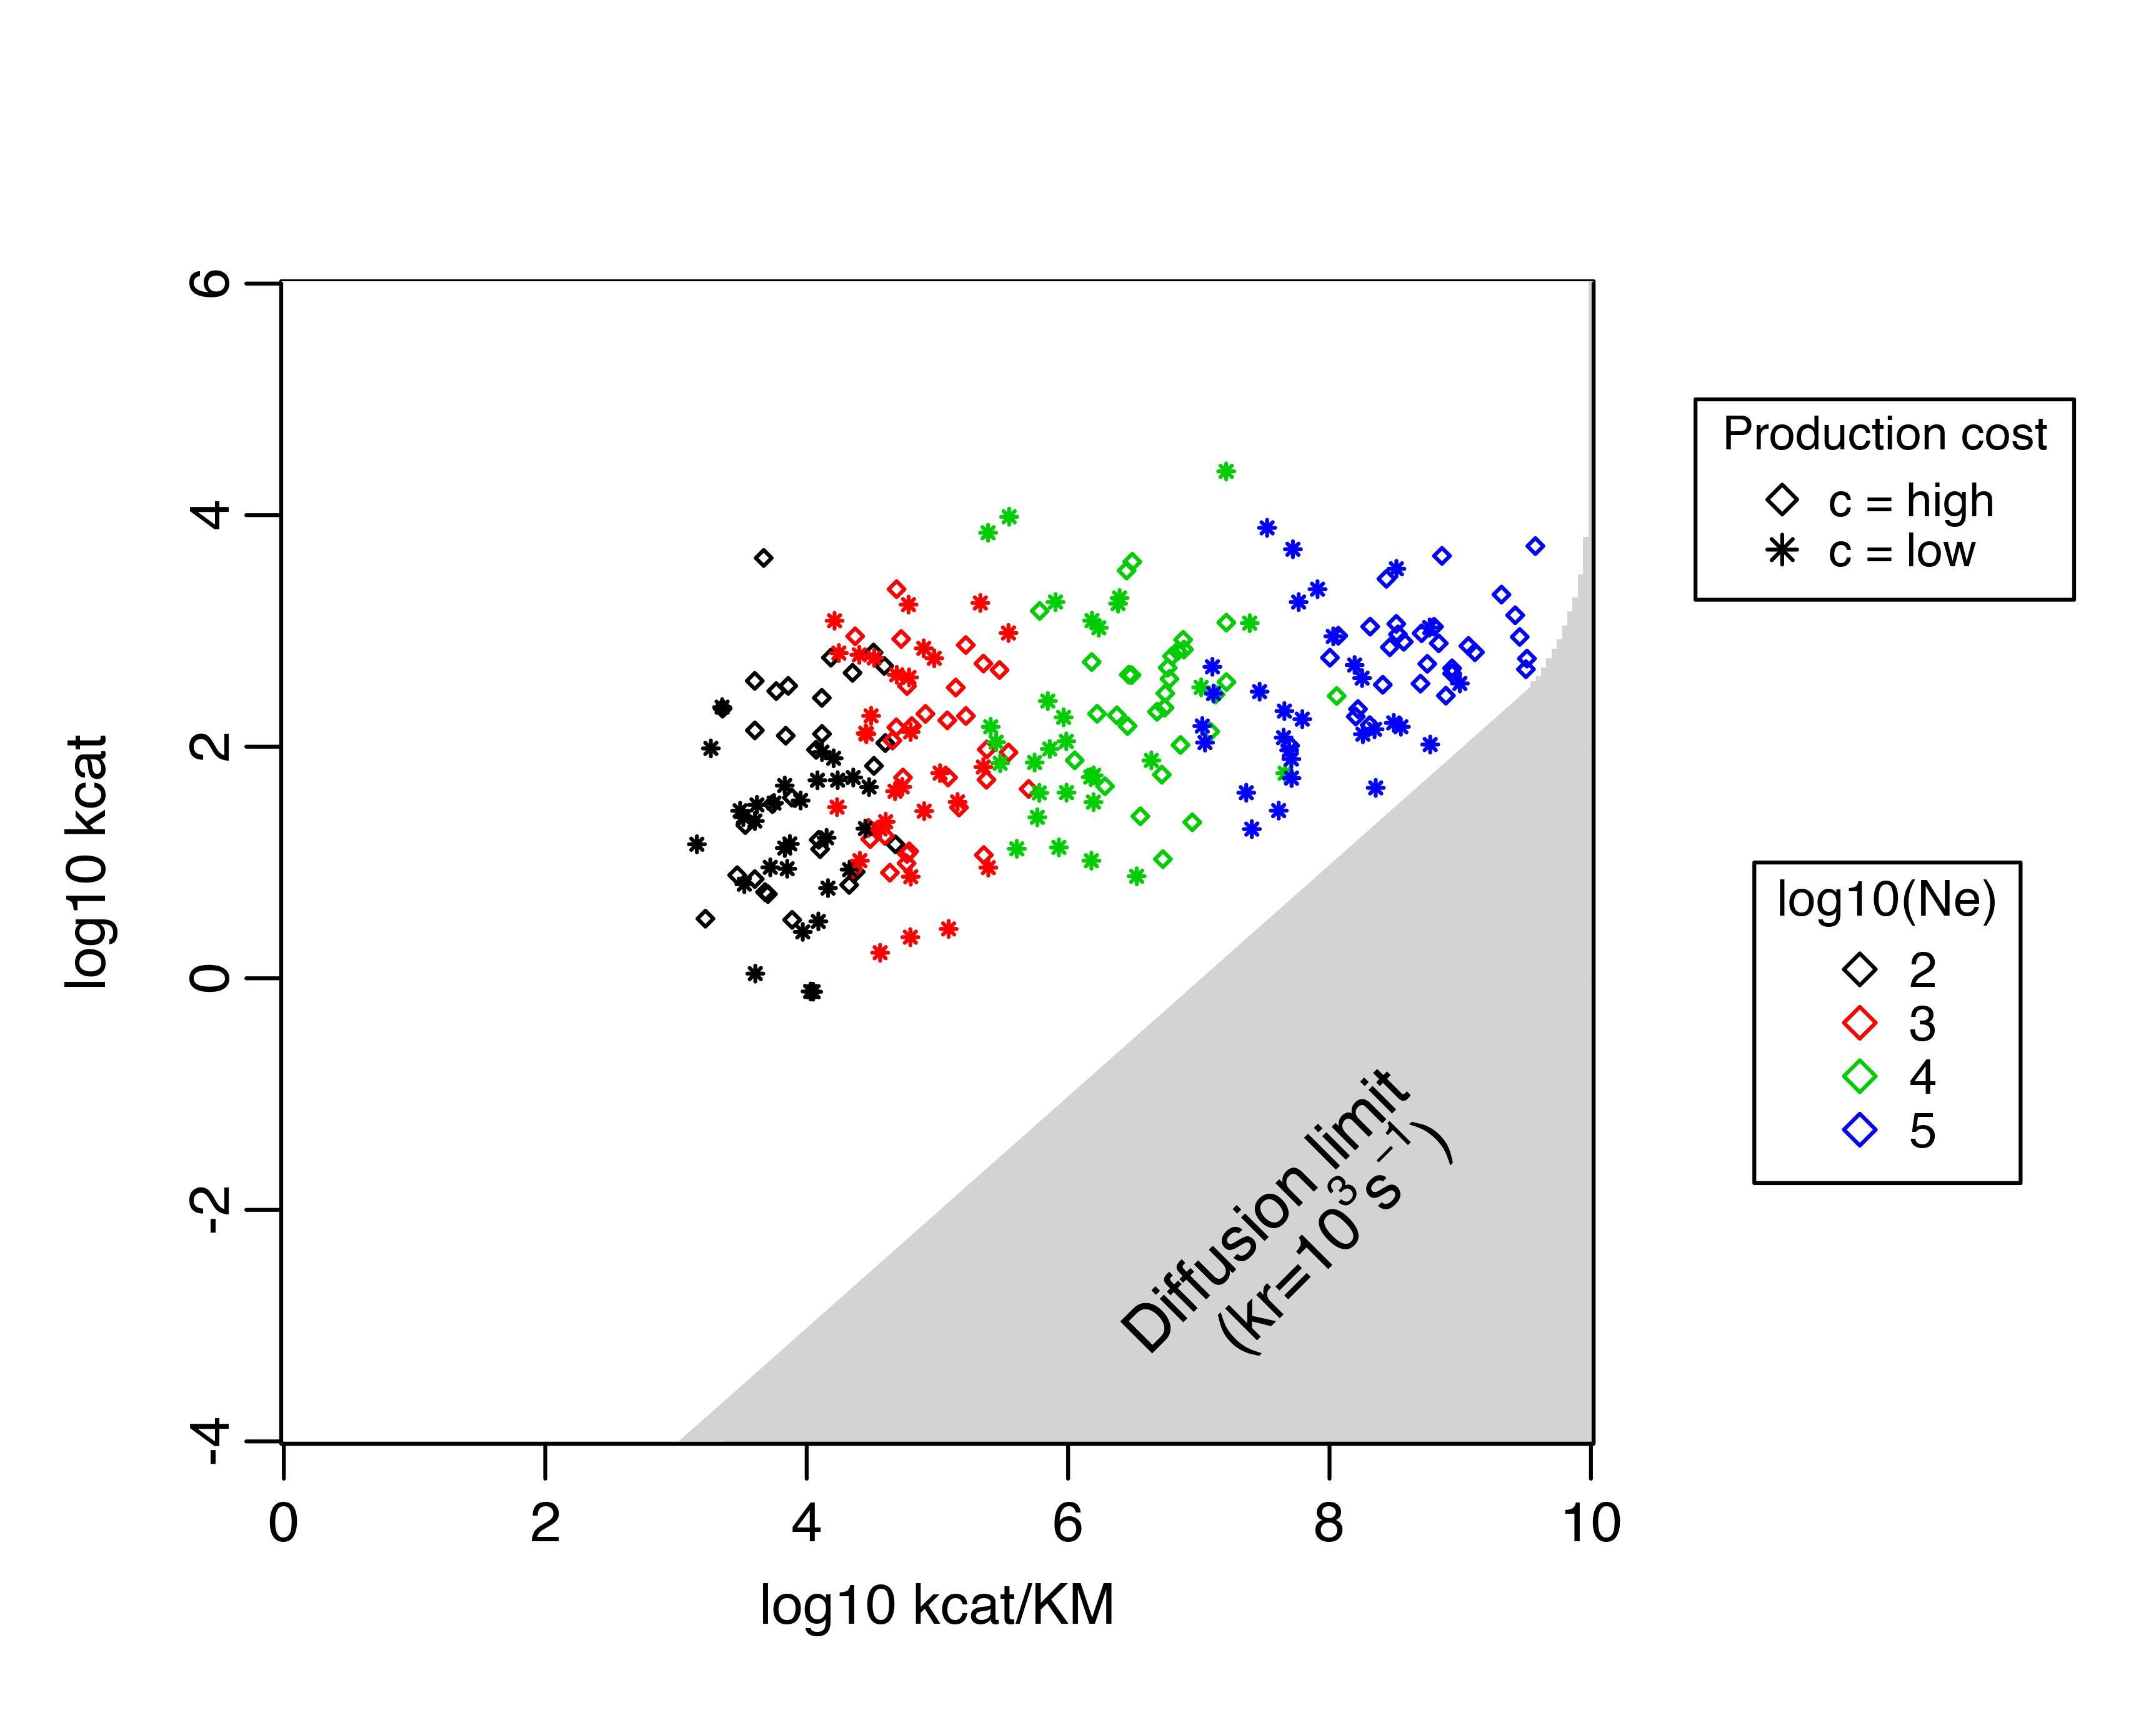
\includegraphics[scale=0.62,trim=0.25cm 0cm 0cm 1cm,clip]{Figures/Evo_Results_CostCrow_PaperModM.jpeg}
\DIFaddendFL \caption{\DIFdelbeginFL \DIFdelFL{High }\DIFdelendFL \DIFaddbeginFL \DIFaddFL{Simulations of the joint evolution of }\DIFaddendFL enzyme concentration \DIFdelbeginFL \DIFdelFL{$[E_{tot}]$ alleviate selection on both $k_\text{cat}/K_M$ }\DIFdelendFL and \DIFdelbeginFL \DIFdelFL{$k_\text{cat}$}\DIFdelendFL \DIFaddbeginFL \DIFaddFL{kinetic parameters, with a twofold cost of enzyme overexpression (the direct metabolic cost and the indirect cost of cell packing)}\DIFaddendFL . The \DIFdelbeginFL \DIFdelFL{parameters for transport }\DIFdelendFL \DIFaddbeginFL \DIFaddFL{case considered here is that of a transporter with a high flux at saturation and low affinity ($V_{Tm}=1 mMs^{-1}$ and $K_T=1mM$) under a high mutational bias on kinetic constants ($b=-0.2$). Two different costs of protein production $c$ }\DIFaddendFL are \DIFaddbeginFL \DIFaddFL{considered along with four effective population sizes ranging from $10^2$ to $10^5$. We ran 30 independent simulations for each scenario, each represented by a dot in }\DIFaddendFL the \DIFdelbeginFL \DIFdelFL{same than }\DIFdelendFL \DIFaddbeginFL \DIFaddFL{``empirical" parameter space as described }\DIFaddendFL in \DIFdelbeginFL \DIFdelFL{FIG}\DIFdelendFL \DIFaddbeginFL \DIFaddFL{fig}\DIFaddendFL .~\DIFdelbeginFL \DIFdelFL{\ref{figure3D2DFit}, with $k_r=10^3s^{-1}$}\DIFdelendFL \DIFaddbeginFL \DIFaddFL{\ref{figure2D_Evolutionary_results}}\DIFaddendFL .
}
\DIFdelbeginFL %DIFDELCMD < \label{figure2DEnzconc}
%DIFDELCMD < %%%
\DIFdelendFL \DIFaddbeginFL \label{figure2D_Evolutionary_results_HF}
\DIFaddendFL \end{figure}

Hitherto, we have considered enzymes to be highly concentrated, an assumption that we \DIFdelbegin \DIFdel{relax here}\DIFdelend \DIFaddbegin \DIFadd{now relax since it is an important component of the presumed kinetic activity \citep{Koshland02}}\DIFaddend . Predictably, increasing the concentration of the first or second enzyme in a pathway releases the selection on their kinetic parameters \citep{Noor16}, producing larger fitness plateaus as an enzyme concentration increases (see \DIFdelbegin \DIFdel{FIG.~\ref{figure2DEnzconc} for the first enzyme and Figure S10 of SM for the second). Because the concentration is subject to heritable changes \citep{Schaefke13}}\DIFdelend \DIFaddbegin \DIFadd{SM - Figs S12-B and S13-B for this influence in different contexts). Due to the compensatory effects between concentration and activity}\DIFaddend , we anticipate that the joint evolutionary dynamics of the concentration and kinetic parameters should yield a negative correlation between them, as reported by \citet{Davidi16,Davidi18}\DIFdelbegin \DIFdel{(who focused on $k_\text{cat}[E]_{tot}$) , due to the compensatory effect of concentration}\DIFdelend . 

\DIFaddbegin \DIFadd{Despite their common role on reaction efficiency, enzyme concentration expectedly responds to very different selection pressures than kinetic parameters, as increased gene expression levels come with costs \citep{Wagner05,Lang09,ScottM10,Noor16,Kafri16}. Indeed, producing extra proteins requires both energy and matter \citep{Novick57,Stoebel08,Wagner05,Lynch15} and may impede the efficiency of physical processes that rely on an optimal intermediate content \citep{Dong95,Dill11,Andrews20}. We designed a new instance of our population genetics model to study the tangled evolution of kinetic constants and enzyme concentration, introducing two of these costs: (1) the cost of producing proteins $c$, considered to be proportional to concentration \citep{Wagner05,Chou14,Lynch15}, and (2) the exponential cost of an increase in macromolecular crowding, which hinders diffusion and thus slows down reactions \citep{Dill11,Schavemaker18,Andrews20} 
%DIF >  when cellular concentrations go beyond a threshold $[Proteome] \approx 3-4 mM$ 
(see SM Fig. S15 for the resulting fitness landscapes of enzyme concentration).
}

\DIFadd{The two types of costs result in a different shape of the fitness landscape, with the noticeable difference that evolutionarily expected concentration depends on $N_e$ when the cost of production is considered (SM - Fig. S19) but not with crowding effects (SM - Fig. S20). With a combination of the two costs, enzyme concentrations decrease with $N_e$ and production costs, resulting in the evolution of higher kinetic constants (FIG. \ref{figure2D_Evolutionary_results_HF}). This is because at higher effective sizes, direct costs of protein production are large enough to incur effective selection for lower protein expression. This is no longer the case when $N_e$ decreases, such that the major force driving the optimization of enzyme concentration becomes that opposing macromolecular crowding, which is less sensitive to $N_e$ (as shown in Fig. S19 in SM). The balance between these two selective forces, and the dependency to $N_e$, obviously depend on the relative importance of these costs (SM - Fig. S20), itself depending on many parameters (protein length, molecular weight, etc.) that should only make enzymes marginally different within a given species (when their activity evolves on similar fitness landscapes).
}

\DIFaddend \section{Discussion\label{sec:Discussion}}

Most enzymes have been considered to be only moderately efficient \DIFaddbegin \DIFadd{\citep{Bar-Even11}}\DIFaddend , if not sloppy \DIFdelbegin \DIFdel{\citep{Bar-Even11,Bar-Even15}}\DIFdelend \DIFaddbegin \DIFadd{\citep{Bar-Even15}}\DIFaddend . This claim was put into perspective by \citet{Newton18} who argued that the link between fitness and enzyme efficiencies is complex and may be partly \DIFdelbegin \DIFdel{enzyme-dependent}\DIFdelend \DIFaddbegin \DIFadd{enzyme dependent, such that all enzymes may not evolve on a common fitness landscape}\DIFaddend . Through this work, we have developed a model where enzyme efficiencies are mechanistically linked to fitness through the impact of nutrient gradients on the production of metabolites. Our results emphasize that \DIFdelbegin \DIFdel{enzymes might in fact be quite efficient and , possibly, as efficient as Evolution allows. 
}%DIFDELCMD < 

%DIFDELCMD < %%%
\DIFdel{We have modelled two processes of nutrient uptake that rely heavily on concentration gradients: passive (PD) and facilitated diffusion (FD). Our results apply to the numerous metabolic pathways that start with them, and also possibly to the widely used secondary active transport (SAT) in which FD of ion-substrate complexes follows the active extraction of a cotransported ion.
Indeed, SAT can be described by similar equations as FD, with the difference that energy is required for extraction \citep{Stein86e}.
}%DIFDELCMD < 

%DIFDELCMD < %%%
\DIFdel{Our results indicate that an enzyme's forward kinetic parameters }\DIFdelend \DIFaddbegin \DIFadd{an enzyme's fitness landscape -- and the resulting mutation-selection-drift balance }\DIFaddend -- \DIFdelbegin \DIFdel{$k_\text{cat}$ and $k_f$ -- evolve on cliff-like fitness landscapes with a plateau -- where the flux of energy generated increases on a log scale -- }\DIFdelend \DIFaddbegin \DIFadd{may indeed be largely context dependent, possibly explaining a large part of the extreme observed variance in enzyme features.
}

\DIFadd{At first sight, all enzymes evolve on fitness landscapes that have the same general shape, with a fitness plateau }\DIFaddend surrounded by a steep slope. \DIFdelbegin \DIFdel{This conclusion seems to agree qualitatively with the assumptions of previous models \citep{Hartl85,Kaltenbach14}, which we confirm here from a nutrient driven perspective.
Importantly, our framework allows to consider the joint evolution of two kinetic parameters, $k_f$ and }\DIFdelend \DIFaddbegin \DIFadd{While this shape is usual in models of enzyme evolution \citep{Hartl85,Kaltenbach14,Yi19}, in our model the landscape is drawn in the parameter space formed by the two forward kinetic parameters }\DIFaddend $k_\text{cat}$ \DIFaddbegin \DIFadd{and $k_f$, }\DIFaddend instead of a composite ``efficiency\DIFdelbegin \DIFdel{" }\DIFdelend \DIFaddbegin \DIFadd{'' }\DIFaddend whose relevance is questionable \DIFdelbegin \DIFdel{\citep{Koshland02,Eisenthal07}, and to pinpoint model parameters that have a differential impact on each. This, along with our broad comparison of model predictions with a massive dataset, initiates an attempt to predict evolutionary trends at the level of individual enzymes. 
We show that this should be possible in principle, under the assumption that mutations of efficient enzymes are slightly biased towards making them less efficient, which limits evolutionary predictions to a narrow range in the parameter space.
}%DIFDELCMD < 

%DIFDELCMD < %%%
\DIFdel{Overall, }\DIFdelend \DIFaddbegin \DIFadd{\citep{Eisenthal07,Koshland02}. Our model allows to predict the precise position of the fitness plateau in various contexts, showing that model parameters may have a selective impact on $k_f$, $k_\text{cat}$, or both, thereby confirming the relevance of considering their distinct evolutionary dynamics. 
}

\DIFadd{We have shown that }\DIFaddend the \DIFaddbegin \DIFadd{exact position of the plateau is important through a population genetics model including mutational biases that produce less efficient enzymes at a slightly higher frequency. Despite their small effect, these biases are sufficient to have a significant impact on the evolutionary dynamics occurring on the fitness plateau, preventing enzymes to explore the parameter space far away from an isocline whose precise value can be predicted. Because the mutation-selection-drift balance occupies a narrow part of the landscape, this makes the }\DIFaddend evolution of an enzyme\DIFdelbegin \DIFdel{should result }\DIFdelend \DIFaddbegin \DIFadd{, in principle, highly predictable. Likewise, we anticipate that differences between enzymes should largely be explained by differences in the shapes of their individual fitness landscapes. 
}

\DIFadd{Overall, the selective pressure acting on an enzyme results }\DIFaddend from an interplay between \DIFdelbegin \DIFdel{(1) ecological and biochemical factors-- metabolic demands, richness of the environment, reversibility of reactions -- that draw the landscape, and (2) evolutionary factors -- effective population size, distribution of mutational effects -- governing how organisms move through evolutionary times on these landscapes}\DIFdelend \DIFaddbegin \DIFadd{several biochemical factors}\DIFaddend . We have effectively found that the shape of the fitness landscape \DIFdelbegin \DIFdel{depends on }\DIFdelend \DIFaddbegin \DIFadd{is first governed by }\DIFaddend features of the transporter \DIFdelbegin \DIFdel{, namely }\DIFdelend \DIFaddbegin \DIFadd{initiating a pathway, especially }\DIFaddend the maximum flux they can sustain\DIFdelbegin \DIFdel{and their affinity for the substrate, each having different effects on $k_\text{cat}$ and $k_f$. These features are themselves evolving quantities, and the joint evolution of transporters and intracellular enzymes remains to be studied. Yet, using }\DIFdelend \DIFaddbegin \DIFadd{. Using }\DIFaddend parameters that correspond to empirical estimates for sugars and amino acids\DIFaddbegin \DIFadd{/nucleosides}\DIFaddend , we have found that enzymes \DIFdelbegin \DIFdel{intervening in }\DIFdelend \DIFaddbegin \DIFadd{contributing to }\DIFaddend subsequent metabolic pathways should be different, with those in the ``sugars" pathway being selected for faster kinetics.
\DIFdelbegin \DIFdel{The focus in this study was not on interactions within a pathway and high-order epistasis, but our framework suggests that all enzymes but the first in a pathway should evolve on fitness landscapes that do not depend on their position, as long as all upstream enzymes belong to the fitness plateau. If one enzyme is noticeably inefficient, however, selection will push downstream enzymes towards a wider plateau, as a larger region of the parameter space can accommodate such a lower flux.
}\DIFdelend 

\DIFdelbegin \DIFdel{We also notice that different constraints may be met along a pathway and make each enzyme }\DIFdelend \DIFaddbegin \DIFadd{While sharing a common transporter, enzymes along a pathway are also subject to a variety of local chemical contexts, making each }\DIFaddend evolve on its own \DIFdelbegin \DIFdel{fitness landscape, possibly explaining a partof the large variance reported at this scale}\DIFdelend \DIFaddbegin \DIFadd{unique fitness landscape. This could explain, at least in part, the large within-pathway variance of enzyme kinetic parameters}\DIFaddend . Physical constraints may for instance act differentially on different enzymes, as exemplified by the intrinsic reversibility of a reaction that fuels the selective pressure towards higher efficiency in downstream enzymes. This may contribute to explain the high efficiency of a few \DIFdelbegin \DIFdel{specific enzymes , and thereby why there exists some ``equilibrium enzymes" pushing reactions close to equilibrium \citep{Williamson67,Davidi18}. Aside from physical constraints, actual enzyme kinetic parameters are entangled with many more biochemical parameters, making the prediction of their evolution complex. 
}\DIFdelend \DIFaddbegin \DIFadd{enzymes like TIM %DIF > , and thereby why there exists some ``equilibrium enzymes" pushing reactions close to their chemical equilibrium 
\citep{Williamson67,Davidi18}.
}\DIFaddend 

\DIFdelbegin \DIFdel{More specifically, we have examined the effect of one such parameter (but not its evolution), the concentration of the enzyme}\DIFdelend \DIFaddbegin \DIFadd{One way to compensate for low kinetic constants is to enhance the level of expression of an enzyme, as confirmed by our model -- concentration indeed has a strong influence on the fitness landscape of $k_f$ and $k_\text{cat}$. Nonetheless, concentration and kinetic parameters face very distinct selection regimes: while the latter are both under directional selection, vanishing at high efficiencies, concentration is under stabilizing selection -- owing to a combination between its positive impact on the flux and the adverse costs to high expression -- as already pinpointed by \citet{Chou14}. Their joint evolution is complex because the position of the concentration optimum depends on an enzyme's kinetic constants, whose fitness landscape itself depends on concentration. This results in a slightly increased variance in enzyme efficiencies compared to simulations with fixed concentrations, along with a complex relationship with genetic drift, because small populations tend to tolerate higher enzyme concentrations and, therefore, evolve less efficient enzymes.
}

\DIFadd{It should be noted that our model does not consider another selection pressure on enzyme concentrations that arises from noise in gene expression}\DIFaddend , \DIFdelbegin \DIFdel{showing that it indeed exerts an important role and is likely involved in the variance in $k_f$ and $k_\text{cat}$, for low efficiency can be buffered by high levels of expression andvice versa.
How enzyme levels of expressionand efficiencies jointly evolve, including the role of the cellular content on these efficiencies, should be the next step forward in the understanding of enzyme evolution. Because a cell is packed with many organites and biomolecules, making diffusion less efficient and $k_f$s lower \textit{in vivo} than their \textit{in vitro} counterparts, opposing forces govern the evolution of enzyme concentrations. Increasing concentrations may thus come at a great cost by slightly but steadily decreasing the actual efficiency of many catalysts at once, in turn favouring the evolution of highly efficient enzymesunless physical constraints prevent such an improvement. }\DIFdelend \DIFaddbegin \DIFadd{as argued by \citet{Wang11}. Indeed, low expression results in detrimental noise that should be avoided by pushing enzyme concentrations towards higher values in small organisms like Prokaryotes (see SM section Text S6 for an estimate of this effect). This could result in a different relationship between $N_e$ and enzyme efficiencies than considered here, possibly explaining the confusing observation that species with larger populations (and smaller sizes) do not express markedly more efficient catalysts. Furthermore, an enzyme's effective concentration can also increase through compartmentalization \citep{Ovadi04,Diekmann13,Cornejo14} and substrate channeling \citep{Welch94,Huang01,Sweetlove18}, within the limits imposed by noise, and modify the selective pressure acting on kinetic parameters.
}\DIFaddend 

\DIFdelbegin \DIFdel{Our work provides a mechanistic model for enzyme evolution, based on the assumption that }\DIFdelend \DIFaddbegin \DIFadd{This illustrates that rather than making precise predictions, our study aims at making the strong claim that selection acting on enzyme features is important for their diversity, possibly largely overcoming the diversity arising from neutral processes. If this is indeed the case, trends in enzyme evolution can be predicted -- as it was shown empirically in the context of antibiotic resistance \citep{Walkiewicz12} -- and further improvements of this model should allow to predict the expected features of individual enzymes. Such improvements are made easier by the use of a mechanistic framework, where fitness arises as }\DIFaddend enzymatic efficiency helps ingesting nutrients and win the competition for resources. \DIFaddbegin \DIFadd{This framework could even be enriched by other dimensions relevant to the genotype-phenotype-fitness map \citep{Bershtein17,Echave19,Kinsler20}. 
}

\DIFaddend Unfortunately, mechanistic does not mean free of a definition of fitness, as we have \DIFaddbegin \DIFadd{here }\DIFaddend assumed that the latter is proportional to metabolic flux, hence considering each flux in isolation. Fitness instead results from a wide range of metabolic pathways that combine together and should all be competitive to certain degrees. How \DIFdelbegin \DIFdel{high-order }\DIFdelend \DIFaddbegin \DIFadd{global }\DIFaddend epistasis builds up \DIFaddbegin \DIFadd{\citep{Weinreich13,Otwinowski18,Reddy20}}\DIFaddend , and genetic drift acts in this context, is far from obvious \DIFdelbegin \DIFdel{; but }\DIFdelend \DIFaddbegin \DIFadd{\citep{Iwasa04,Weinreich05,Weissman09}. But }\DIFaddend this should not impact much how enzymes evolve in old, overall efficient pathways, as any impediment in efficiency should have \DIFdelbegin \DIFdel{an }\DIFdelend \DIFaddbegin \DIFadd{a relatively }\DIFaddend independent effect on fitness in this context, as captured by our model. \DIFdelbegin \DIFdel{Yet, this could make selection weaker in some or all pathways , as exemplified by \citet{Heckmann18}, and therefore help explain why they appear to be evolutionary suboptimal. But more importantly, such a model would }\DIFdelend \DIFaddbegin \DIFadd{Understanding these complex interactions between pathways would nevertheless }\DIFaddend be crucial to understand how metabolic pathways arose and improved, likely from a highly inefficient state during early steps in the evolution of life on Earth \DIFaddbegin \DIFadd{\citep{Kacser84,Schmidt03,Heckmann18}}\DIFaddend .

\section{Materials and Methods\label{sec:M&M}}

\subsection{Quantifying the maximum size for cells using passive diffusion}

If a cell is to be viable, it has, at least, to uptake enough glucose to compensate for basal metabolism -- metabolism that allows to maintain the same cell size for non-actively growing cells \citep{Lynch15} -- leading to the following equation: $\phi_{PD}=C_M$, with $\phi_{PD}$ the uptake through passive diffusion and $C_M$ the basal metabolism demand. To calculate the maximum size a cell can reach using only passive diffusion, we relied on the formula $C_M=0.39V^{0.88} (10^9 ATP/hr)$ estimated in \citep{Lynch15}. We also assumed the cell to be of spherical shape, both concentrations -- inside and outside the cell -- to be constant with the cellular concentration staying so low that it can be overlooked, meaning that the uptake resulting from passive diffusion can merely be written as $\phi_{PD}=P.[S_{\text{out}}].\frac{SA_{\text{sphere}}}{V_{\text{sphere}}}$, where $SA_{\text{sphere}}$ and $V_{\text{sphere}}$ are the surface area and the volume of a sphere, and $P$ represents the cell permeability and was measured to $10^{-6}\mu m^{-1}$ \citep{Wood68} for glucose. Finally, we considered that each glucose yields 30 ATP molecules \citep{Rich03}. 

\subsection{Flux sustained by the first enzyme}

When assessing the flux of product made by the first enzyme in a pathway, both (PD) and (FD) result in similar sets of equations; we focus on FD here (see Text S5 - Mathematical appendix in Supplementary material for a comparison with PD). FD typically relies on the specific binding of substrate molecules -- located outside the cell -- by transmembrane carrier proteins, followed by their translocation into the cytoplasm \DIFdelbegin \DIFdel{\citep{danielli1954,Wilbrandt61,Kotyk67}}\DIFdelend \DIFaddbegin \DIFadd{\citep{danielli1954,Wilbrandt61,Kotyk67,Bosdriesz18}}\DIFaddend . This specific process obeys Michaelis Menten-like kinetics when transport is assumed to be symmetric \citep{Kotyk67}, which can be modelled through Briggs-Haldane equations \citep{Briggs25,Haldane30,Stein86d}:
\DIFaddbegin 

\DIFaddend \small
\begin{equation}
\frac{d[S_\text{in}]}{dt}=V_{Tm}.\frac{[S_\text{out}]-[S_\text{in}]}{K_T+([S_\text{out}]+[S_\text{in}])+\alpha.\frac{[S_\text{out}][S_\text{in}]}{K_T}}
\end{equation}
\normalsize

with:
\small
\begin{equation*}
  \left\{
      \begin{aligned}
		&V_{Tm}\text{: the maximum rate of a given carrier protein;}\\
		&K_T\text{: a constant inversely proportional to the transpor-}\\
		&\text{  ter efficiency};\\
		&\alpha \text{ : the Kotyk interactive constant  capturing the dis-}\\
		&\text{  equilibrium between bound and free transporters.}
      \end{aligned}
    \right.
\end{equation*}
\normalsize

%DIF < Alongside the concentration gradient, the Kotyk interactive constant \cite{Kotyk67} also brings by something special because the efflux (\textit{i.e. outwards flow}) cannot be overlooked due to the emergence of saturation in the process \citep{Teusink98,Bosdriesz18}.
By construction, $\alpha$ cannot exceed 1 \cite{Kotyk67} and is close to this upper limit for sugars (\textit{e.g.} $\alpha=0.91$ for glucose \citep{Teusink98}, so we set $\alpha=1$ by default in this study, maximizing the effect of interaction).

A model including both FD and irreversible substrate conversion by an enzyme therefore corresponds to the following chemical equation:

\begin{equation}
\footnotesize
\schemestart
 S$_{out}$
 \arrow{<=>[$V_{Tm},K_T$][$\alpha$]}
 S$_{in}$ + E
 \arrow{<=>[$k_{f}$][$k_{r}$]}
 ES
 \arrow{->[*0$k_{\text{cat}}$]}
 E + P$$
\schemestop
\label{chemMMT1R}
\end{equation}

Using analytical tools (see \citet{Kuile94} \DIFaddbegin \DIFadd{and \citet{Bosdriesz18}}\DIFaddend , rederived in Supplementary material - Text S5 Mathematical appendix), the flux can be determined through the following set of equations:

\vspace{-0.25cm}
\small
\begin{align}
\strut
[ES]^*=\frac{k_f[S_{in}]^*}{k_{r}+k_{cat}+k_f[S_\text{in}]^*}.[E_{tot}]\\
v=\frac{d[P]}{dt}=k_{cat}[ES]^*
\end{align}
\DIFdelbegin %DIFDELCMD < \normalsize
%DIFDELCMD < %%%
\DIFdelend 

\DIFaddbegin \normalsize
\DIFaddend where:
\vspace{-0.25cm}
\DIFaddbegin 

\DIFaddend \small
\begin{align}
[S_\text{in}]^*=\frac{-b+\sqrt{b^2-4ac}}{2a}
\end{align}
\DIFdelbegin %DIFDELCMD < \normalsize
%DIFDELCMD < %%%
\DIFdelend 

\DIFaddbegin \normalsize
\DIFaddend with:
\small
\begin{equation}
  \left\{
      \DIFdelbegin %DIFDELCMD < \begin{aligned}
%DIFDELCMD <         a&=k_f k_{cat}[E_{tot}](1+\frac{[S_{in}]}{K_T})+k_fV_{Tm}\\
%DIFDELCMD < 		b&=k_f k_{cat}[E_{tot}]([S_{in}]+K_T)+(k_{cat}+k_r-k_f[S_{in}])V_{Tm}\\
%DIFDELCMD < 		c&=-V_{Tm}[S_{in}](k_r+k_{cat})\\
%DIFDELCMD <       \end{aligned}%%%
\DIFdelend \DIFaddbegin \begin{aligned}
        a&=k_f k_{cat}[E_{tot}](1+\frac{[S_{out}]}{K_T})+k_fV_{Tm}\\
		b&=k_f k_{cat}[E_{tot}]([S_{out}]+K_T)+(k_{cat}+k_r-k_f[S_{out}])V_{Tm}\\
		c&=-V_{Tm}[S_{out}](k_r+k_{cat})\\
      \end{aligned}\DIFaddend 
    \right.
\end{equation}
\DIFaddbegin 

\DIFaddend \normalsize

%DIF < \vspace{-0.5CM}
%DIF <  Because of the Kotyk interaction constant -- set to $1$ -- the flux cannot reach the value of $V_{Tm}$, and rather stabilizes around an amount of product formed $\frac{d[P]}{dt}=0.9\mu M.s^{-1}$. In SM possibly
\DIFdelbegin %DIFDELCMD < 

%DIFDELCMD < %%%
\DIFdelend \subsection{Multiple enzymes model}

In order to study the evolution of downstream enzymes, we considered an unbranched metabolic pathway in which the product formed by the first reaction serves as the substrate for a second reaction \DIFaddbegin \DIFadd{whose flux determines fitness}\DIFaddend . Theoretically, as there is nothing prohibiting increase in product concentrations -- for it is not considered reversible at this point -- any second enzyme should be able to sustain any metabolic demand. We penalized large increases in cellular concentrations through a degradation process of the product of the first reaction, occurring at rate $\eta_d$ ($\times$ this concentration). 
\DIFdelbegin \DIFdel{Under these new assumptions, the }\DIFdelend \DIFaddbegin \DIFadd{The }\DIFaddend chemical reactions occurring after uptake (Michaelis Menten part of Eq.\ref{chemMMT1R}) are described by the following equations:

\small
\begin{align}
\schemestart
 S$_{in}$ + E$_1$
 \arrow{<=>[$k_{f1}$][$k_{r1}$]}
 E$_1S$
 \arrow{->[*0$k_{\text{cat}1}$]}[0]
 E$_1$ + P$_{1}$
 \schemestop
 \label{chemMMT1R_deg}
 \end{align}
 \begin{align}
 \schemestart
 P$_{1}$ + E$_2$
 \arrow{<=>[$k_{f2}$][$k_{r2}$]}
 E$_2$P$_1$
 \arrow{->[*0$k_{\text{cat2}}$]}[0]
 E$_2$ + P$_{2}$
 \arrow(@c1--){->[*0$\eta_d$]}[-90]
 P$_{1out}$
\schemestop
\label{chemMMT2R_deg}
\end{align}
\DIFdelbegin %DIFDELCMD < \normalsize
%DIFDELCMD < %%%
\DIFdelend 

\DIFaddbegin \normalsize
\DIFaddend Such a system may reach a steady-state at which the cellular concentrations of the substrate $S_{in}$ and of the first product $P_1$ are constant. At this point, the net instantaneous uptake of substrate \DIFdelbegin \DIFdel{(through the membrane) }\DIFdelend equals the instantaneous production of $P_1$ which, in turn, equals the \DIFdelbegin \DIFdel{addition of the instaneous }\DIFdelend \DIFaddbegin \DIFadd{sum of the instantaneous }\DIFaddend amount of degraded $P_1$ and the instantaneous production of $P_2$, according to the principle of mass conservation. It yields the following system of equations:

\footnotesize

\begin{equation}
		\begin{aligned}
V_{Tm}.&\frac{([S_{out}]-[S_{in}])}{K_T+([S_\text{out}]+[S_\text{in}])+\alpha.\frac{[S_\text{out}][S_\text{in}]}{K_T}}=V_{m1}.\frac{[S_{in}]}{K_{M1}+[S_{in}]}
		\end{aligned}
		\label{mathMMT1R_deg}
\end{equation}

\begin{equation}
\begin{aligned}
V_{m1}.&\frac{[S_{in}]}{K_{M1}+[S_{in}]}=V_{m2}.\frac{[P_1]}{K_{M2}+[P_1]}+\eta_d.[P_1]
		\end{aligned}
		\label{mathMMT2R_deg}
\end{equation}
\DIFaddbegin 

\DIFaddend \normalsize
\noindent where appear the traditional Michaelis-Menten kinetic parameters for the (i$^{eth}$) reaction:
\DIFaddbegin 

\DIFaddend \small
\begin{equation*}
  \left\{
      \begin{aligned}
		&V_{m_i}=k_{cat_i}[E_{tot_i}]\\
		&K_{M_i}=\frac{k_{r_i}+k_{cat_{i}}}{k_{f_{i}}}
      \end{aligned}
    \right.
\end{equation*}
\DIFaddbegin 

\DIFaddend \normalsize
\DIFaddbegin \DIFadd{To test the potential influence of toxicity, we defined the absolute fitness as a function of both the flux and a toxicity factor whose influence is represented through a sigmoid function and reflects the non-linearity nature of toxic effects \citep{Clark91,Wright10}: $f=\phi(1-\frac{[P]}{[P]+T})$
}\DIFaddend 

In an independent section, we also introduced reversibility \DIFdelbegin \DIFdel{to further the analysis, }\DIFdelend through the modification of equation \DIFdelbegin \DIFdel{\ref{chemMMT1R_deg}}\DIFdelend \DIFaddbegin \DIFadd{(\ref{chemMMT1R_deg})}\DIFaddend , which becomes:

\DIFaddbegin \small
\DIFaddend \begin{align}
\DIFdelbegin %DIFDELCMD < \small
%DIFDELCMD < %%%
\DIFdelend \schemestart
 S$_{in}$ + E$_1$
 \arrow{<=>[$k_{f1}$][$k_{r1}$]}
 E$_1S$
 \arrow{<=>[*0$k_{\text{cat}1}$][$k_{inh1}$]}[0]
 E$_1$ + P$_{1}$
 \schemestop
 \label{chemMMT1R_degrev}
 \DIFdelbegin %DIFDELCMD < \normalsize
%DIFDELCMD <  %%%
\DIFdelend \end{align}

\DIFaddbegin \normalsize
\DIFaddend Such a phenomenon is described by the more general form of Haldane equation \citep{Haldane30,Cornish-Bowden79a}, which changes the contribution of the first reaction ($V_{m1}.\frac{[S_{in}]}{K_{M1}+[S_{in}]}$) in both equations (\ref{mathMMT1R_deg}) and (\ref{mathMMT2R_deg}) to:
\DIFaddbegin 

\DIFaddend \footnotesize
\begin{equation*}
		\begin{aligned}
		V_{m1^{+}}.&\frac{[S_{in}]}{K_{M1^{+}}+[S_{in}]+K_I [P_1]}-V_{m1^{-}}.&\frac{[P_1]}{K_{M1^{-}}+[P_1]+[S_{in}]/K_I}
		\end{aligned}
		\label{mathMMT1R_rev}
\end{equation*}
\normalsize
with $V_{m1^{+}}$ and $K_{M1^{+}}$ respectively correponding to the previous $V_{m1}$ and $K_{M1}$, while:
\DIFaddbegin 

\DIFaddend \small
\begin{equation*}
  \left\{
      \begin{aligned}
		&V_{m1^{-}}=k_{r1}[E_{tot1}]\\
		&K_I=k_{inh1}/k_{f1}\\
		&K_{M1^{-}}=K_{M1^{+}}/K_I
      \end{aligned}
    \right.
\end{equation*}
\DIFdelbegin %DIFDELCMD < \normalsize
%DIFDELCMD < %%%
\DIFdelend 

\DIFaddbegin \normalsize
\DIFaddend To solve these systems \DIFdelbegin \DIFdel{, which are not easily tractable analytically -- for they rely on cubic equations -- }\DIFdelend %DIF > , which are not easily tractable analytically -- for they rely on cubic equations -- 
we implemented the Newton method \citep{Atkinson89} aiming to find $[S_{in}]^*$ and $[P_1]^*$. We ran the algorithm starting from very low values of concentration (both set to $10^{-20}M$) to determine numerically the equilibrium without facing convergence problems. The final flux can then be determined through the ``production'' part of equation (\ref{mathMMT2R_deg}), \textit{i.e.} $V_{m2}.\frac{[P_1]}{K_{M2}+[P_1]}$.


\subsection{Validation of the method and computing of the fitness landscapes}

To validate the approach, we compared equilibrium results obtained with Raphson-Newton algorithm to those obtained when simulating the process with Euler explicit schemes for a set of (3x3) kinetic values -- $k_\text{cat}$ and $k_f$ -- encompassing three orders of magnitude (see SM - Section Text 5 for further details).

\DIFdelbegin \DIFdel{In each section, we then determined the flux }\DIFdelend \DIFaddbegin \DIFadd{We then drew fitness landscapes after determining the flux -- assumed to be to be linearly related to fitness -- }\DIFaddend achieved for enzyme kinetic parameters $k_\text{cat}$ and $k_f$ varying by 10 orders of magnitude, setting $k_r$ to $10^3 s^{-1}$ -- within the range found for several enzymes \citep{Klipp94,Knowles77} -- unless stated otherwise. Except in the section dedicated to the influence of enzyme concentration, we set the enzyme concentration such that $[E_{tot}]=1mM$, lying nearby the highest observed values \citep{Albe90,Noor16}. Other parameters are detailed on a case-by-case basis as they may change depending on the goal of each section. To compare with the data and visualize results in the experimenter's parameter space, we also determined the flux and plotted simulation results using $k_\text{cat}$ and $\frac{k_\text{cat}}{K_M}$, also making them vary by 10 orders of magnitude. \DIFdelbegin \DIFdel{Fitness was considered to be linearly related to the flux in a pathway. To compute fitness landscapes, we thus }\DIFdelend \DIFaddbegin \DIFadd{We }\DIFaddend divided the parameter space in 100 \DIFdelbegin \DIFdel{equidistant values on a log-scale }\DIFdelend \DIFaddbegin \DIFadd{log-equidistant values }\DIFaddend (250 for representations with $k_{cat}/K_M$ to \DIFdelbegin \DIFdel{draw }\DIFdelend \DIFaddbegin \DIFadd{obtain }\DIFaddend a cleaner demarcation for the diffusion limit).

\subsection{Population genetics model}

\DIFdelbegin \DIFdel{We built an evolutionary model based }\DIFdelend \DIFaddbegin \DIFadd{Evolutionary simulations rely }\DIFaddend on a Wright-Fisher process including \DIFdelbegin \DIFdel{selection, to determine how enzymes should evolve on }\DIFdelend \DIFaddbegin \DIFadd{the selective effects of mutations displacing enzymes on mathematically-derived }\DIFaddend fitness landscapes. \DIFdelbegin \DIFdel{We considered the two fitness landscapes corresponding to opposite cases -- }\DIFdelend \DIFaddbegin \DIFadd{Two fitness landscapes were considered: }\DIFaddend weak flux, high affinity (\DIFdelbegin \DIFdel{A on Fig.\ref{figure2DSEns}}\DIFdelend \DIFaddbegin \DIFadd{Fig.~S3~A of SM}\DIFaddend ) and high flux, low affinity (\DIFdelbegin \DIFdel{I on Fig.\ref{figure2DSEns})-- for }\DIFdelend \DIFaddbegin \DIFadd{Fig.~S3~I of SM), both with }\DIFaddend saturated facilitated diffusion (\DIFdelbegin \DIFdel{$S_{out}=10K_T$) , with }\DIFdelend \DIFaddbegin \DIFadd{$[S_{out}]=10K_T$) and }\DIFaddend the following constant parameters: $k_r=10^3s^{-1}$ and \DIFdelbegin \DIFdel{$[E_{tot}]=10mM$. Mutations followed reproduction and were drawn at random from Gaussian distributions , at rates }\DIFdelend \DIFaddbegin \DIFadd{$[E_{tot}]=1mM$. Mutations occur at a rate }\DIFaddend $\mu=10^{-1}/N_e$ \DIFdelbegin \DIFdel{making the quantity of mutations per unit time similar between simulations. Along with a similar }\DIFdelend \DIFaddbegin \DIFadd{following reproduction, with an effect sampled in Gaussian distributions with }\DIFaddend dispersion ($\sigma=0.3$)\DIFdelbegin \DIFdel{, three cases of average mutational biaises were considered for the log-values of forward parameters ($k_{cat}$ and $k_f$), which affected them independently: no mutational bias }\DIFdelend \DIFaddbegin \DIFadd{. The mean effect of a mutation is given by parameter $b$, hence representing the mutation bias -- absent with $b=0$, low }\DIFaddend (\DIFdelbegin \DIFdel{$m=0$), a low mutational bias ($m=-0.1$ so that approximately 1 mutation out of 3 is positive) and a high mutational bias ($m=-0.2$ so that approximately 1 mutation out of 4 is positive and $1\%$ of them exceed 0.5). To determine the effect of $N_e$, we tested 4 different values of the parameters, ranging from $N_e=10^2$ to $10^5$. }\DIFdelend \DIFaddbegin \DIFadd{$b=-0.1$) or high ($b=-0.2$). }\DIFaddend Kinetic parameters were initiated to the inefficient values of $k_{cat}=10^{-3}s^{-1}$ and $k_f=10^2M^{-1}s^{-1}$ and $k_f$ was limited to values under \DIFdelbegin \DIFdel{that allowed by }\DIFdelend the diffusion limit -- $10^{10}M^{-1}s^{-1}$ ($k_{cat}$ was also limited to $10^{6}s^{-1}$ when $b=0$ to avoid physical outliers). To analyse simulation outcomes, we picked out the kinetic and fitness values of the most represented genotype when multiple variants were segregating. 30 simulations were ran for each set of parameters. Finally, we verified that evolutionary steady-states were reached and considered it was the case when at least the average fitnesses (over all simulations) of the last three time-steps were not significantly different one from another (\DIFdelbegin \DIFdel{see }\DIFdelend \DIFaddbegin \DIFadd{SM }\DIFaddend Figures S5 and S6\DIFdelbegin \DIFdel{of SM).
}\DIFdelend \DIFaddbegin \DIFadd{).
}\DIFaddend 

\DIFaddbegin \DIFadd{We also simulated the case where mutations between parameters are correlated. We tested both positive and negative mutational relationships through a bivariate Gaussian distribution whose correlation coefficient were set to $\rho=-0.8$, $\rho=-0.5$, $\rho=+0.5$ (see SM Figure 18 for the results with a moderate flux). 
}

\subsection{\DIFadd{Evolution of enzyme concentrations}}

\DIFadd{Finally, we simulated the joint evolution between kinetic parameters and enzyme concentration, repeating the previous procedure with concentration as an evolvable quantity and the fitness function including deleterious effects of extra gene expression (see SM section Text S5 for the effect of each cost considered independently one from another). Mutations affected either levels of expression or kinetic constants, with those affecting levels of expression (in log values) being drawn from Gaussian distributions with mean $0$ and $\sigma=0.2$ to comply with existing estimates \citep{Landry07,Metzger16,Hodgins-Davis19}. Because sugars are directly involved in energy metabolism, we computed these simulations for the case of a high flux which can more readily be linked to the cost of expression.
}

\DIFadd{As explained above, producing extra proteins is costly, both energetically and because it may increase a cell's crowding. The cost of protein production is considered to be proportional to the steady-state enzyme concentration, with a slope $c$. Empirical estimates suggest that $c$ should be in the range $[10^{-4}, 10^{-3}]$ \citep{Wagner05,Lynch15}, such that producing an extra mM of a protein would impede the whole energy budget by one $10000^\text{th}$ to one $1000^\text{th}$ (we also consider $c=10^{-5}$ and $10^{-2}$ in the SM). Accordingly, we calculate the absolute fitness $f=\Phi-[E_{tot}]c$, where $\Phi$ is the flux generated by the enzyme. 
}

\DIFadd{The influence of crowding was computed by penalizing $k_f$ through an effective $k_{f,act}=k_f.10^{-([E_{tot}]+[M_b])/[2M_b]}$, where $[M_b]=2.5.10^{-3}M$ represents the basal protein concentration of a viable cell and also constitutes a scaling factor that complies with \citet{Andrews20} log-linear influence of crowding or glass transition effects described by \citep{Dill11}.
}


\DIFaddend \subsection{Data availability}

All the enzyme data used in this work to compare fitness landscapes and measured values were recovered from \citep{Bar-Even11}, and so was the classification of reactions with regards to metabolic groups. Thanks to their authors and publisher, datasets are publicly available at https://pubs.acs.org/doi/10.1021/bi2002289. Apart from that, no new data were generated in support of this research.

\section{Supplementary Material}

Supplementary material is available online. 
%DIF < Molecular Biology and Evolution
%DIF < online (http://www.mbe.oxfordjournals.org/).

%DIF < \section{Acknowledgments}
\DIFdelbegin %DIFDELCMD < 

%DIFDELCMD < %%%
%DIF < The authors gratefully acknowledge the help of XXX.
%DIFDELCMD < 

%DIFDELCMD < %%%
\DIFdelend \bibliographystyle{natbib}%%%%natbib.sty
\DIFdelbegin %DIFDELCMD < \bibliography{enzyme}%%%
\DIFdelend \DIFaddbegin \bibliography{enzyme.bib}\DIFaddend %%%refs.bib


\end{document}